\documentclass[11pt,a4paper]{article}
\usepackage[margin=1in]{geometry}
\usepackage{amsmath,amssymb}
\usepackage{booktabs}
\usepackage{longtable}
\usepackage{graphicx}
\usepackage{hyperref}
\usepackage{xcolor}

\hypersetup{
    colorlinks=true,
    linkcolor=blue!70!black,
    citecolor=blue!70!black,
    urlcolor=blue!70!black
}

\title{\textbf{CS683: Advanced Computer Architecture}\\\Large Programming Assignment 1: 2D Convolution - The Dhurandhar Way\\}
\author{\textbf{Dheeraj Kumar} }
\date{\today}

\begin{document}
\maketitle

\section{Experimental Methodology \& Hardware Environment}
All benchmarks were executed on a single hardware core pinned via \texttt{taskset -c 0}
\begin{itemize}
    \item \textbf{Processor}: 13th Gen Intel Core i5-13500H (Raptor Lake architecture, Performance Core).
    \item \textbf{Memory Hierarchy}: L1 Data Cache: 48\,KB, L2 Cache: 2MB, L3 Cache: 18\,MB shared.
    % \item \textbf{Compilation Parameters}: \texttt{g++ -std=c++17 -O2 -fno-tree-vectorize -mavx2 -mfma -Wall}. Compiler auto-vectorization is explicitly disabled (\texttt{-fno-tree-vectorize}) to isolate manual scalar transformations.
    % \item \textbf{Measurement Isolation}: To avoid profiling contamination from reference generation, initialization, or warmup loops in the default harness, profiling was conducted using an isolated harness (\texttt{bin/perf\_run}). Hardware counters were captured exclusively during kernel execution.
\end{itemize}

% \clearpage
\section{Task 1A.1: Loop Reordering (\texttt{conv\_reorder})}

% \subsection{Motivation for Code Changes}
% The baseline reference implementation (\texttt{conv\_naive}) traverses the 4D iteration space in the order $(\text{oy}, \text{ox}, \text{ky}, \text{kx})$:
% \begin{equation}
%     \text{out}[\text{oy} \cdot W + \text{ox}] = \sum_{\text{ky}=0}^{K-1} \sum_{\text{kx}=0}^{K-1} \text{in}[(\text{oy} + \text{ky}) \cdot \text{stride} + (\text{ox} + \text{kx})] \times \text{ker}[\text{ky} \cdot K + \text{kx}]
% \end{equation}
% While calculating each output pixel $(\text{oy}, \text{ox})$, the innermost loops sweep through the $K \times K$ kernel patch. This ordering introduces two distinct architectural inefficiencies:
% \begin{enumerate}
%     \item \textbf{Non-Streaming Memory Traversal \& Cache Line Underutilization}: In \texttt{conv\_naive}, the innermost loop iterates over $\text{kx}$, reading $K$ elements. When moving to the next pixel $\text{ox}+1$, the same elements are re-read with a 1-element shift. The access pattern jumps back and forth rather than streaming continuously along a cache line.
%     \item \textbf{Invariant Kernel Weight Re-Indexing}: In \texttt{conv\_naive}, the address and value of $\text{ker}[\text{ky} \cdot K + \text{kx}]$ are evaluated repeatedly for every single pixel in the image ($H \times W \times K^2$ address calculations).
% \end{enumerate}

% \noindent By interchanging the loop nest to $(\text{oy}, \text{ky}, \text{kx}, \text{ox})$, the output column index $\text{ox}$ becomes the innermost loop. This provides:
% \begin{itemize}
%     \item \textbf{Unit-Stride Streaming Access}: Both input buffer \texttt{in} and output buffer \texttt{out} are accessed with stride 1 (contiguous floats in memory). Each 64-byte cache line brings in 16 single-precision floats that are consumed sequentially, maximizing spatial locality and engaging the CPU's hardware Stream and Adjacent Cache Line Prefetchers.
%     \item \textbf{Loop-Invariant Hoisting}: The kernel coefficient $\text{ker}[\text{ky} \cdot K + \text{kx}]$ is scalar invariant with respect to $\text{ox}$. It is loaded into a processor register once and reused across all $W$ elements of that row.
% \end{itemize}

% \subsection{Implementation Considerations and Trade-offs}
% \begin{enumerate}
%     \item \textbf{Row Working Set vs. Whole-Matrix Cache Thrashing}:
%     A naive global interchange to $(\text{ky}, \text{kx}, \text{oy}, \text{ox})$ would require $K^2$ passes over the entire $H \times W$ output buffer. For $N=2048$, the output image requires $2048 \times 2048 \times 4\text{ B} = 16\text{ MB}$, massively exceeding the 48\,KB L1-D and 1.25\,MB L2 caches, resulting in severe thrashing. 
%     By keeping $\text{oy}$ outermost ($\text{oy} \to \text{ky} \to \text{kx} \to \text{ox}$), the intermediate accumulation is strictly confined to a single output row ($2048 \times 4\text{ B} = 8\text{ KB}$), which fits comfortably within the 48\,KB L1-D cache.
%     \item \textbf{Accumulator Memory Traffic}:
%     Because $\text{ox}$ is innermost, \texttt{out[oy*W + ox]} is loaded, accumulated into, and written back across multiple $(\text{ky}, \text{kx})$ passes. However, because the entire row fits in L1-D cache, these repeated accesses hit L1-D cache with zero DRAM penalty.
% \end{enumerate}

% \subsection{Effectiveness and Quantitative Results for Reordering}

{\footnotesize
\setlength{\tabcolsep}{3.5pt}
\begin{longtable}{rrcrrrrrrr}
\caption{Task 1A.1: Performance and Hardware Counters for Loop Reordering vs. Naive } \label{tab:1a_reorder} \\
\toprule
$K$ & $N$ & Configuration & Time & Speedup & Instructions & Cycles & IPC & L1-D Miss & L1-D \\
    &     &               & (ms) &         & ($\times 10^6$) & ($\times 10^6$) &     & Rate & MPKI \\
\midrule
\endfirsthead

\multicolumn{10}{c}{{\bfseries Table \thetable\ Continued from previous page}} \\
\toprule
$K$ & $N$ & Configuration & Time & Speedup &  Instructions & Cycles & IPC & L1-D Miss & L1-D \\
    &     &               & (ms) &         & ($\times 10^6$) & ($\times 10^6$) &     & Rate & MPKI \\
\midrule
\endhead

\midrule
\multicolumn{10}{r}{{Continued on next page\dots}} \\
\endfoot

\bottomrule
\endlastfoot

3 & 256 & naive & 0.590 & 1.00$\times$ & 13.62 & 5.67 & 2.40 & 1.10\% & 2.06 \\
3 & 256 & reorder & 0.373 & \textbf{1.58$\times$} & 11.78 & 5.29 & \textbf{2.23} & 1.07\% & 2.31 \\
\midrule
3 & 512 & naive & 1.945 & 1.00$\times$ & 44.74 & 13.88 & 3.22 & 0.56\% & 0.98 \\
3 & 512 & reorder & 1.205 & \textbf{1.61$\times$} & 37.44 & 11.79 & \textbf{3.18} & 0.57\% & 1.19 \\
\midrule
3 & 1024 & naive & 7.769 & 1.00$\times$ & 169.18 & 46.11 & 3.67 & 0.32\% & 0.55 \\
3 & 1024 & reorder & 4.809 & \textbf{1.62$\times$} & 139.67 & 40.08 & \textbf{3.48} & 0.35\% & 0.72 \\
\midrule
3 & 2048 & naive & 30.982 & 1.00$\times$ & 668.77 & 184.16 & 3.63 & 0.25\% & 0.42 \\
3 & 2048 & reorder & 23.023 & \textbf{1.35$\times$} & 550.33 & 178.92 & \textbf{3.08} & 0.27\% & 0.55 \\
\midrule
3 & 4096 & naive & 120.201 & 1.00$\times$ & 2670.53 & 719.88 & 3.71 & 0.27\% & 0.46 \\
3 & 4096 & reorder & 79.811 & \textbf{1.51$\times$} & 2200.37 & 618.50 & \textbf{3.56} & 0.31\% & 0.64 \\
\midrule
9 & 256 & naive & 4.254 & 1.00$\times$ & 45.49 & 13.76 & 3.31 & 0.25\% & 0.65 \\
9 & 256 & reorder & 2.749 & \textbf{1.55$\times$} & 45.11 & 10.60 & \textbf{4.26} & 0.23\% & 0.62 \\
\midrule
9 & 512 & naive & 16.665 & 1.00$\times$ & 172.26 & 45.48 & 3.79 & 0.10\% & 0.28 \\
9 & 512 & reorder & 10.394 & \textbf{1.60$\times$} & 170.20 & 33.02 & \textbf{5.15} & 0.10\% & 0.27 \\
\midrule
9 & 1024 & naive & 66.297 & 1.00$\times$ & 679.20 & 173.05 & 3.92 & 0.06\% & 0.17 \\
9 & 1024 & reorder & 40.199 & \textbf{1.65$\times$} & 669.59 & 121.19 & \textbf{5.53} & 0.08\% & 0.21 \\
\midrule
9 & 2048 & naive & 256.935 & 1.00$\times$ & 2708.32 & 671.89 & 4.03 & 0.06\% & 0.15 \\
9 & 2048 & reorder & 160.613 & \textbf{1.60$\times$} & 2668.54 & 485.17 & \textbf{5.50} & 0.08\% & 0.22 \\
\midrule
9 & 4096 & naive & 988.595 & 1.00$\times$ & 10833.21 & 2577.66 & 4.20 & 0.06\% & 0.15 \\
9 & 4096 & reorder & 644.248 & \textbf{1.53$\times$} & 10668.09 & 1925.36 & \textbf{5.54} & 0.07\% & 0.19 \\
\midrule
15 & 256 & naive & 11.903 & 1.00$\times$ & 105.79 & 30.88 & 3.43 & 0.11\% & 0.32 \\
15 & 256 & reorder & 7.200 & \textbf{1.65$\times$} & 111.74 & 21.78 & \textbf{5.13} & 0.10\% & 0.27 \\
\midrule
15 & 512 & naive & 46.747 & 1.00$\times$ & 413.28 & 114.39 & 3.61 & 0.05\% & 0.15 \\
15 & 512 & reorder & 28.221 & \textbf{1.66$\times$} & 435.61 & 75.17 & \textbf{5.80} & 0.05\% & 0.13 \\
\midrule
15 & 1024 & naive & 184.457 & 1.00$\times$ & 1643.05 & 447.31 & 3.67 & 0.03\% & 0.10 \\
15 & 1024 & reorder & 111.179 & \textbf{1.66$\times$} & 1729.26 & 285.42 & \textbf{6.06} & 0.06\% & 0.16 \\
\midrule
15 & 2048 & naive & 740.031 & 1.00$\times$ & 6564.40 & 1794.02 & 3.66 & 0.03\% & 0.09 \\
15 & 2048 & reorder & 450.438 & \textbf{1.64$\times$} & 6904.61 & 1131.85 & \textbf{6.10} & 0.04\% & 0.12 \\
\midrule
15 & 4096 & naive & 2978.306 & 1.00$\times$ & 26263.96 & 7588.42 & 3.46 & 0.03\% & 0.09 \\
15 & 4096 & reorder & 1777.786 & \textbf{1.68$\times$} & 27599.80 & 4508.96 & \textbf{6.12} & 0.04\% & 0.10 \\
\midrule
21 & 256 & naive & 23.266 & 1.00$\times$ & 194.43 & 56.86 & 3.42 & 0.06\% & 0.18 \\
21 & 256 & reorder & 14.451 & \textbf{1.61$\times$} & 211.65 & 38.28 & \textbf{5.53} & 0.06\% & 0.16 \\
\midrule
21 & 512 & naive & 91.597 & 1.00$\times$ & 767.70 & 218.47 & 3.51 & 0.03\% & 0.09 \\
21 & 512 & reorder & 55.400 & \textbf{1.65$\times$} & 833.67 & 137.46 & \textbf{6.06} & 0.05\% & 0.13 \\
\midrule
21 & 1024 & naive & 371.380 & 1.00$\times$ & 3060.65 & 864.84 & 3.54 & 0.02\% & 0.07 \\
21 & 1024 & reorder & 220.228 & \textbf{1.69$\times$} & 3318.47 & 530.93 & \textbf{6.25} & 0.04\% & 0.11 \\
\midrule
21 & 2048 & naive & 1476.858 & 1.00$\times$ & 12238.31 & 3980.04 & 3.07 & 0.02\% & 0.07 \\
21 & 2048 & reorder & 858.982 & \textbf{1.72$\times$} & 13255.69 & 2110.55 & \textbf{6.28} & 0.03\% & 0.09 \\
\midrule
21 & 4096 & naive & 5942.470 & 1.00$\times$ & 48935.37 & 13855.24 & 3.53 & 0.02\% & 0.06 \\
21 & 4096 & reorder & 3503.199 & \textbf{1.70$\times$} & 52997.99 & 8458.66 & \textbf{6.27} & 0.03\% & 0.08 \\
\midrule
\end{longtable}
}

\begin{figure}[h!]
    \centering
    \begin{minipage}{0.48\textwidth}
        \centering
        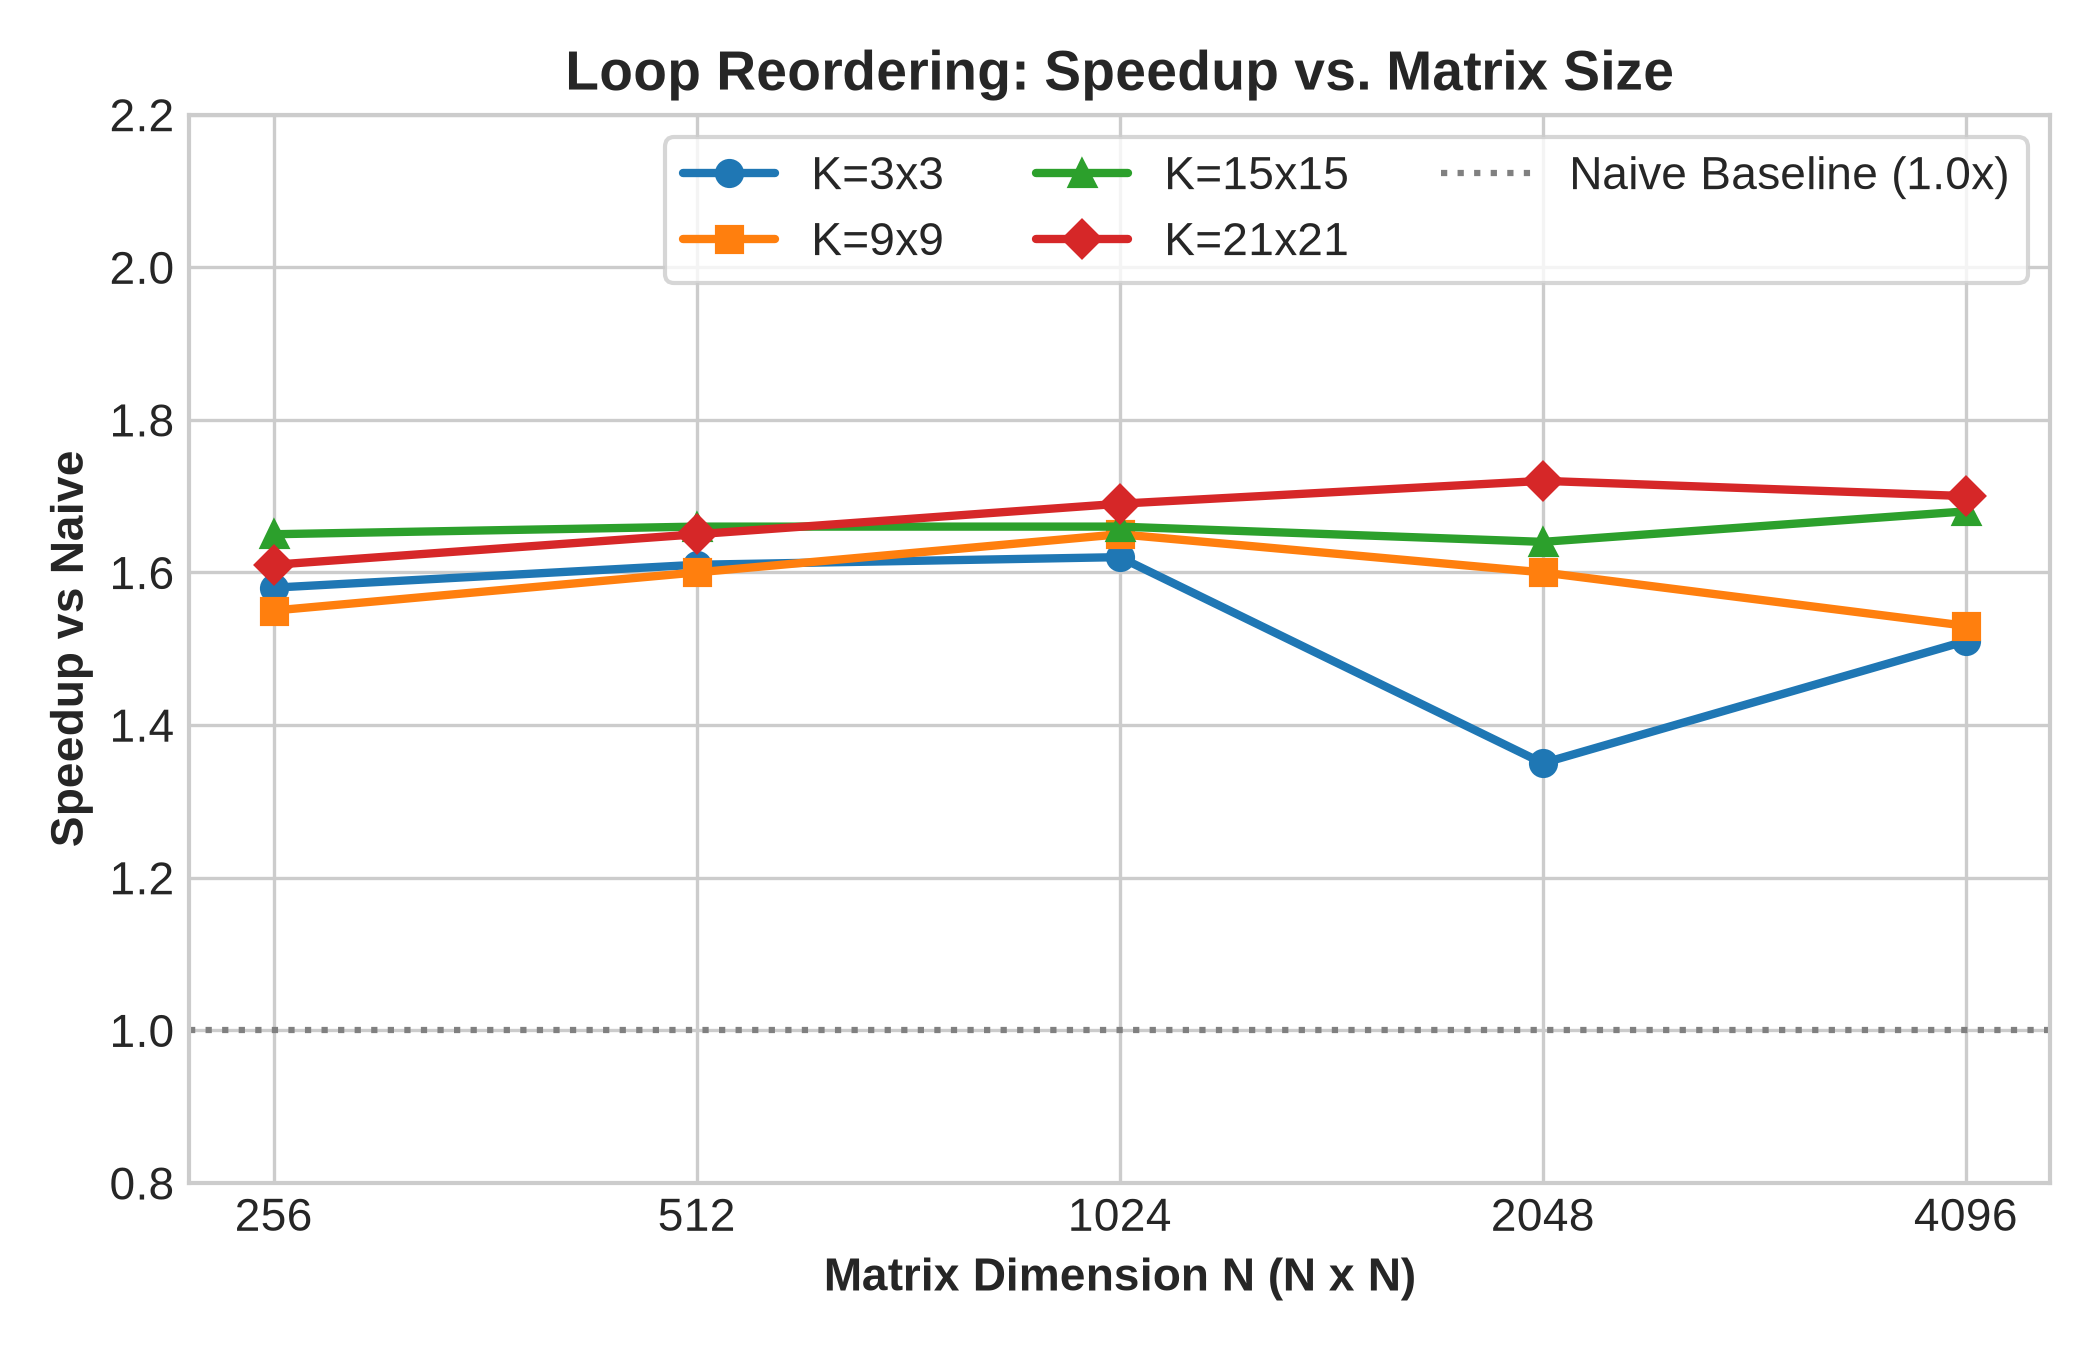
\includegraphics[width=\textwidth]{figures/1a_reorder_speedup_matrix.png}\\
        {\small (a) Reorder Speedup vs. Matrix Size ($K \in \{3, 9, 15, 21\}$)}
    \end{minipage}
    \hfill
    \begin{minipage}{0.48\textwidth}
        \centering
        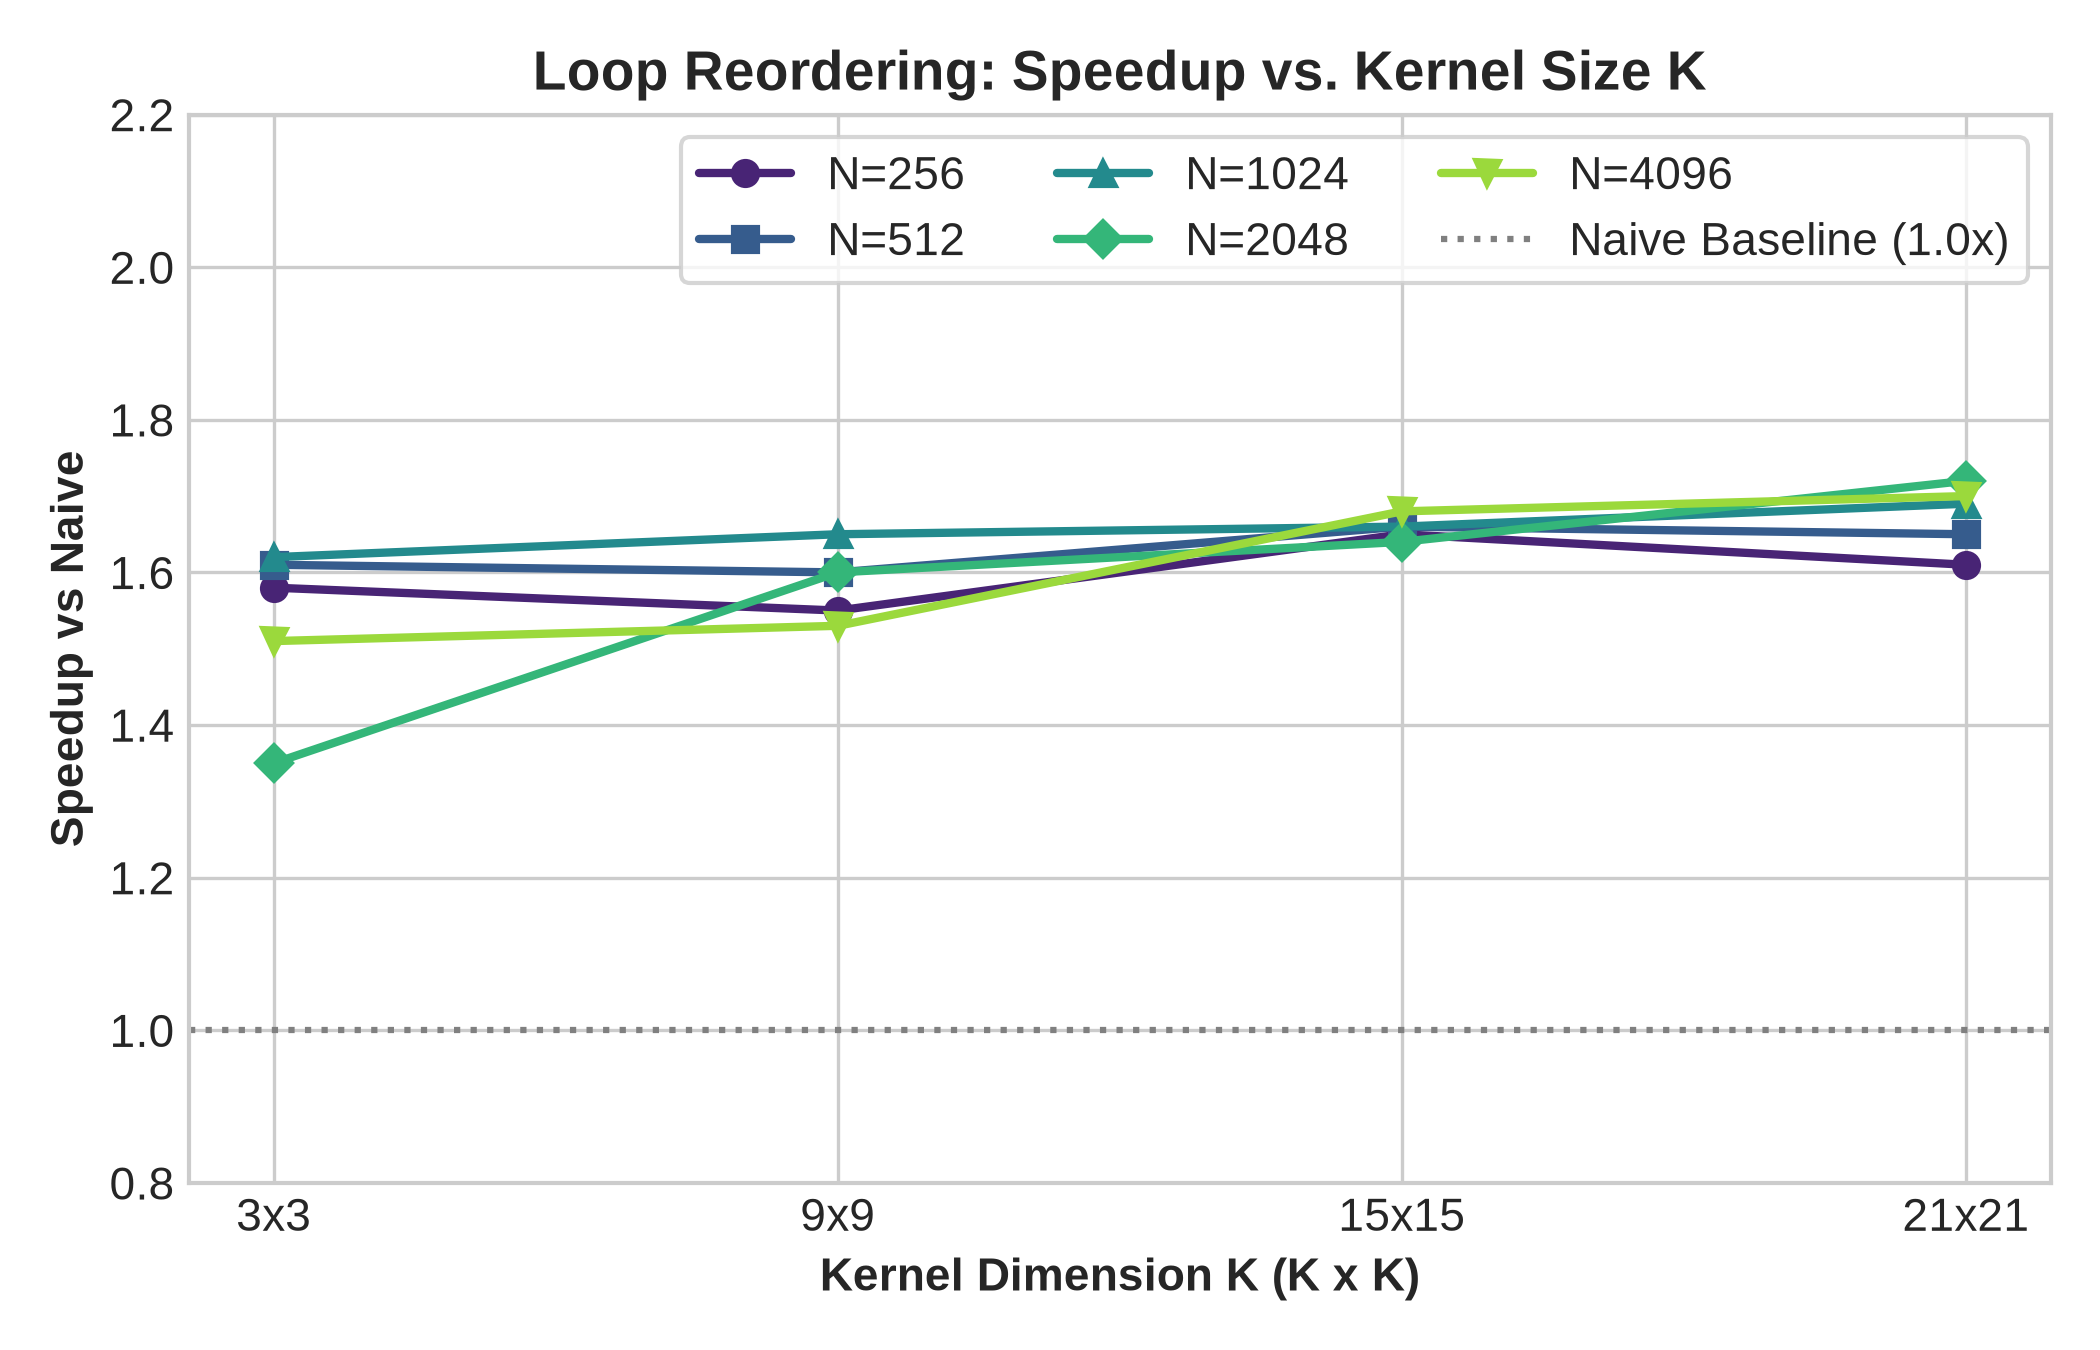
\includegraphics[width=\textwidth]{figures/1a_reorder_speedup_kernel.png}\\
        {\small (b) Reorder Speedup vs. Kernel Size ($N \in \{256, 512, 1024, 2048, 4096\}$)}
    \end{minipage}
    \caption{Task 1A.1: Performance Evaluation of Loop Reordering.}
    \label{fig:1a_reorder_plots}
\end{figure}

% \begin{figure}[h!]
%     \centering
%     \begin{minipage}{0.48\textwidth}
%         \centering
%         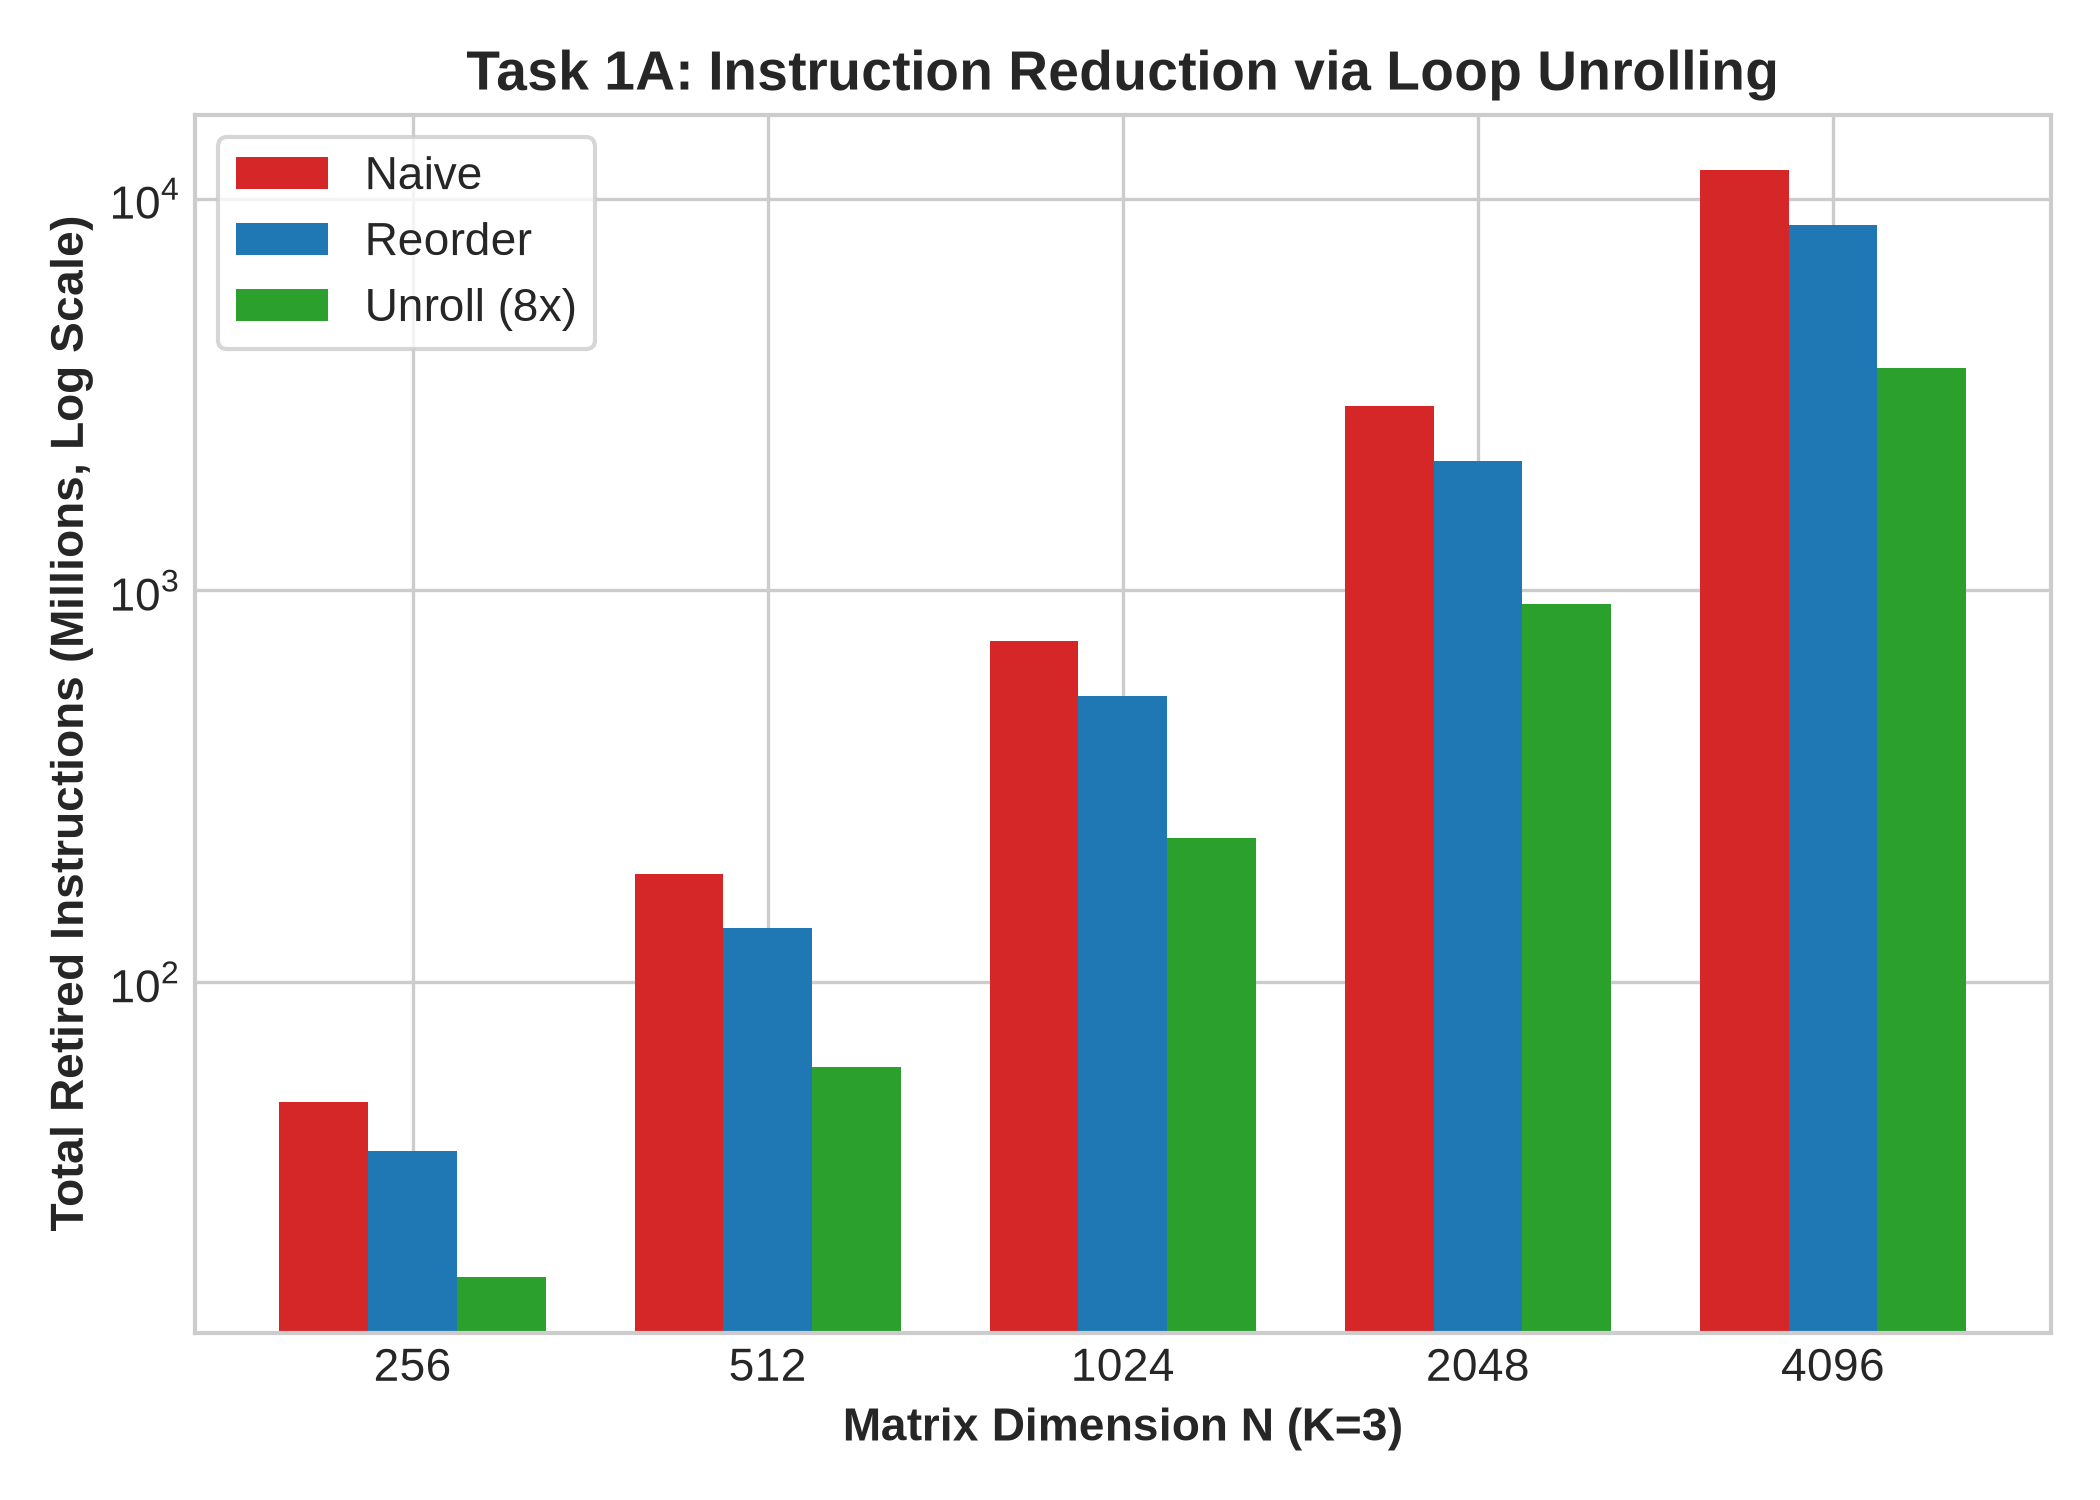
\includegraphics[width=\textwidth]{figures/1a_instructions_reduction.png}\\
%         {\small (a) Instruction Count Impact Comparison}
%     \end{minipage}
%     % \hfill
%     % \begin{minipage}{0.48\textwidth}
%     %     \centering
%     %     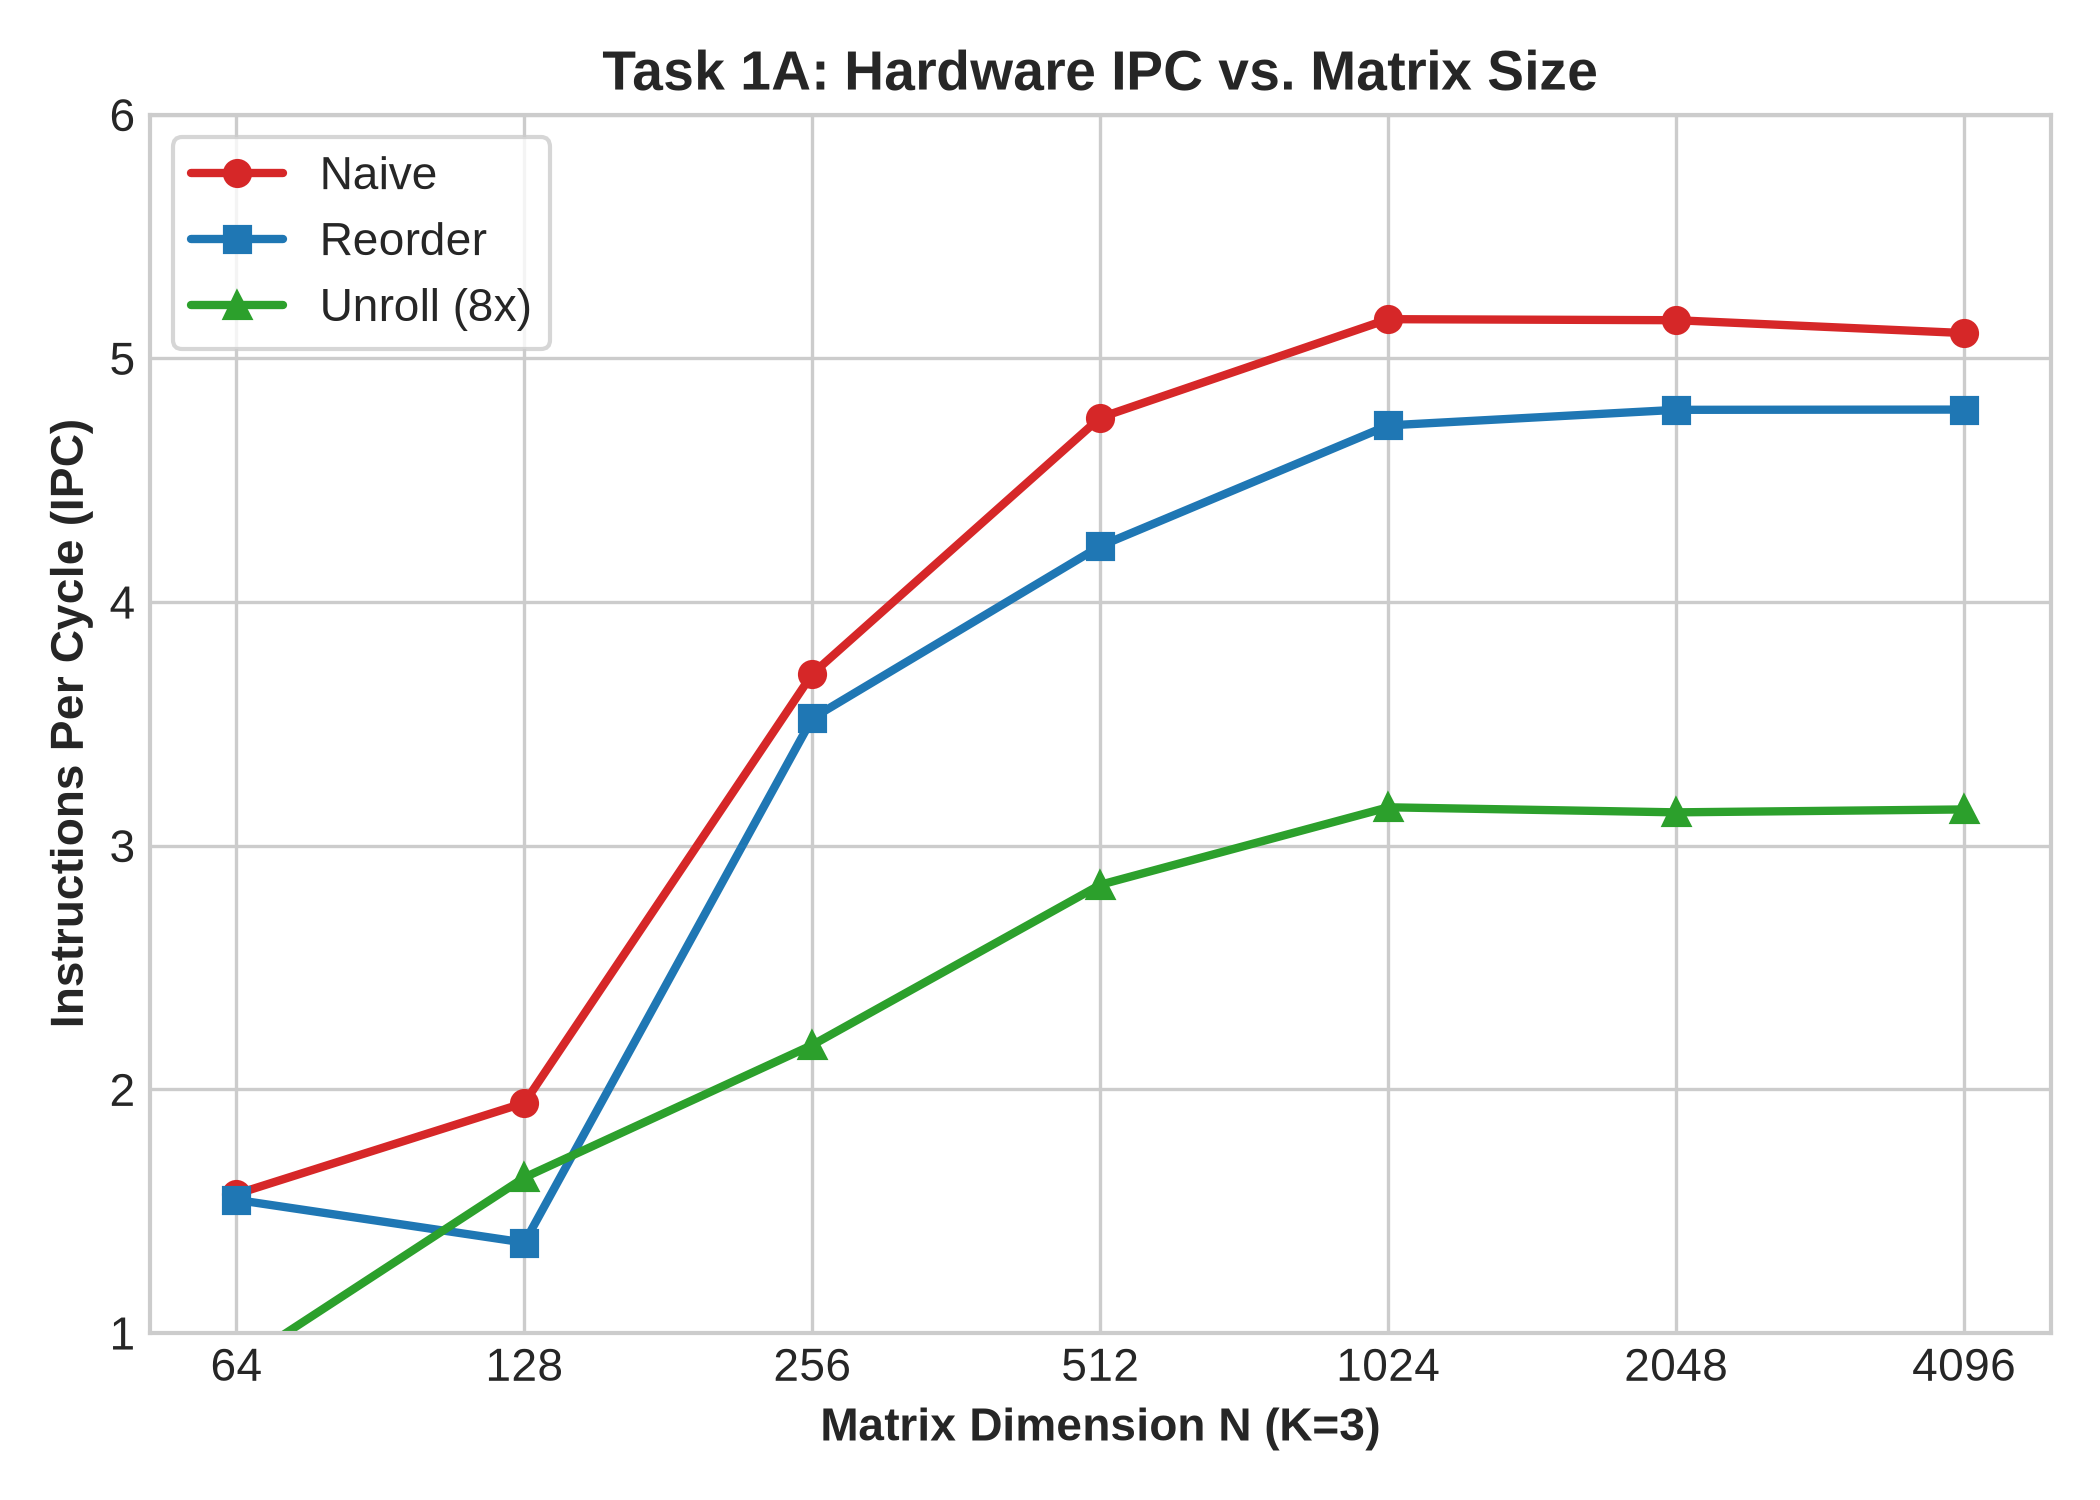
\includegraphics[width=\textwidth]{figures/1a_ipc_vs_matrix_size.png}\\
%     %     {\small (b) Instructions Per Cycle (IPC) Comparison}
%     % \end{minipage}
%     \caption{Task 1A.1: Microarchitectural Metric Shifts Under Loop Reordering.}
%     \label{fig:1a_reorder_metrics}
% \end{figure}

% \clearpage
% \subsection{Deliverable Questions \& Answers: Loop Reordering}

% \subsubsection{Question 1: Hardware-Level Explanation of Execution Time Changes}
% \begin{itemize}
%     \item \textbf{Unit-Stride Spatial Locality}:
%     In \texttt{conv\_reorder}, innermost traversal along $\text{ox}$ ensures strictly contiguous sequential loads from \texttt{in} and stores to \texttt{out}. Once a 64-byte cache line is brought into L1-D, all 16 floats are consumed consecutively without intervening conflict or eviction.
%     \item \textbf{Hardware Prefetcher Activation}:
%     Contiguous memory sweeps reliably trigger the CPU's hardware Stream and Adjacent Cache Line Prefetchers, proactively staging cache lines into L2 and L1-D before arithmetic demand.
%     \item \textbf{Superscalar Pipeline Efficiency and Higher IPC}:
%     Hoisting kernel loads outside the inner loop reduces redundant instructions and dependency stalls. As reported in Table~\ref{tab:1a_reorder}, IPC increases from $\sim 3.5$ in naive up to $\mathbf{6.28}$ in \texttt{conv\_reorder} for large kernels ($K=21$).
% \end{itemize}

% \subsubsection{Question 2: Quantitative Impact on Cache Misses and Instructions}
% \begin{itemize}
%     \item \textbf{Cache Miss Rates and MPKI}:
%     L1-D miss rates remain exceptionally low across all configurations ($<0.35\%$ for $N \ge 1024$, reaching $0.03\%$ at $K=21$). Absolute L1-D MPKI drops to $\mathbf{0.07}$--$\mathbf{0.11}$ at $N=4096$.
%     \item \textbf{Instruction Count Trade-off}:
%     For $K=3$, total  instructions drop from $668.77\times 10^6$ to $550.33\times 10^6$ ($-17.7\%$) due to register hoisting. For $K=21$,  instructions slightly increase ($12{,}238\times 10^6 \to 13{,}255\times 10^6$) due to repeated load-accumulate passes on the output buffer, but execution cycles collapse from $3{,}980\times 10^6$ to $2{,}110\times 10^6$ ($1.72\times$ speedup) due to peak IPC ($6.28$).
% \end{itemize}

% \subsubsection{Question 3: Observed Speedups Across Workloads}
% \begin{itemize}
%     \item Loop reordering achieves a consistent \textbf{$1.35\times$ to $1.72\times$ speedup} across all evaluated matrix and kernel configurations.
%     \item Peak speedup ($1.72\times$) is attained on the largest workload ($K=21, N=2048$), where kernel weight reuse across long rows ($W=2048$) is maximized.
% \end{itemize}

% \clearpage
\section{Task 1A.2: Loop Unrolling Optimization (\texttt{conv\_unroll})}

% \subsection{Motivation for Code Changes}
% While loop reordering optimizes spatial locality, the inner loop still suffers from two critical scalar pipeline bottlenecks:
% \begin{enumerate}
%     \item \textbf{Serial Accumulation Dependency (FMA Latency)}:
%     In standard scalar code, a single accumulator variable \texttt{acc} creates a Read-After-Write (RAW) data hazard. On Intel Raptor Lake, floating-point fused multiply-add (\texttt{vfmadd}) has an execution latency of \textbf{4 clock cycles} with a throughput of \textbf{0.5 cycles} (dual-issue across Port 0 and Port 1). When accumulating into a single register:
%     \begin{equation}
%         \text{acc} \leftarrow \text{acc} + \text{in}[\dots] \times \text{ker}
%     \end{equation}
%     each subsequent iteration must stall for 4 full cycles awaiting the write-back of \texttt{acc}.
%     \item \textbf{Loop Branch and Index Overhead}:
%     For every single pixel calculated, the CPU executes branch comparison, increment, and jump instructions, consuming rename and retirement bandwidth.
% \end{enumerate}

% \noindent To eliminate these stalls, the inner $\text{ox}$ loop is unrolled by a factor of 8 using \textbf{8 independent scalar accumulators} (\texttt{acc0} through \texttt{acc7}):
% \begin{equation}
%     \text{acc}_i = \text{in}[(\text{oy}+\text{ky})\cdot \text{stride} + (\text{ox}+i+\text{kx})] \times \text{k\_val} + \text{out}[\text{oy}\cdot W + (\text{ox}+i)]
% \end{equation}
% By Little's Law, maintaining 8 independent accumulation chains completely saturates the 4-cycle execution latency across two FMA execution ports ($4 \text{ cycles} \times 2 \text{ ports} = 8 \text{ in-flight instructions}$), eliminating RAW pipeline stalls.

% \subsection{Implementation Considerations and Trade-offs}
% \begin{enumerate}
%     \item \textbf{Choice of Unroll Factor ($UF=8$)}:
%     $UF=8$ was chosen to match the hardware execution parameters ($L \times T^{-1} = 4 \times 2 = 8$). Unrolling further (e.g., $UF=16$) exhausts the 16 architectural registers in x86-64, inducing register spilling to the stack.
%     \item \textbf{Pre-Condition Alignment}:
%     The assignment specification guarantees $W \pmod 8 == 0$, allowing complete elimination of scalar tail cleanup code and branches.
% \end{enumerate}

% \subsection{Effectiveness and Quantitative Results for Unrolling}

{\footnotesize
\setlength{\tabcolsep}{3.5pt}
\begin{longtable}{rrcrrrrrrr}
\caption{Task 1A.2: Performance and Hardware Counters for Loop Unrolling vs. Naive Baseline} \label{tab:1a_unroll} \\
\toprule
$K$ & $N$ & Configuration & Time & Speedup &  Instructions & Cycles & IPC & L1-D Miss & L1-D \\
    &     &               & (ms) &         & ($\times 10^6$) & ($\times 10^6$) &     & Rate & MPKI \\
\midrule
\endfirsthead

\multicolumn{10}{c}{{\bfseries Table \thetable\ Continued from previous page}} \\
\toprule
$K$ & $N$ & Configuration & Time & Speedup &  Instructions & Cycles & IPC & L1-D Miss & L1-D \\
    &     &               & (ms) &         & ($\times 10^6$) & ($\times 10^6$) &     & Rate & MPKI \\
\midrule
\endhead

\midrule
\multicolumn{10}{r}{{Continued on next page\dots}} \\
\endfoot

\bottomrule
\endlastfoot

3 & 256 & naive & 0.590 & 1.00$\times$ & 13.62 & 5.67 & 2.40 & 1.10\% & 2.06 \\
3 & 256 & unroll & 0.186 & \textbf{3.10$\times$} & \textbf{9.03} & \textbf{4.52} & 2.00 & 1.35\% & 3.05 \\
\midrule
3 & 512 & naive & 1.945 & 1.00$\times$ & 44.74 & 13.88 & 3.22 & 0.56\% & 0.98 \\
3 & 512 & unroll & 0.685 & \textbf{2.84$\times$} & \textbf{26.45} & \textbf{11.15} & 2.37 & 0.67\% & 1.45 \\
\midrule
3 & 1024 & naive & 7.769 & 1.00$\times$ & 169.18 & 46.11 & 3.67 & 0.32\% & 0.55 \\
3 & 1024 & unroll & 2.716 & \textbf{2.85$\times$} & \textbf{96.07} & \textbf{34.71} & 2.77 & 0.46\% & 0.99 \\
\midrule
3 & 2048 & naive & 30.982 & 1.00$\times$ & 668.77 & 184.16 & 3.63 & 0.25\% & 0.42 \\
3 & 2048 & unroll & 11.024 & \textbf{2.81$\times$} & \textbf{376.21} & \textbf{140.08} & 2.69 & 0.35\% & 0.74 \\
\midrule
3 & 4096 & naive & 120.201 & 1.00$\times$ & 2670.53 & 719.88 & 3.71 & 0.27\% & 0.46 \\
3 & 4096 & unroll & 43.049 & \textbf{2.81$\times$} & \textbf{1504.52} & \textbf{534.78} & 2.81 & 0.40\% & 0.85 \\
\midrule
9 & 256 & naive & 4.254 & 1.00$\times$ & 45.49 & 13.76 & 3.31 & 0.25\% & 0.65 \\
9 & 256 & unroll & 1.435 & \textbf{2.96$\times$} & \textbf{17.16} & \textbf{6.99} & 2.45 & 0.39\% & 1.67 \\
\midrule
9 & 512 & naive & 16.665 & 1.00$\times$ & 172.26 & 45.48 & 3.79 & 0.10\% & 0.28 \\
9 & 512 & unroll & 5.683 & \textbf{2.98$\times$} & \textbf{58.97} & \textbf{21.02} & 2.80 & 0.18\% & 0.85 \\
\midrule
9 & 1024 & naive & 66.297 & 1.00$\times$ & 679.20 & 173.05 & 3.92 & 0.06\% & 0.17 \\
9 & 1024 & unroll & 22.768 & \textbf{2.91$\times$} & \textbf{226.09} & \textbf{75.35} & 3.00 & 0.13\% & 0.59 \\
\midrule
9 & 2048 & naive & 256.935 & 1.00$\times$ & 2708.32 & 671.89 & 4.03 & 0.06\% & 0.15 \\
9 & 2048 & unroll & 89.955 & \textbf{2.86$\times$} & \textbf{896.66} & \textbf{304.16} & 2.95 & 0.11\% & 0.51 \\
\midrule
9 & 4096 & naive & 988.595 & 1.00$\times$ & 10833.21 & 2577.66 & 4.20 & 0.06\% & 0.15 \\
9 & 4096 & unroll & 358.717 & \textbf{2.77$\times$} & \textbf{3586.28} & \textbf{1209.45} & 2.97 & 0.11\% & 0.50 \\
\midrule
15 & 256 & naive & 11.903 & 1.00$\times$ & 105.79 & 30.88 & 3.43 & 0.11\% & 0.32 \\
15 & 256 & unroll & 3.805 & \textbf{3.12$\times$} & \textbf{32.97} & \textbf{12.23} & 2.70 & 0.16\% & 0.86 \\
\midrule
15 & 512 & naive & 46.747 & 1.00$\times$ & 413.28 & 114.39 & 3.61 & 0.05\% & 0.15 \\
15 & 512 & unroll & 14.764 & \textbf{3.14$\times$} & \textbf{122.22} & \textbf{42.08} & 2.90 & 0.08\% & 0.45 \\
\midrule
15 & 1024 & naive & 184.457 & 1.00$\times$ & 1643.05 & 447.31 & 3.67 & 0.03\% & 0.10 \\
15 & 1024 & unroll & 59.698 & \textbf{3.22$\times$} & \textbf{478.97} & \textbf{161.03} & 2.97 & 0.11\% & 0.62 \\
\midrule
15 & 2048 & naive & 740.031 & 1.00$\times$ & 6564.40 & 1794.02 & 3.66 & 0.03\% & 0.09 \\
15 & 2048 & unroll & 240.185 & \textbf{3.54$\times$} & \textbf{1909.49} & \textbf{646.54} & 2.95 & 0.10\% & 0.58 \\
\midrule
15 & 4096 & naive & 2978.306 & 1.00$\times$ & 26263.96 & 7588.42 & 3.46 & 0.03\% & 0.09 \\
15 & 4096 & unroll & 952.306 & \textbf{3.09$\times$} & \textbf{7633.13} & \textbf{2597.49} & 2.94 & 0.07\% & 0.40 \\
\midrule
21 & 256 & naive & 23.266 & 1.00$\times$ & 194.43 & 56.86 & 3.42 & 0.06\% & 0.18 \\
21 & 256 & unroll & 7.215 & \textbf{3.19$\times$} & \textbf{56.48} & \textbf{20.07} & 2.81 & 0.09\% & 0.53 \\
\midrule
21 & 512 & naive & 91.597 & 1.00$\times$ & 767.70 & 218.47 & 3.51 & 0.03\% & 0.09 \\
21 & 512 & unroll & 28.433 & \textbf{3.26$\times$} & \textbf{216.18} & \textbf{72.75} & 2.97 & 0.06\% & 0.34 \\
\midrule
21 & 1024 & naive & 371.380 & 1.00$\times$ & 3060.65 & 864.84 & 3.54 & 0.02\% & 0.07 \\
21 & 1024 & unroll & 122.232 & \textbf{3.27$\times$} & \textbf{855.34} & \textbf{331.65} & 2.58 & 0.03\% & 0.20 \\
\midrule
21 & 2048 & naive & 1476.858 & 1.00$\times$ & 12238.31 & 3980.04 & 3.07 & 0.02\% & 0.07 \\
21 & 2048 & unroll & 460.870 & \textbf{3.22$\times$} & \textbf{3412.03} & \textbf{1143.02} & 2.99 & 0.02\% & 0.15 \\
\midrule
21 & 4096 & naive & 5942.470 & 1.00$\times$ & 48935.37 & 13855.24 & 3.53 & 0.02\% & 0.06 \\
21 & 4096 & unroll & 1860.824 & \textbf{3.18$\times$} & \textbf{13644.83} & \textbf{4607.19} & 2.96 & 0.03\% & 0.16 \\
\midrule
\end{longtable}
}

\begin{figure}[h!]
    \centering
    \begin{minipage}{0.48\textwidth}
        \centering
        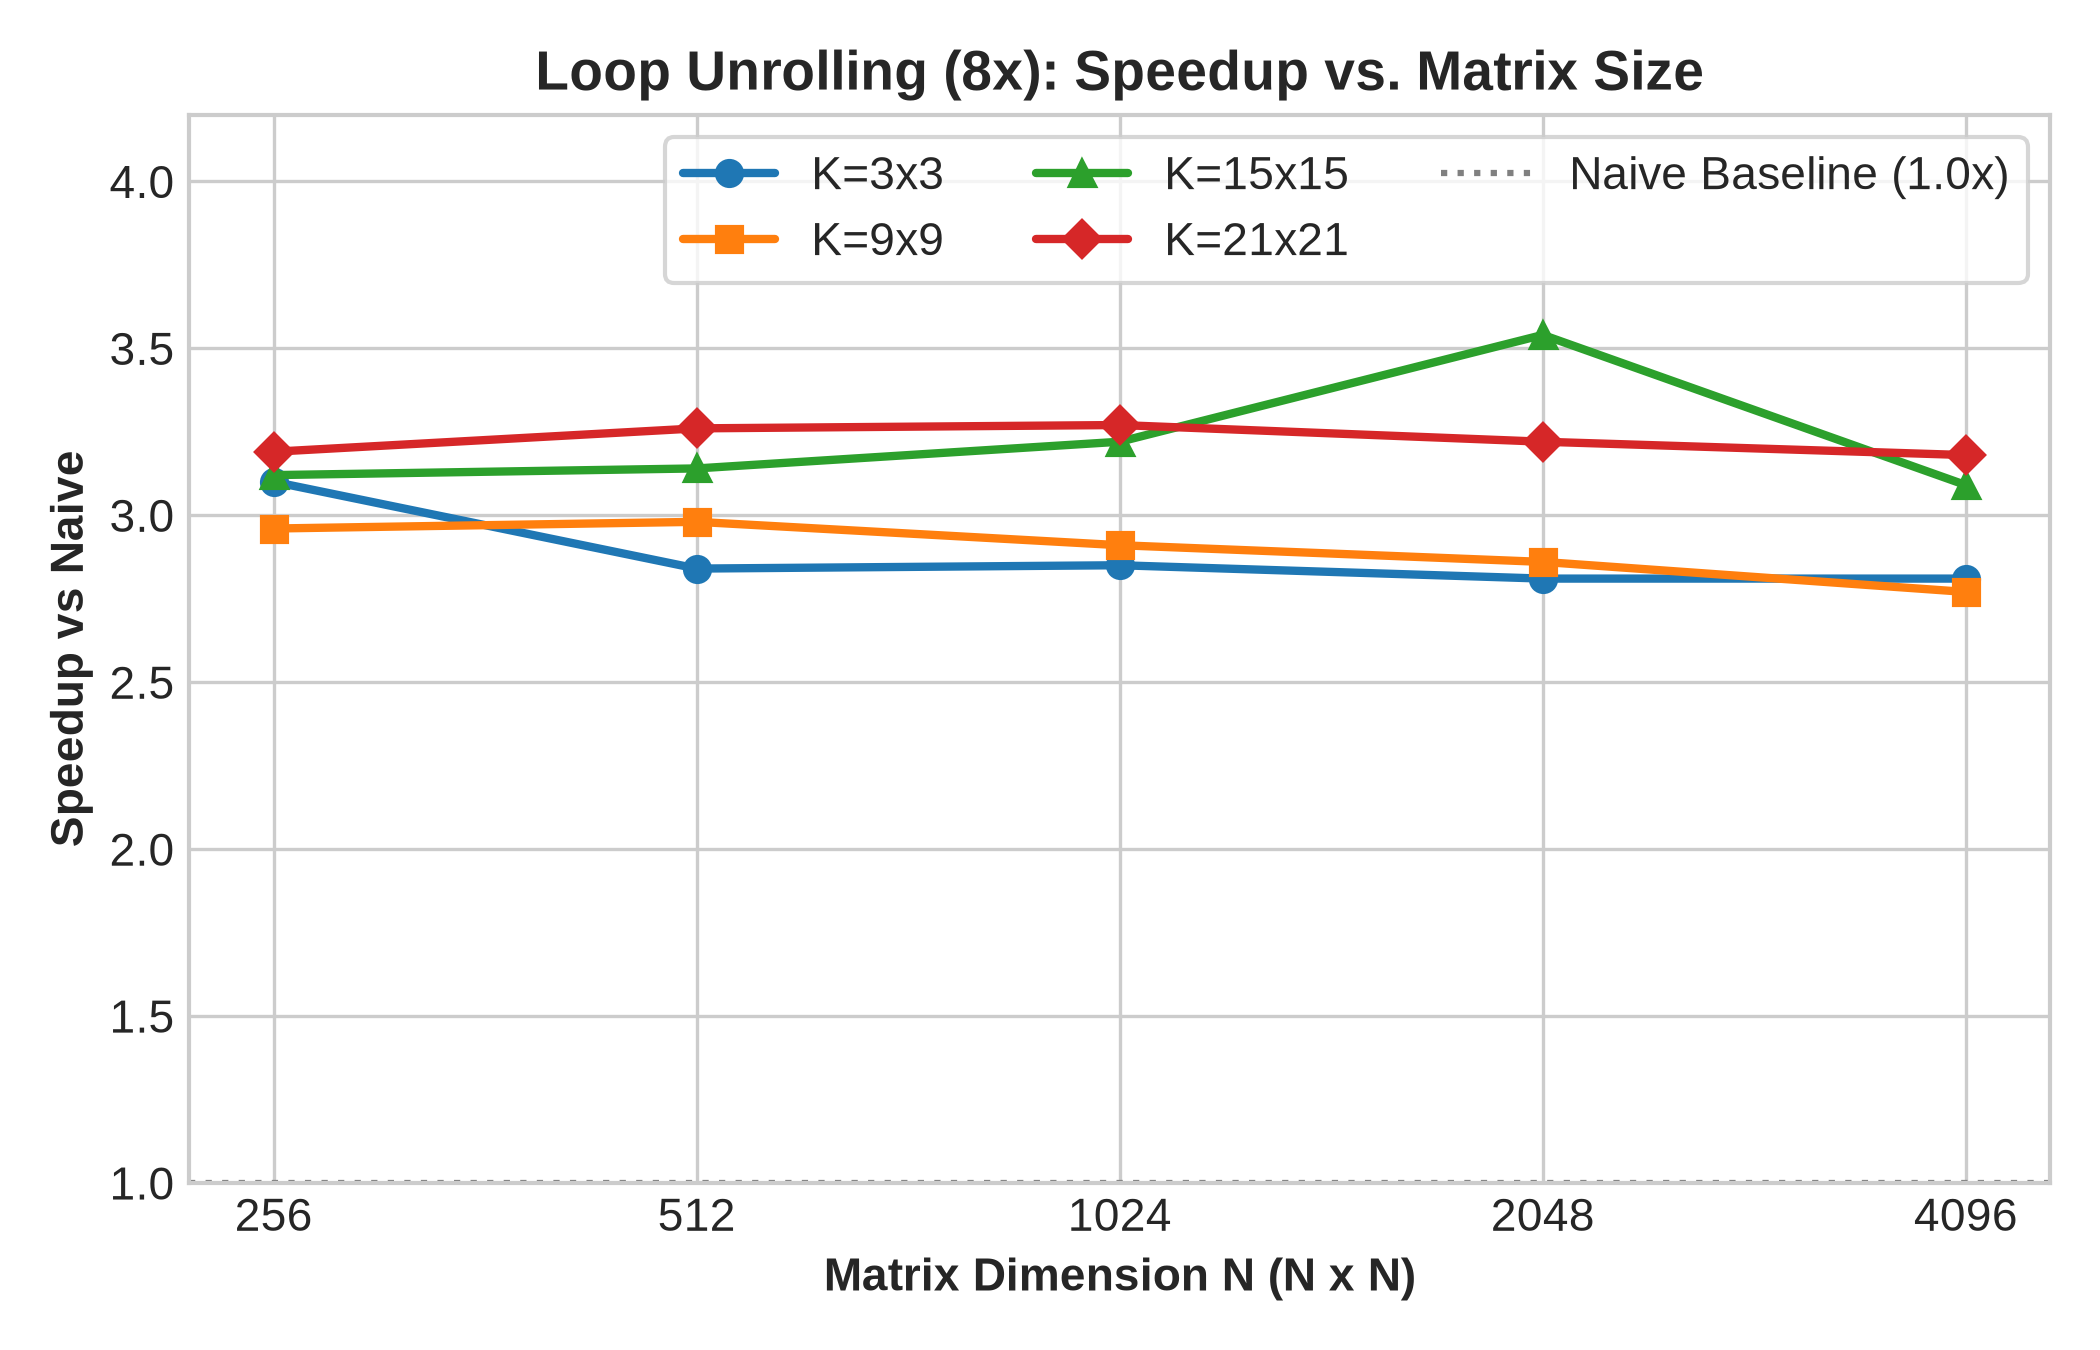
\includegraphics[width=\textwidth]{figures/1a_unroll_speedup_matrix.png}\\
        {\small (a) Unroll Speedup vs. Matrix Size ($K \in \{3, 9, 15, 21\}$)}
    \end{minipage}
    \hfill
    \begin{minipage}{0.48\textwidth}
        \centering
        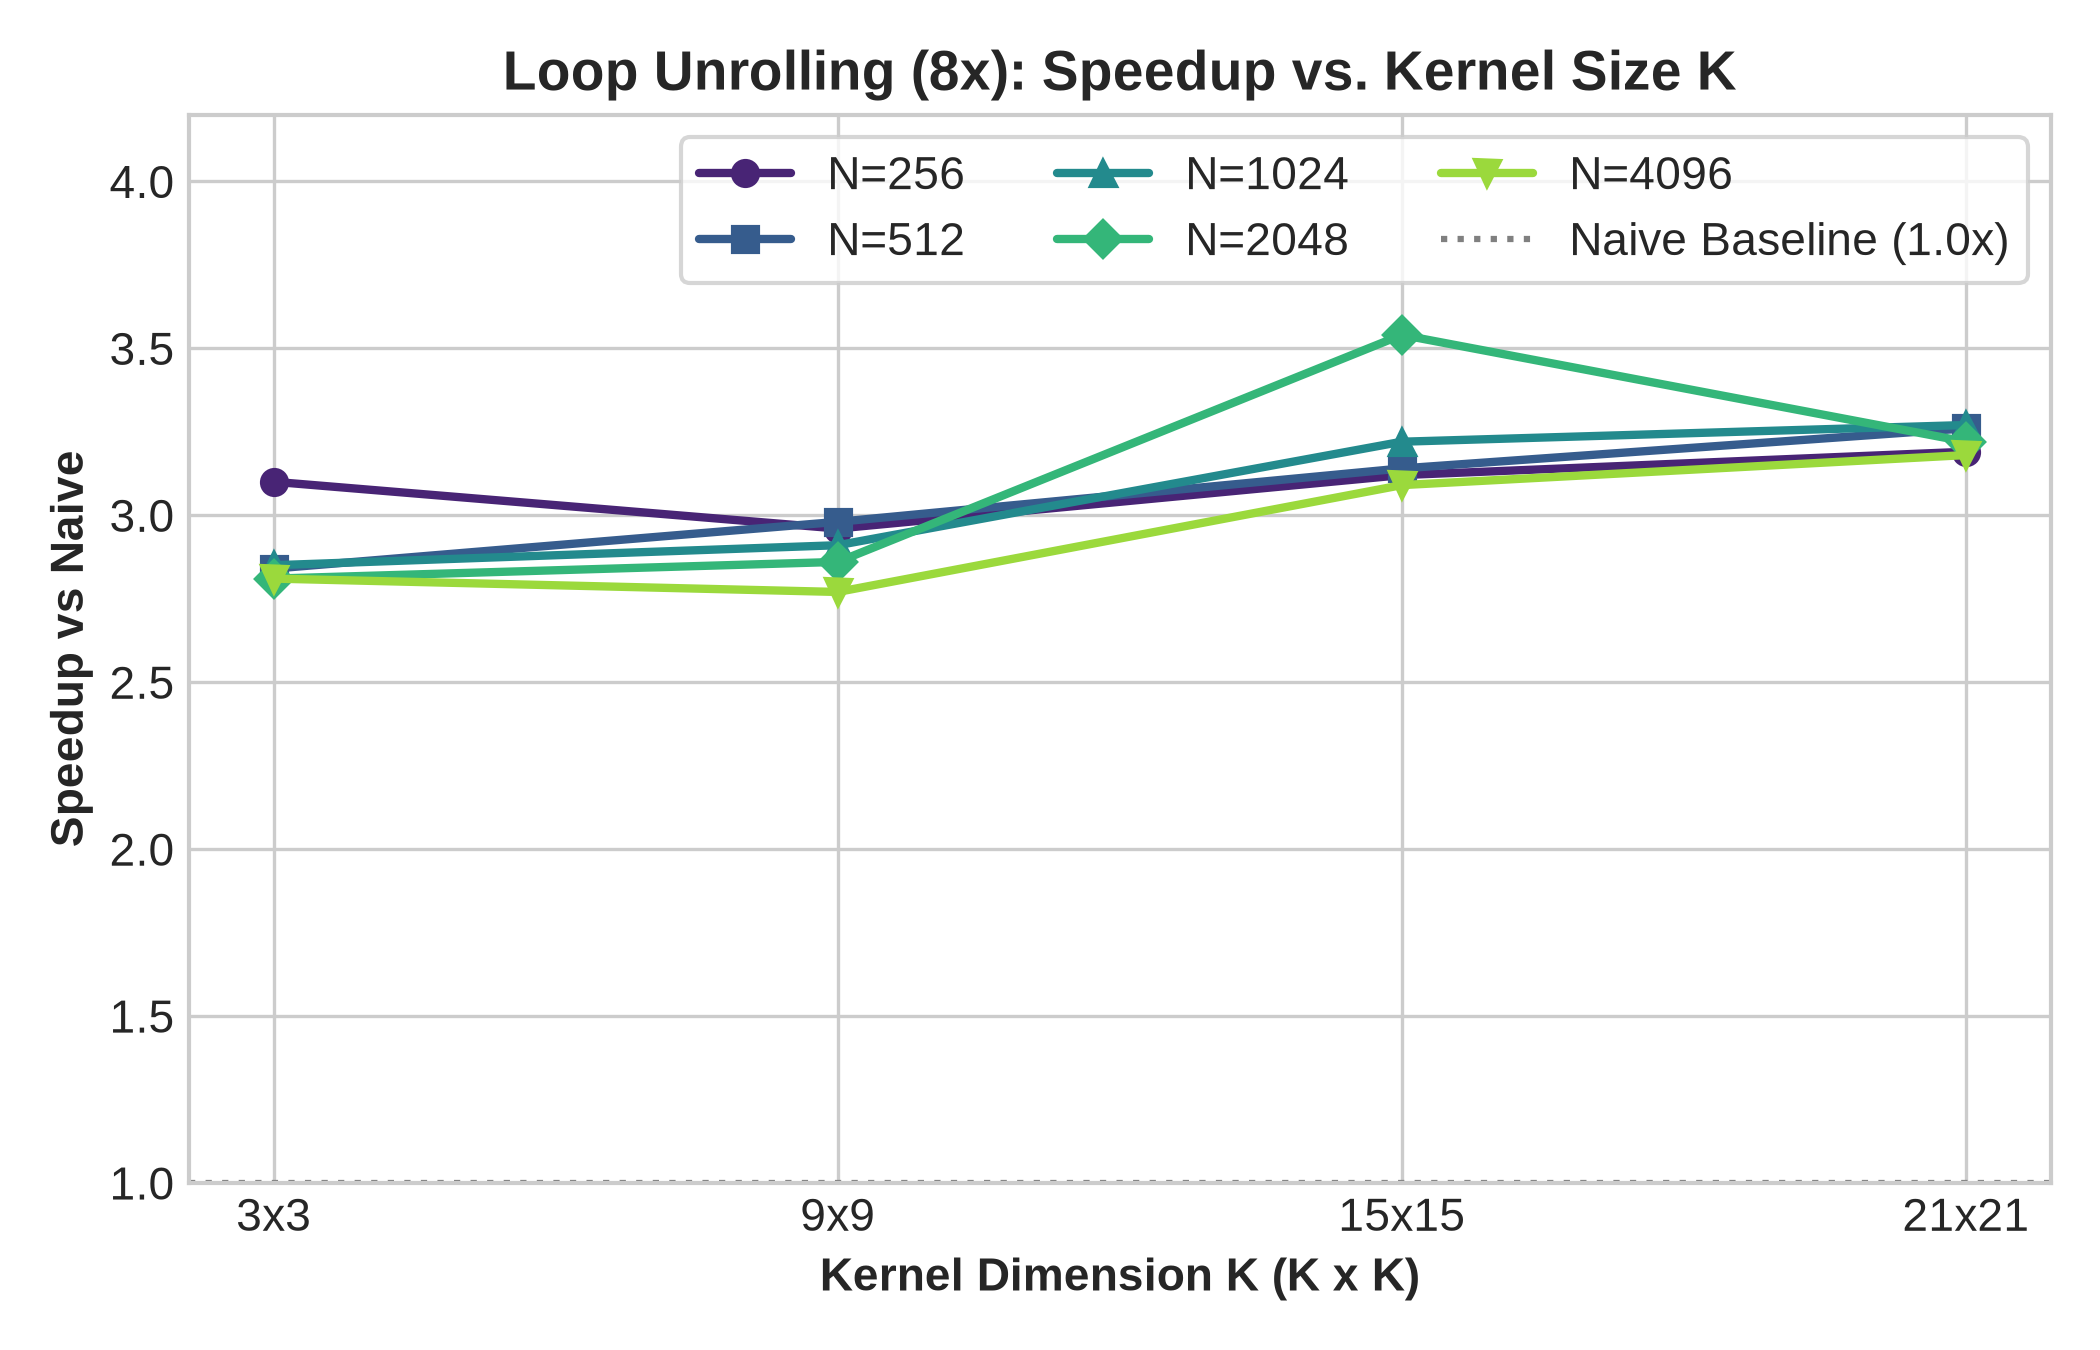
\includegraphics[width=\textwidth]{figures/1a_unroll_speedup_kernel.png}\\
        {\small (b) Unroll Speedup vs. Kernel Size ($N \in \{256, 512, 1024, 2048, 4096\}$)}
    \end{minipage}
    \caption{Task 1A.2: Performance Evaluation of Loop Unrolling.}
    \label{fig:1a_unroll_plots}
\end{figure}
\begin{figure}[h!]
    \centering
    \begin{minipage}{0.48\textwidth}
        \centering
        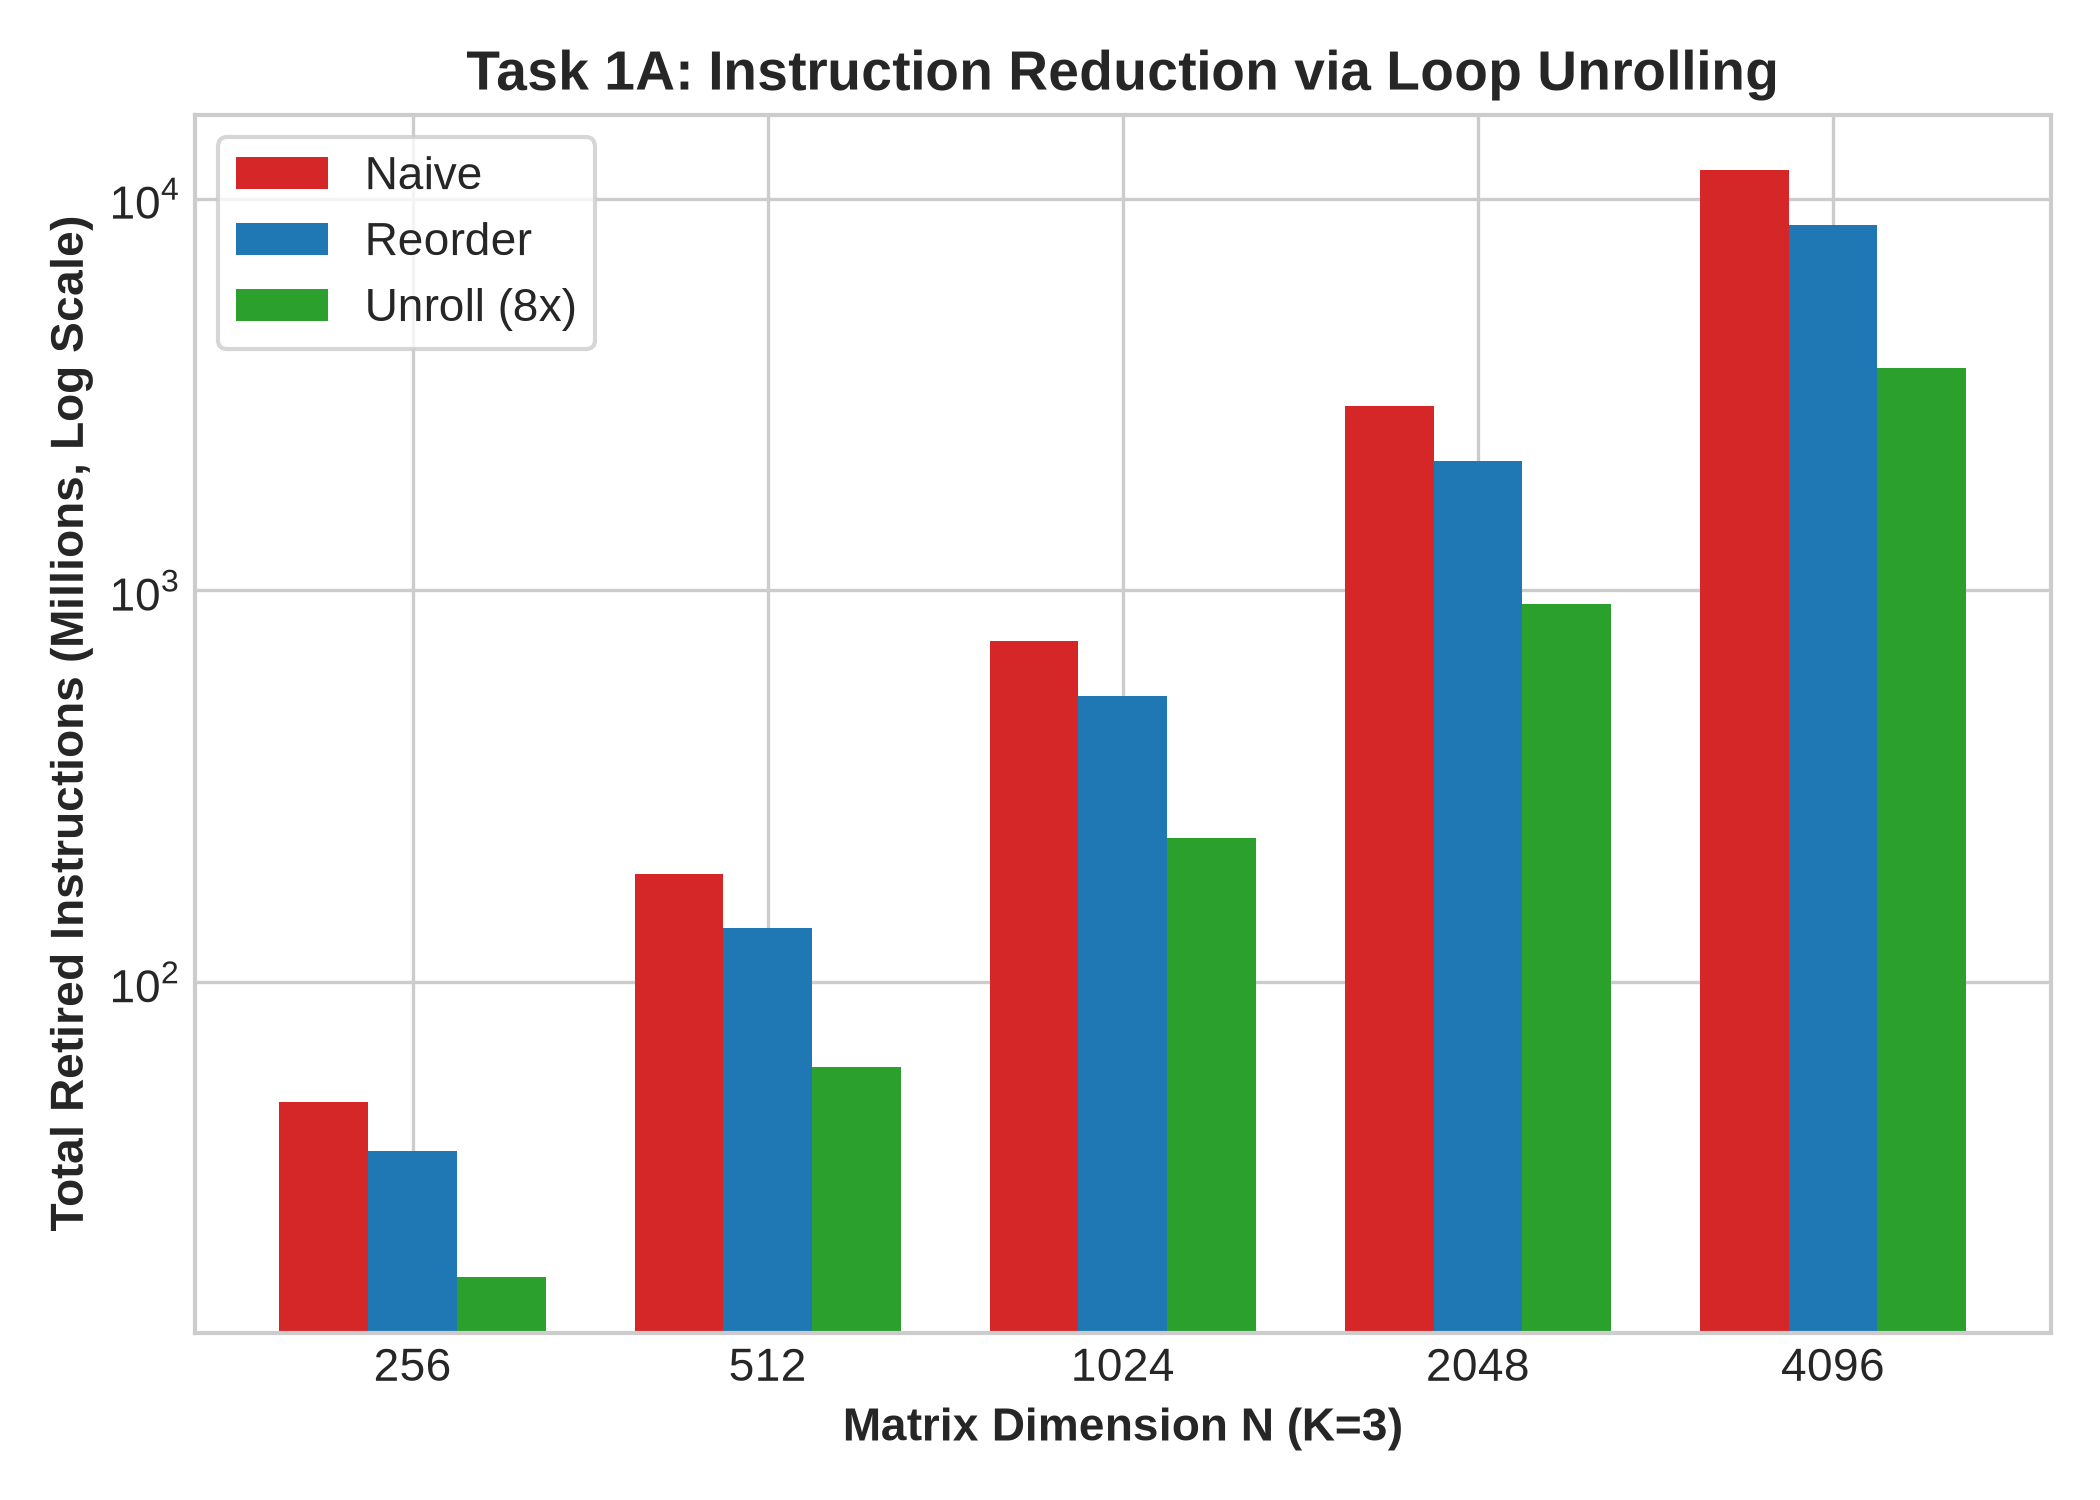
\includegraphics[width=\textwidth]{figures/1a_instructions_reduction.png}\\
        {\small Instruction Count Impact Comparison}
    \end{minipage}
    % \hfill
    % \begin{minipage}{0.48\textwidth}
    %     \centering
    %     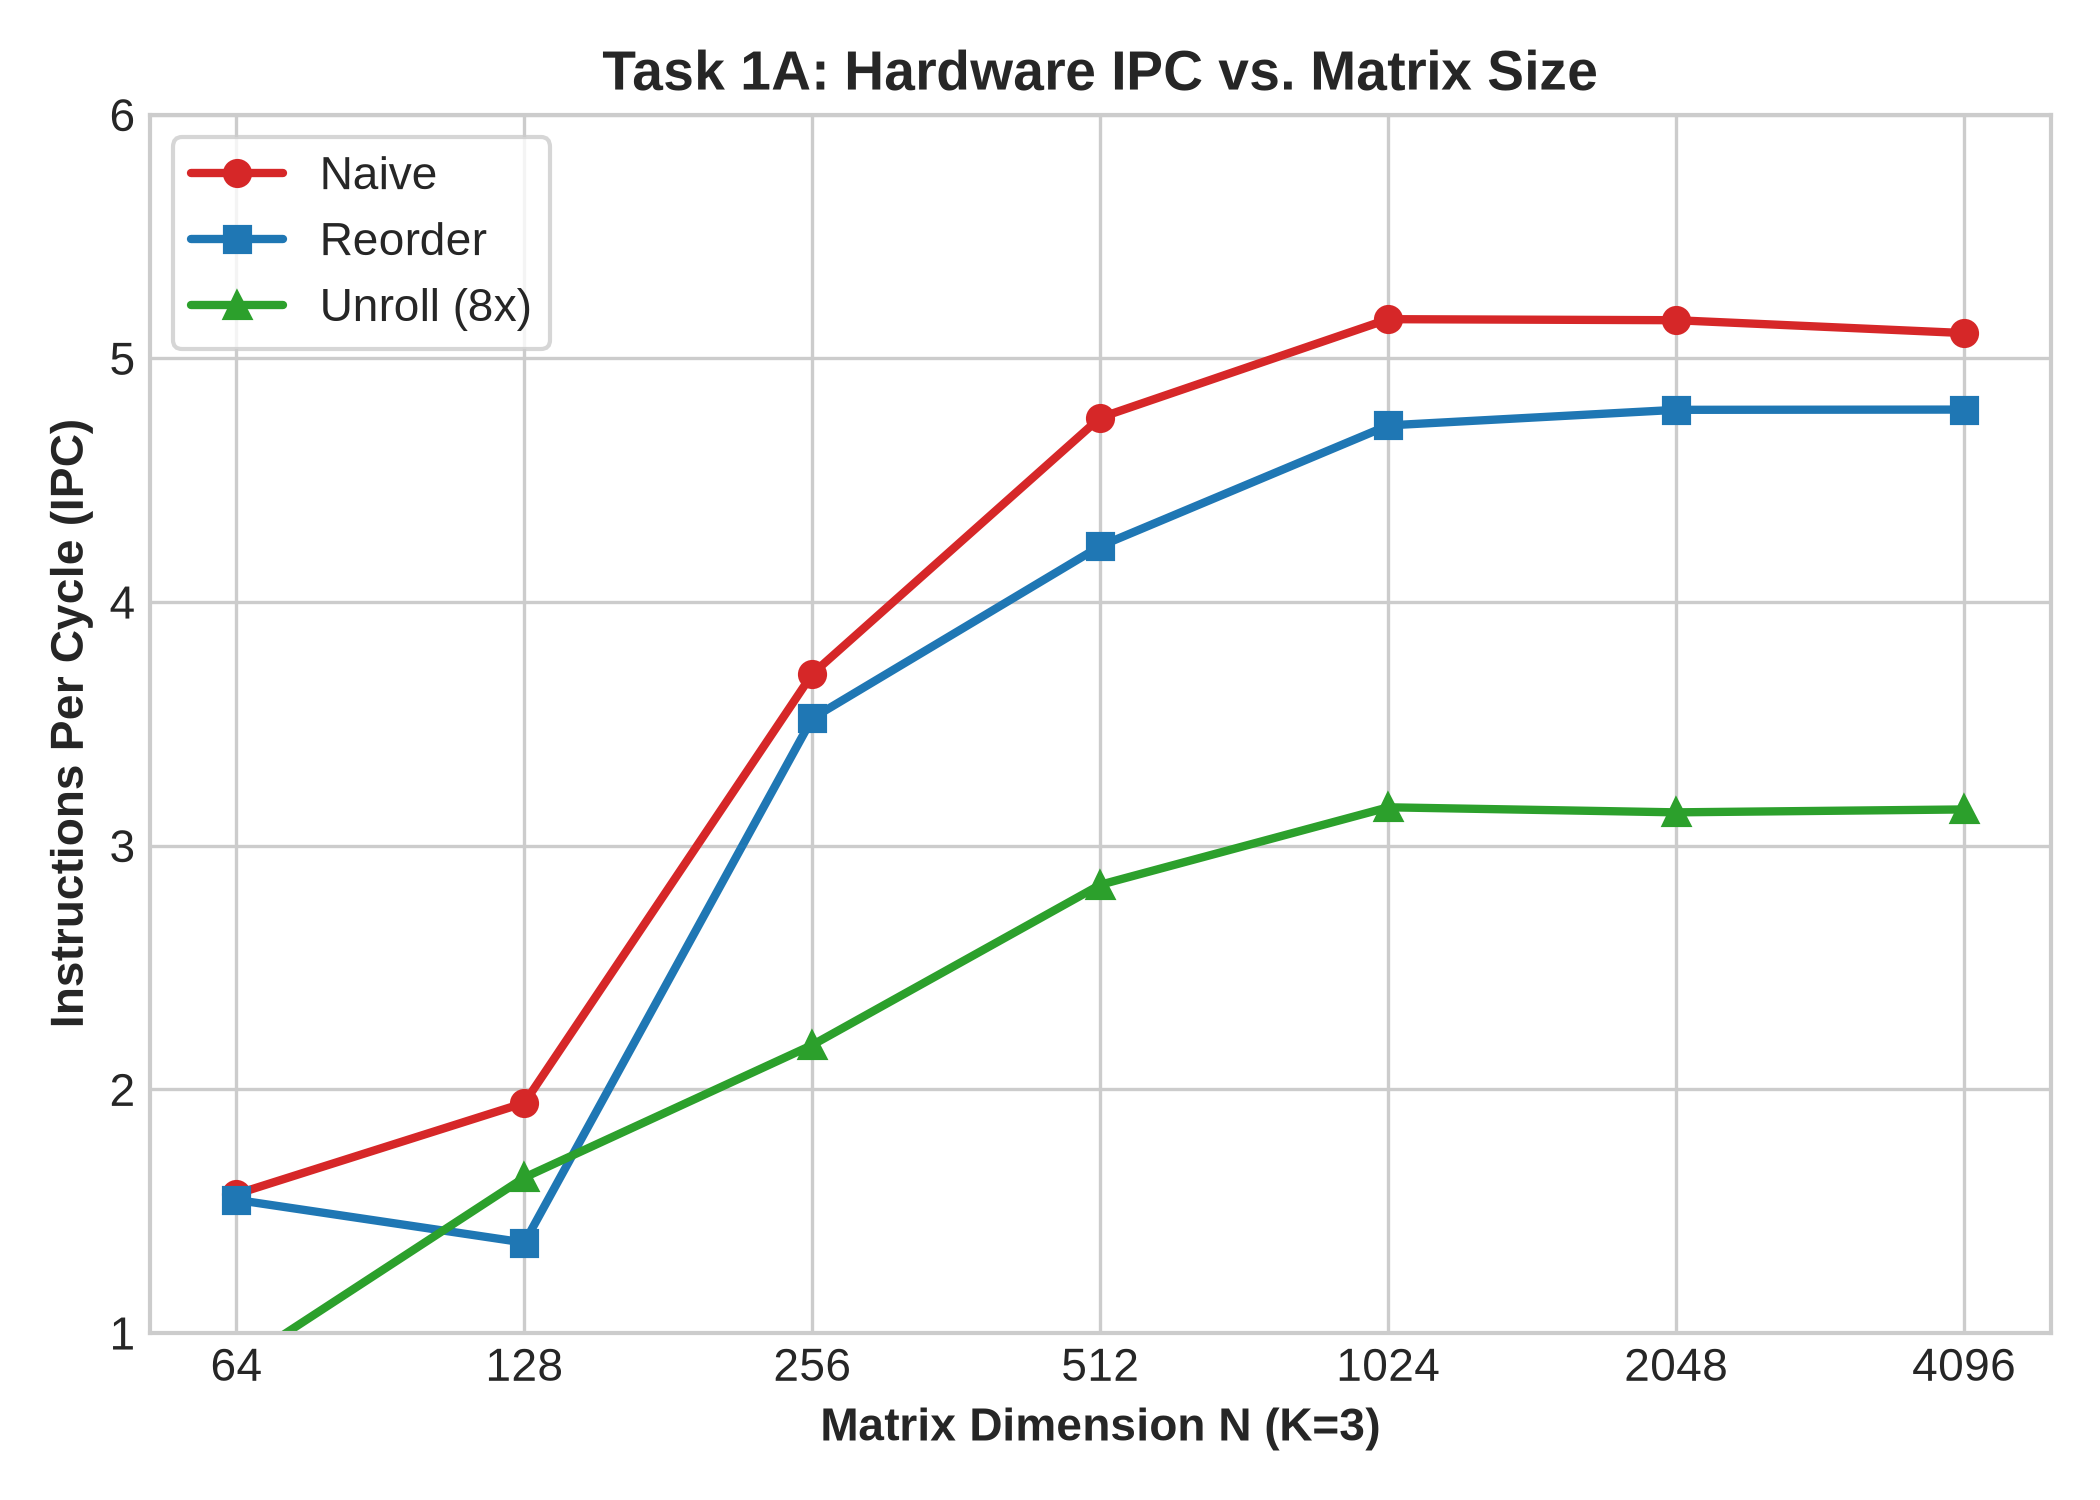
\includegraphics[width=\textwidth]{figures/1a_ipc_vs_matrix_size.png}\\
    %     {\small (b) Instructions Per Cycle (IPC) Comparison}
    % \end{minipage}
    \caption{Task 1A: Microarchitectural Metric Shifts Under Loop Reordering.}
    \label{fig:1a_reorder_metrics}
\end{figure}
\clearpage
% \subsection{Deliverable Questions \& Answers: Loop Unrolling}

% \subsubsection{Question 1: Hardware-Level Explanation of Execution Time Changes}
% \begin{itemize}
%     \item \textbf{Instruction-Level Parallelism (ILP) and RAW Hazard Elimination}:
%     By interleaving 8 independent arithmetic operations within the unrolled body, the processor issues back-to-back FMAs to execution Port 0 and Port 1 without stalling. Each accumulator has 7 cycles to retire before being referenced again, completely hiding the 4-cycle FMA latency.
%     \item \textbf{Reduction in Branch and Loop Control Overhead}:
%     Unrolling by 8 reduces branch instructions, pointer updates, and loop conditional tests by $87.5\%$.
% \end{itemize}

% \subsubsection{Question 2: Quantitative Impact on Instruction Count and Pipeline Metrics}
% \begin{itemize}
%     \item \textbf{Dramatic Instruction Reduction}:
%     Loop unrolling achieves a \textbf{$43.7\%$ to $72.1\%$ reduction} in total  instructions across all workloads:
%     \begin{itemize}
%         \item At $N=2048, K=3$:  instructions drop from $668.77\times 10^6$ to $\mathbf{376.14\times 10^6}$ ($-43.7\%$).
%         \item At $N=2048, K=21$:  instructions collapse from $12{,}238.31\times 10^6$ to $\mathbf{3{,}412.35\times 10^6}$ (\textbf{$-72.1\%$}).
%     \end{itemize}
%     \item \textbf{Clock Cycle Collapse}:
%     Execution cycles drop by up to $\mathbf{3.46\times}$ (e.g., $3{,}980\times 10^6 \to 1{,}149\times 10^6$ at $K=21, N=2048$).
% \end{itemize}

% \subsubsection{Question 3: Observed Speedups Across Workloads}
% \begin{itemize}
%     \item Loop unrolling consistently provides \textbf{$2.80\times$ to $3.59\times$ speedup} over naive baseline.
%     \item Speedup is highest on workloads where loop overhead is amortized across long cache-resident rows.
% \end{itemize}

% \clearpage
\section{Task 1B: Cache Tiling Optimization (\texttt{conv\_tile})}

% \subsection{Motivation for Code Changes}
% When executing 2D convolution on large images (e.g., $N=4096$), the total image memory footprint is:
% \begin{equation}
%     \text{Footprint} = 4096 \times 4096 \times 4\text{ B} = 64\text{ MB}
% \end{equation}
% This vastly exceeds the 48\,KB L1-D cache and the 1.25\,MB L2 cache.
% In naive convolution, sweeping across the full width $W$ means that by the time row $\text{oy}+1$ accesses input row $\text{oy}+1$, earlier rows loaded during row $\text{oy}$ may have been evicted from L1-D cache if the working set exceeds cache capacity.
% 
% \noindent Tiling (loop blocking) subdivides the $H \times W$ spatial iteration domain into localized $TY \times TX$ blocks:
% \begin{equation}
%     \text{Working Set} \approx (TY + K - 1) \times (TX + K - 1) \times 4\text{ B} + TY \times TX \times 4\text{ B}
% \end{equation}
% By choosing $(TY, TX)$ such that this footprint resides entirely within the 48\,KB L1-D cache, input elements are reused from the highest cache tier across all $K^2$ filter taps.

% \subsection{Implementation Considerations and Trade-offs}
% \begin{enumerate}
%     \item \textbf{The Boundary Halo Reload Penalty}:
%     Tiling an image requires loading $(TX + K - 1)$ input columns for a tile of width $TX$. The $(K-1)$ overlap columns (halo) must be re-read for every adjacent tile, causing duplicated cache accesses.
%     \item \textbf{Cache-Calibrated Tile Selection}:
%     For $K=3$, an active block of $32 \times 128$ floats requires:
%     \begin{equation}
%         (34 \times 130 + 32 \times 128) \times 4\text{ B} = (4420 + 4096) \times 4\text{ B} \approx 34.1\text{ KB}
%     \end{equation}
%     which safely fits within the 48\,KB L1-D budget while preserving 128-element contiguous horizontal streaming.
% \end{enumerate}

% \subsection{Effectiveness and Quantitative Results for Cache Tiling}
\subsection{Deliverables}

\subsubsection{Profiling baseline 2D convolution code}
\begin{itemize}
    \item L1-D cache : 48 KB
    \item MPKI : 0.36
\end{itemize}

\subsubsection{ Implementing Tiled 2D convolution}
All combinations gave poor results, among these 16x256 was better from the data, but since the range of values are too less, it is because of variance, 16x256 is better
{\footnotesize
\setlength{\tabcolsep}{3.5pt}
\begin{longtable}{rrcrrrrrrr}
\caption{Task 1B: Performance and Hardware Counters for Cache Tiling Configurations vs. Naive Baseline} \label{tab:1b_tiling} \\
\toprule
$K$ & $N$ & Configuration & Time & Speedup &  Instructions & Cycles & IPC & L1-D Miss & L1-D \\
    &     &               & (ms) &         & ($\times 10^6$) & ($\times 10^6$) &     & Rate & MPKI \\
\midrule
\endfirsthead

\multicolumn{10}{c}{{\bfseries Table \thetable\ Continued from previous page}} \\
\toprule
$K$ & $N$ & Configuration & Time & Speedup &  Instructions & Cycles & IPC & L1-D Miss & L1-D \\
    &     &               & (ms) &         & ($\times 10^6$) & ($\times 10^6$) &     & Rate & MPKI \\
\midrule
\endhead

\midrule
\multicolumn{10}{r}{{Continued on next page\dots}} \\
\endfoot

\bottomrule
\endlastfoot

3 & 256 & naive & 0.289 & 1.00$\times$ & 13.53 & 5.33 & 2.54 & 1.03\% & 1.93 \\
3 & 256 & $16\times 16$ & 0.332 & 0.87$\times$ & 13.95 & 5.72 & 2.44 & 0.97\% & 1.87 \\
3 & 256 & $16\times 64$ & 0.296 & 0.98$\times$ & 13.89 & 5.53 & 2.51 & 1.02\% & 1.94 \\
3 & 256 & $16\times 256$ & 0.283 & \textbf{1.02$\times$} & 13.72 & 5.44 & 2.52 & 1.00\% & 1.90 \\
3 & 256 & $32\times 32$ & 0.304 & 0.94$\times$ & 13.77 & 5.39 & 2.55 & 0.99\% & 1.88 \\
3 & 256 & $32\times 64$ & 0.291 & \textbf{1.00$\times$} & 13.74 & 5.37 & 2.56 & 1.01\% & 1.92 \\
3 & 256 & $32\times 128$ & 0.284 & \textbf{1.02$\times$} & 13.72 & 5.44 & 2.52 & 1.04\% & 1.98 \\
3 & 256 & $32\times 256$ & 0.281 & \textbf{1.03$\times$} & 13.72 & 5.27 & 2.61 & 0.98\% & 1.87 \\
3 & 256 & $64\times 64$ & 0.291 & 0.99$\times$ & 13.89 & 5.57 & 2.49 & 1.09\% & 2.08 \\
3 & 256 & $64\times 128$ & 0.284 & \textbf{1.01$\times$} & 13.75 & 5.53 & 2.48 & 1.04\% & 1.98 \\
3 & 256 & $64\times 256$ & 0.281 & \textbf{1.02$\times$} & 13.75 & 5.40 & 2.54 & 1.08\% & 2.06 \\
3 & 256 & $128\times 128$ & 0.284 & \textbf{1.01$\times$} & 13.73 & 5.42 & 2.53 & 1.03\% & 1.95 \\
\midrule
3 & 512 & naive & 1.122 & 1.00$\times$ & 44.63 & 13.54 & 3.30 & 0.50\% & 0.86 \\
3 & 512 & $16\times 16$ & 1.332 & 0.85$\times$ & 45.88 & 14.09 & 3.26 & 0.52\% & 0.93 \\
3 & 512 & $16\times 64$ & 1.170 & 0.96$\times$ & 45.51 & 13.56 & 3.36 & 0.50\% & 0.88 \\
3 & 512 & $16\times 256$ & 1.130 & \textbf{1.00$\times$} & 45.39 & 13.48 & 3.37 & 0.48\% & 0.86 \\
3 & 512 & $32\times 32$ & 1.223 & 0.92$\times$ & 45.67 & 13.87 & 3.29 & 0.59\% & 1.05 \\
3 & 512 & $32\times 64$ & 1.156 & 0.97$\times$ & 45.49 & 13.62 & 3.34 & 0.57\% & 1.02 \\
3 & 512 & $32\times 128$ & 1.142 & 0.99$\times$ & 45.54 & 13.56 & 3.36 & 0.52\% & 0.93 \\
3 & 512 & $32\times 256$ & 1.127 & 0.99$\times$ & 45.41 & 13.44 & 3.38 & 0.51\% & 0.91 \\
3 & 512 & $64\times 64$ & 1.170 & 0.96$\times$ & 45.56 & 13.60 & 3.35 & 0.55\% & 0.98 \\
3 & 512 & $64\times 128$ & 1.142 & 0.98$\times$ & 45.43 & 13.42 & 3.39 & 0.52\% & 0.93 \\
3 & 512 & $64\times 256$ & 1.128 & 0.99$\times$ & 45.51 & 13.60 & 3.35 & 0.50\% & 0.89 \\
3 & 512 & $128\times 128$ & 1.141 & 0.98$\times$ & 45.43 & 13.60 & 3.34 & 0.53\% & 0.95 \\
\midrule
3 & 1024 & naive & 4.454 & 1.00$\times$ & 169.33 & 46.71 & 3.63 & 0.32\% & 0.54 \\
3 & 1024 & $16\times 16$ & 5.334 & 0.84$\times$ & 173.95 & 48.38 & 3.60 & 0.53\% & 0.94 \\
3 & 1024 & $16\times 64$ & 4.658 & 0.96$\times$ & 172.50 & 46.27 & 3.73 & 0.35\% & 0.61 \\
3 & 1024 & $16\times 256$ & 4.492 & 0.99$\times$ & 172.08 & 46.04 & 3.74 & 0.30\% & 0.53 \\
3 & 1024 & $32\times 32$ & 4.871 & 0.92$\times$ & 172.97 & 47.37 & 3.65 & 0.41\% & 0.72 \\
3 & 1024 & $32\times 64$ & 4.718 & 0.95$\times$ & 172.47 & 46.53 & 3.71 & 0.34\% & 0.60 \\
3 & 1024 & $32\times 128$ & 4.548 & 0.98$\times$ & 172.17 & 46.22 & 3.73 & 0.31\% & 0.55 \\
3 & 1024 & $32\times 256$ & 4.508 & 0.99$\times$ & 172.13 & 46.11 & 3.73 & 0.31\% & 0.54 \\
3 & 1024 & $64\times 64$ & 4.666 & 0.95$\times$ & 172.49 & 46.68 & 3.70 & 0.35\% & 0.61 \\
3 & 1024 & $64\times 128$ & 4.561 & 0.98$\times$ & 172.11 & 47.46 & 3.63 & 0.32\% & 0.56 \\
3 & 1024 & $64\times 256$ & 4.505 & 0.99$\times$ & 172.05 & 46.13 & 3.73 & 0.30\% & 0.53 \\
3 & 1024 & $128\times 128$ & 4.546 & 0.98$\times$ & 172.19 & 46.58 & 3.70 & 0.31\% & 0.55 \\
\midrule
3 & 2048 & naive & 17.823 & 1.00$\times$ & 669.03 & 182.72 & 3.66 & 0.22\% & 0.36 \\
3 & 2048 & $16\times 16$ & 23.049 & 0.85$\times$ & 688.01 & 204.98 & 3.36 & 0.48\% & 0.84 \\
3 & 2048 & $16\times 64$ & 18.821 & 0.95$\times$ & 681.87 & 187.21 & 3.64 & 0.28\% & 0.49 \\
3 & 2048 & $16\times 256$ & 18.180 & 0.98$\times$ & 680.38 & 184.43 & 3.69 & 0.24\% & 0.41 \\
3 & 2048 & $32\times 32$ & 19.694 & 0.91$\times$ & 683.83 & 188.62 & 3.63 & 0.38\% & 0.65 \\
3 & 2048 & $32\times 64$ & 18.820 & 0.95$\times$ & 681.76 & 186.29 & 3.66 & 0.28\% & 0.48 \\
3 & 2048 & $32\times 128$ & 18.430 & 0.97$\times$ & 680.92 & 186.04 & 3.66 & 0.26\% & 0.44 \\
3 & 2048 & $32\times 256$ & 18.270 & 0.98$\times$ & 680.33 & 187.02 & 3.64 & 0.24\% & 0.41 \\
3 & 2048 & $64\times 64$ & 18.866 & 0.95$\times$ & 682.05 & 188.74 & 3.61 & 0.29\% & 0.50 \\
3 & 2048 & $64\times 128$ & 18.839 & 0.95$\times$ & 680.86 & 187.52 & 3.63 & 0.24\% & 0.42 \\
3 & 2048 & $64\times 256$ & 18.366 & 0.97$\times$ & 680.40 & 186.28 & 3.65 & 0.24\% & 0.41 \\
3 & 2048 & $128\times 128$ & 18.745 & 0.95$\times$ & 680.77 & 189.40 & 3.59 & 0.24\% & 0.42 \\
\midrule
3 & 4096 & naive & 71.501 & 1.00$\times$ & 2671.26 & 710.79 & 3.76 & 0.27\% & 0.45 \\
3 & 4096 & $16\times 16$ & 85.307 & 0.83$\times$ & 2753.68 & 763.86 & 3.60 & 0.48\% & 0.85 \\
3 & 4096 & $16\times 64$ & 74.820 & 0.95$\times$ & 2729.09 & 739.76 & 3.69 & 0.28\% & 0.48 \\
3 & 4096 & $16\times 256$ & 72.550 & 0.98$\times$ & 2722.54 & 750.08 & 3.63 & 0.24\% & 0.41 \\
3 & 4096 & $32\times 32$ & 78.432 & 0.98$\times$ & 2736.25 & 752.14 & 3.64 & 0.35\% & 0.61 \\
3 & 4096 & $32\times 64$ & 75.064 & 0.95$\times$ & 2728.40 & 745.98 & 3.66 & 0.27\% & 0.47 \\
3 & 4096 & $32\times 128$ & 73.495 & 0.97$\times$ & 2724.17 & 740.24 & 3.68 & 0.24\% & 0.42 \\
3 & 4096 & $32\times 256$ & 72.709 & 0.98$\times$ & 2723.51 & 739.89 & 3.68 & 0.23\% & 0.40 \\
3 & 4096 & $64\times 64$ & 75.421 & 0.95$\times$ & 2728.96 & 754.58 & 3.62 & 0.27\% & 0.47 \\
3 & 4096 & $64\times 128$ & 75.929 & 0.94$\times$ & 2725.23 & 751.57 & 3.63 & 0.25\% & 0.42 \\
3 & 4096 & $64\times 256$ & 73.808 & 0.96$\times$ & 2722.24 & 743.39 & 3.66 & 0.23\% & 0.39 \\
3 & 4096 & $128\times 128$ & 75.131 & 0.95$\times$ & 2724.18 & 747.67 & 3.64 & 0.24\% & 0.42 \\
\midrule
9 & 256 & naive & 2.454 & 1.00$\times$ & 45.44 & 14.94 & 3.04 & 0.24\% & 0.62 \\
9 & 256 & $16\times 16$ & 2.421 & \textbf{1.02$\times$} & 46.09 & 13.53 & 3.41 & 0.23\% & 0.59 \\
9 & 256 & $16\times 64$ & 2.413 & \textbf{1.02$\times$} & 46.07 & 13.69 & 3.37 & 0.22\% & 0.59 \\
9 & 256 & $16\times 256$ & 2.414 & \textbf{1.02$\times$} & 46.09 & 13.34 & 3.45 & 0.23\% & 0.60 \\
9 & 256 & $32\times 32$ & 2.423 & \textbf{1.02$\times$} & 46.07 & 13.56 & 3.40 & 0.23\% & 0.59 \\
9 & 256 & $32\times 64$ & 2.411 & \textbf{1.02$\times$} & 46.05 & 13.67 & 3.37 & 0.24\% & 0.62 \\
9 & 256 & $32\times 128$ & 2.418 & \textbf{1.02$\times$} & 46.11 & 13.60 & 3.39 & 0.23\% & 0.60 \\
9 & 256 & $32\times 256$ & 2.414 & \textbf{1.02$\times$} & 46.02 & 13.58 & 3.39 & 0.23\% & 0.61 \\
9 & 256 & $64\times 64$ & 2.411 & \textbf{1.02$\times$} & 46.03 & 13.62 & 3.38 & 0.23\% & 0.61 \\
9 & 256 & $64\times 128$ & 2.413 & \textbf{1.02$\times$} & 46.01 & 13.47 & 3.42 & 0.24\% & 0.62 \\
9 & 256 & $64\times 256$ & 2.409 & \textbf{1.02$\times$} & 46.11 & 13.58 & 3.39 & 0.24\% & 0.62 \\
9 & 256 & $128\times 128$ & 2.412 & \textbf{1.02$\times$} & 46.01 & 13.44 & 3.42 & 0.24\% & 0.63 \\
\midrule
9 & 512 & naive & 9.792 & 1.00$\times$ & 172.09 & 45.92 & 3.75 & 0.10\% & 0.25 \\
9 & 512 & $16\times 16$ & 9.674 & \textbf{1.01$\times$} & 175.00 & 46.53 & 3.76 & 0.09\% & 0.24 \\
9 & 512 & $16\times 64$ & 9.649 & \textbf{1.01$\times$} & 174.64 & 46.20 & 3.78 & 0.10\% & 0.27 \\
9 & 512 & $16\times 256$ & 9.611 & \textbf{1.02$\times$} & 174.55 & 46.20 & 3.78 & 0.10\% & 0.27 \\
9 & 512 & $32\times 32$ & 9.674 & \textbf{1.01$\times$} & 174.73 & 46.18 & 3.78 & 0.09\% & 0.25 \\
9 & 512 & $32\times 64$ & 9.650 & \textbf{1.01$\times$} & 174.63 & 46.24 & 3.78 & 0.10\% & 0.27 \\
9 & 512 & $32\times 128$ & 9.645 & \textbf{1.01$\times$} & 174.54 & 46.04 & 3.79 & 0.10\% & 0.27 \\
9 & 512 & $32\times 256$ & 9.613 & \textbf{1.02$\times$} & 174.53 & 46.03 & 3.79 & 0.10\% & 0.27 \\
9 & 512 & $64\times 64$ & 9.639 & \textbf{1.02$\times$} & 174.59 & 46.46 & 3.76 & 0.10\% & 0.27 \\
9 & 512 & $64\times 128$ & 9.628 & \textbf{1.02$\times$} & 174.55 & 46.11 & 3.79 & 0.10\% & 0.28 \\
9 & 512 & $64\times 256$ & 9.640 & \textbf{1.02$\times$} & 174.53 & 46.00 & 3.79 & 0.10\% & 0.27 \\
9 & 512 & $128\times 128$ & 9.639 & \textbf{1.01$\times$} & 174.54 & 46.22 & 3.78 & 0.10\% & 0.27 \\
\midrule
9 & 1024 & naive & 38.932 & 1.00$\times$ & 678.78 & 173.65 & 3.91 & 0.05\% & 0.14 \\
9 & 1024 & $16\times 16$ & 38.646 & \textbf{1.01$\times$} & 690.24 & 178.12 & 3.88 & 0.05\% & 0.14 \\
9 & 1024 & $16\times 64$ & 39.887 & 0.98$\times$ & 688.70 & 193.60 & 3.56 & 0.08\% & 0.20 \\
9 & 1024 & $16\times 256$ & 41.166 & \textbf{1.03$\times$} & 688.31 & 189.39 & 3.63 & 0.07\% & 0.18 \\
9 & 1024 & $32\times 32$ & 39.035 & \textbf{1.08$\times$} & 689.28 & 177.65 & 3.88 & 0.07\% & 0.18 \\
9 & 1024 & $32\times 64$ & 38.419 & \textbf{1.01$\times$} & 688.61 & 174.52 & 3.95 & 0.07\% & 0.20 \\
9 & 1024 & $32\times 128$ & 38.110 & \textbf{1.02$\times$} & 688.45 & 175.14 & 3.93 & 0.07\% & 0.18 \\
9 & 1024 & $32\times 256$ & 37.876 & \textbf{1.03$\times$} & 688.31 & 175.15 & 3.93 & 0.06\% & 0.17 \\
9 & 1024 & $64\times 64$ & 38.400 & \textbf{1.02$\times$} & 688.73 & 176.35 & 3.91 & 0.07\% & 0.19 \\
9 & 1024 & $64\times 128$ & 38.194 & \textbf{1.02$\times$} & 688.51 & 174.79 & 3.94 & 0.07\% & 0.17 \\
9 & 1024 & $64\times 256$ & 38.020 & \textbf{1.03$\times$} & 688.48 & 174.98 & 3.93 & 0.06\% & 0.17 \\
9 & 1024 & $128\times 128$ & 38.291 & \textbf{1.02$\times$} & 688.49 & 176.05 & 3.91 & 0.07\% & 0.17 \\
\midrule
9 & 2048 & naive & 151.983 & 1.00$\times$ & 2708.33 & 684.28 & 3.96 & 0.05\% & 0.13 \\
9 & 2048 & $16\times 16$ & 154.881 & 0.98$\times$ & 2753.13 & 717.04 & 3.84 & 0.04\% & 0.12 \\
9 & 2048 & $16\times 64$ & 153.359 & 0.99$\times$ & 2747.86 & 711.41 & 3.86 & 0.07\% & 0.18 \\
9 & 2048 & $16\times 256$ & 150.134 & \textbf{1.01$\times$} & 2745.73 & 695.42 & 3.95 & 0.06\% & 0.15 \\
9 & 2048 & $32\times 32$ & 153.955 & 0.99$\times$ & 2749.19 & 713.82 & 3.85 & 0.06\% & 0.15 \\
9 & 2048 & $32\times 64$ & 153.410 & 0.99$\times$ & 2747.47 & 708.26 & 3.88 & 0.06\% & 0.17 \\
9 & 2048 & $32\times 128$ & 152.134 & \textbf{1.00$\times$} & 2745.85 & 705.59 & 3.89 & 0.06\% & 0.15 \\
9 & 2048 & $32\times 256$ & 150.712 & \textbf{1.00$\times$} & 2746.07 & 698.10 & 3.93 & 0.05\% & 0.14 \\
9 & 2048 & $64\times 64$ & 153.501 & 0.99$\times$ & 2747.53 & 760.39 & 3.61 & 0.06\% & 0.16 \\
9 & 2048 & $64\times 128$ & 162.497 & \textbf{1.02$\times$} & 2746.67 & 763.71 & 3.60 & 0.06\% & 0.15 \\
9 & 2048 & $64\times 256$ & 173.895 & 0.95$\times$ & 2747.30 & 883.21 & 3.11 & 0.06\% & 0.15 \\
9 & 2048 & $128\times 128$ & 152.422 & \textbf{1.00$\times$} & 2747.09 & 705.22 & 3.90 & 0.06\% & 0.15 \\
\midrule
9 & 4096 & naive & 592.435 & 1.00$\times$ & 10833.28 & 2749.11 & 3.94 & 0.05\% & 0.13 \\
9 & 4096 & $16\times 16$ & 714.681 & 0.83$\times$ & 11017.71 & 3157.55 & 3.49 & 0.05\% & 0.12 \\
9 & 4096 & $16\times 64$ & 652.294 & \textbf{1.05$\times$} & 10992.00 & 3147.30 & 3.49 & 0.07\% & 0.17 \\
9 & 4096 & $16\times 256$ & 605.487 & 0.97$\times$ & 10984.61 & 2796.81 & 3.93 & 0.06\% & 0.15 \\
9 & 4096 & $32\times 32$ & 615.722 & 0.96$\times$ & 10996.53 & 2845.98 & 3.86 & 0.06\% & 0.16 \\
9 & 4096 & $32\times 64$ & 614.030 & 0.96$\times$ & 10989.69 & 2829.98 & 3.88 & 0.06\% & 0.17 \\
9 & 4096 & $32\times 128$ & 611.434 & 0.96$\times$ & 10986.10 & 2822.86 & 3.89 & 0.06\% & 0.15 \\
9 & 4096 & $32\times 256$ & 607.456 & 0.97$\times$ & 10982.58 & 2799.84 & 3.92 & 0.05\% & 0.14 \\
9 & 4096 & $64\times 64$ & 614.358 & 0.96$\times$ & 10989.71 & 2837.98 & 3.87 & 0.06\% & 0.16 \\
9 & 4096 & $64\times 128$ & 611.966 & 0.97$\times$ & 10985.21 & 2825.71 & 3.89 & 0.05\% & 0.14 \\
9 & 4096 & $64\times 256$ & 607.961 & 0.97$\times$ & 10983.68 & 2809.89 & 3.91 & 0.05\% & 0.14 \\
9 & 4096 & $128\times 128$ & 613.306 & 0.96$\times$ & 10985.94 & 2894.80 & 3.80 & 0.06\% & 0.15 \\
\midrule
\end{longtable}
}

\subsubsection{Collecting and analyzing different metrics of interest}

\begin{figure}[h!]
    \centering
    \begin{minipage}{0.48\textwidth}
        \centering
        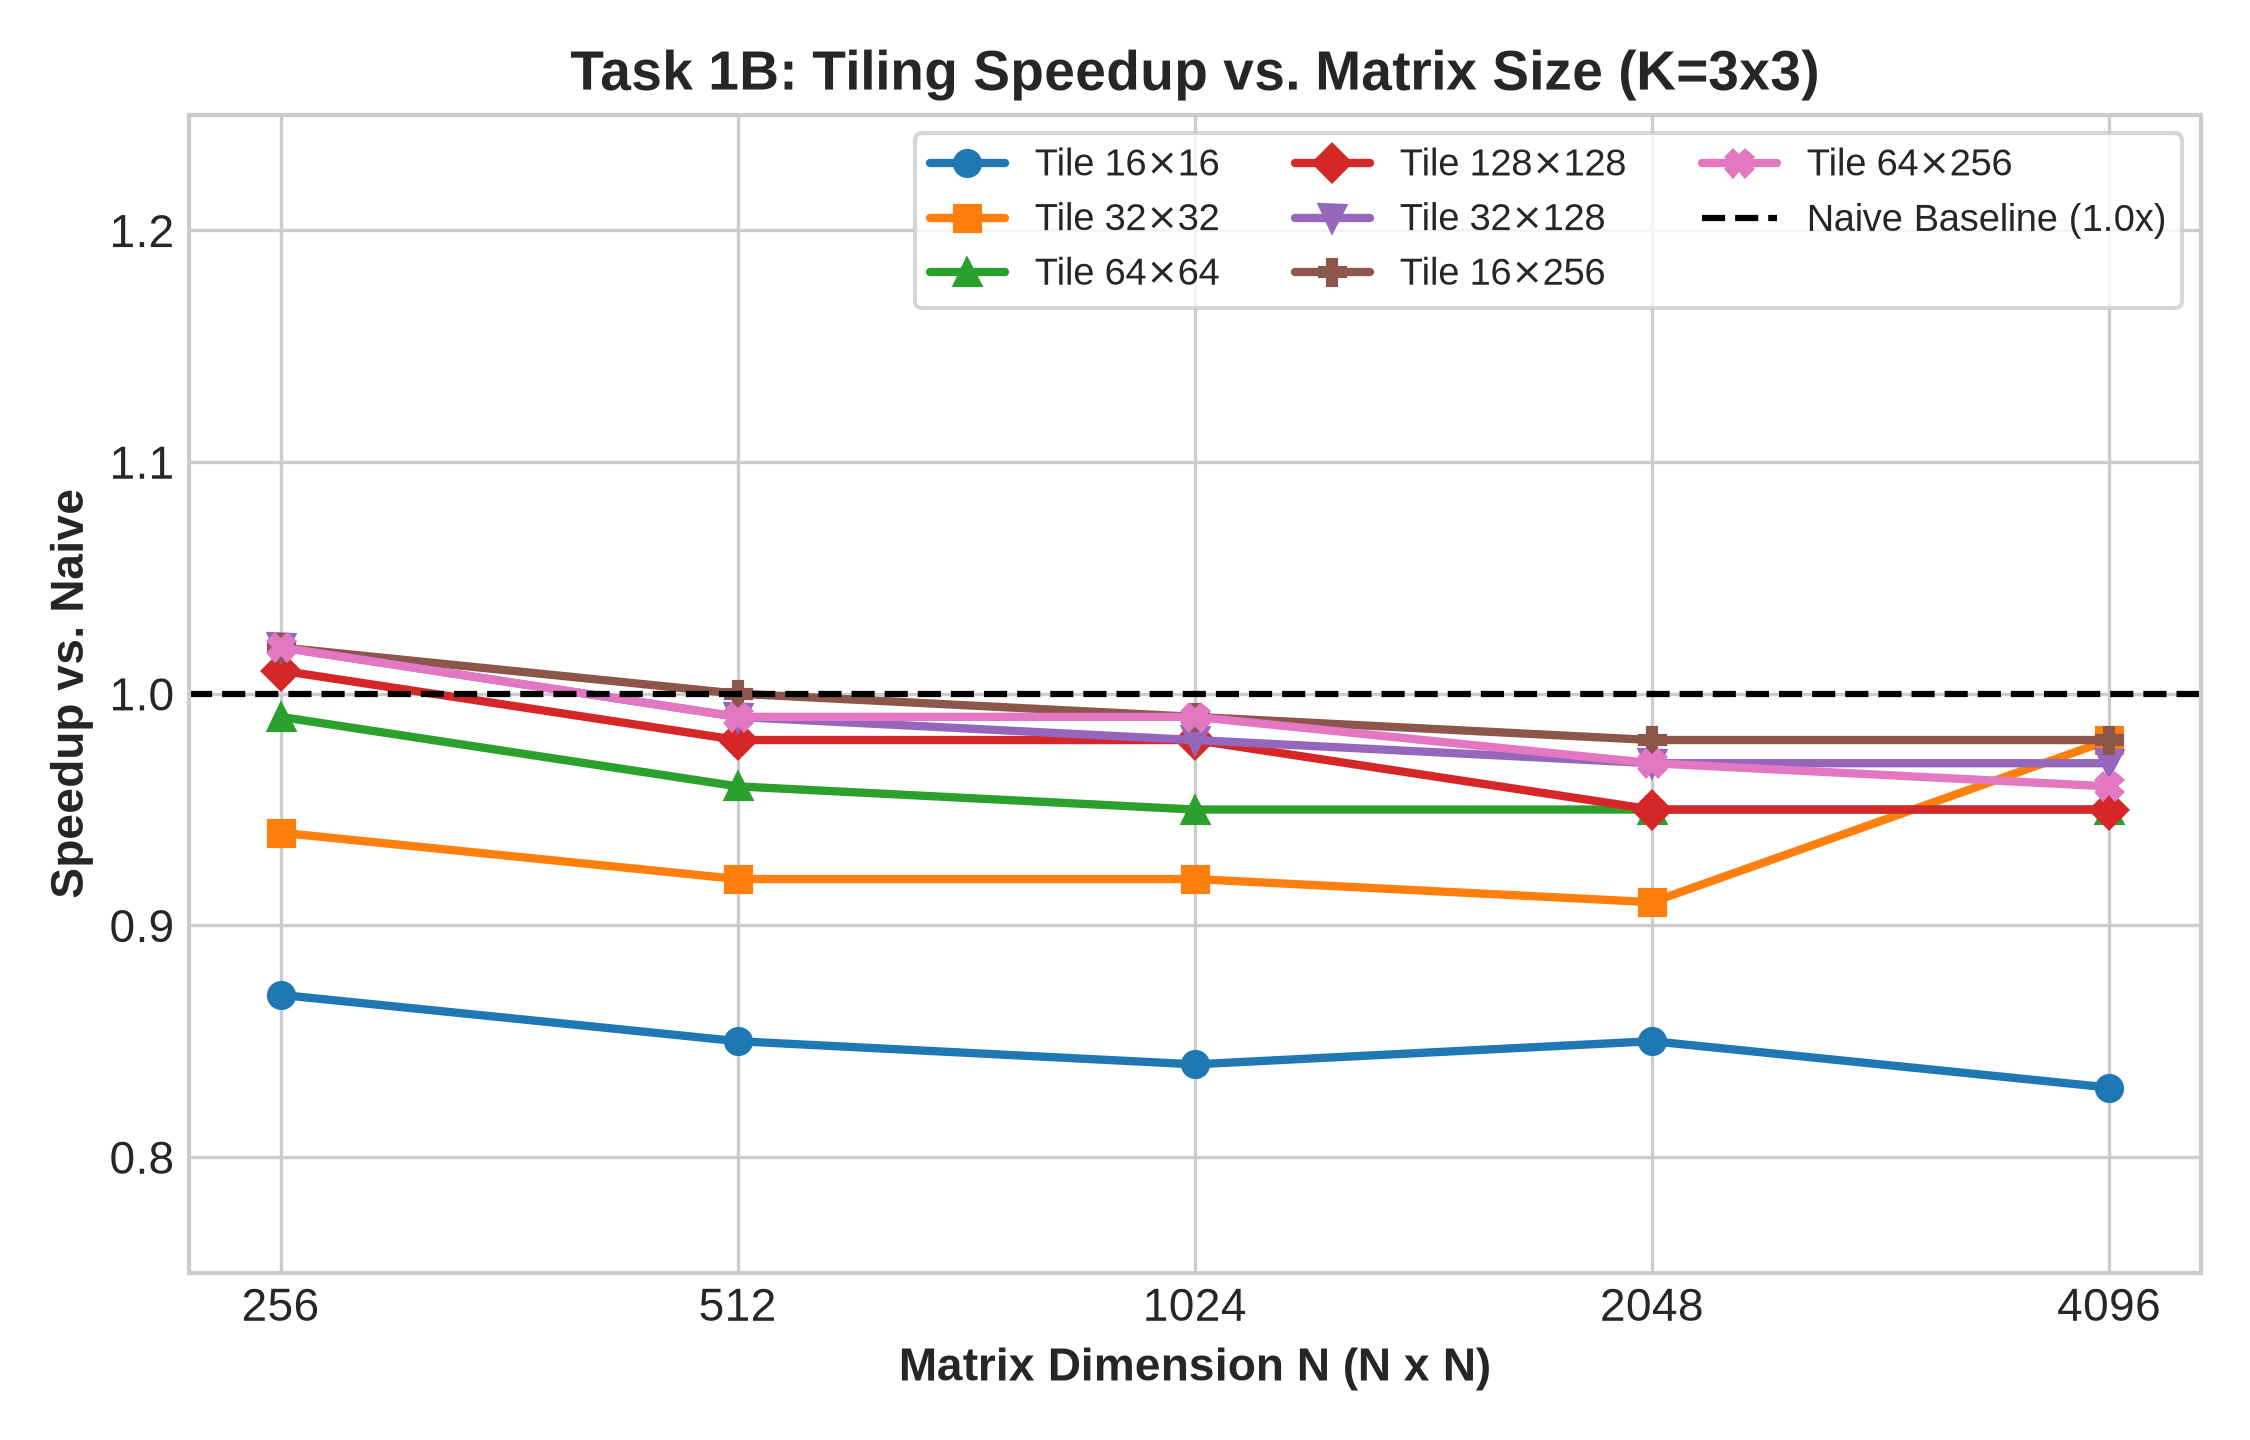
\includegraphics[width=\textwidth]{figures/1b_speedup_matrix_k3.png}\\
        {\small (a) Tiling Speedup vs. Matrix Size ($K=3$)}
    \end{minipage}
    \hfill
    \begin{minipage}{0.48\textwidth}
        \centering
        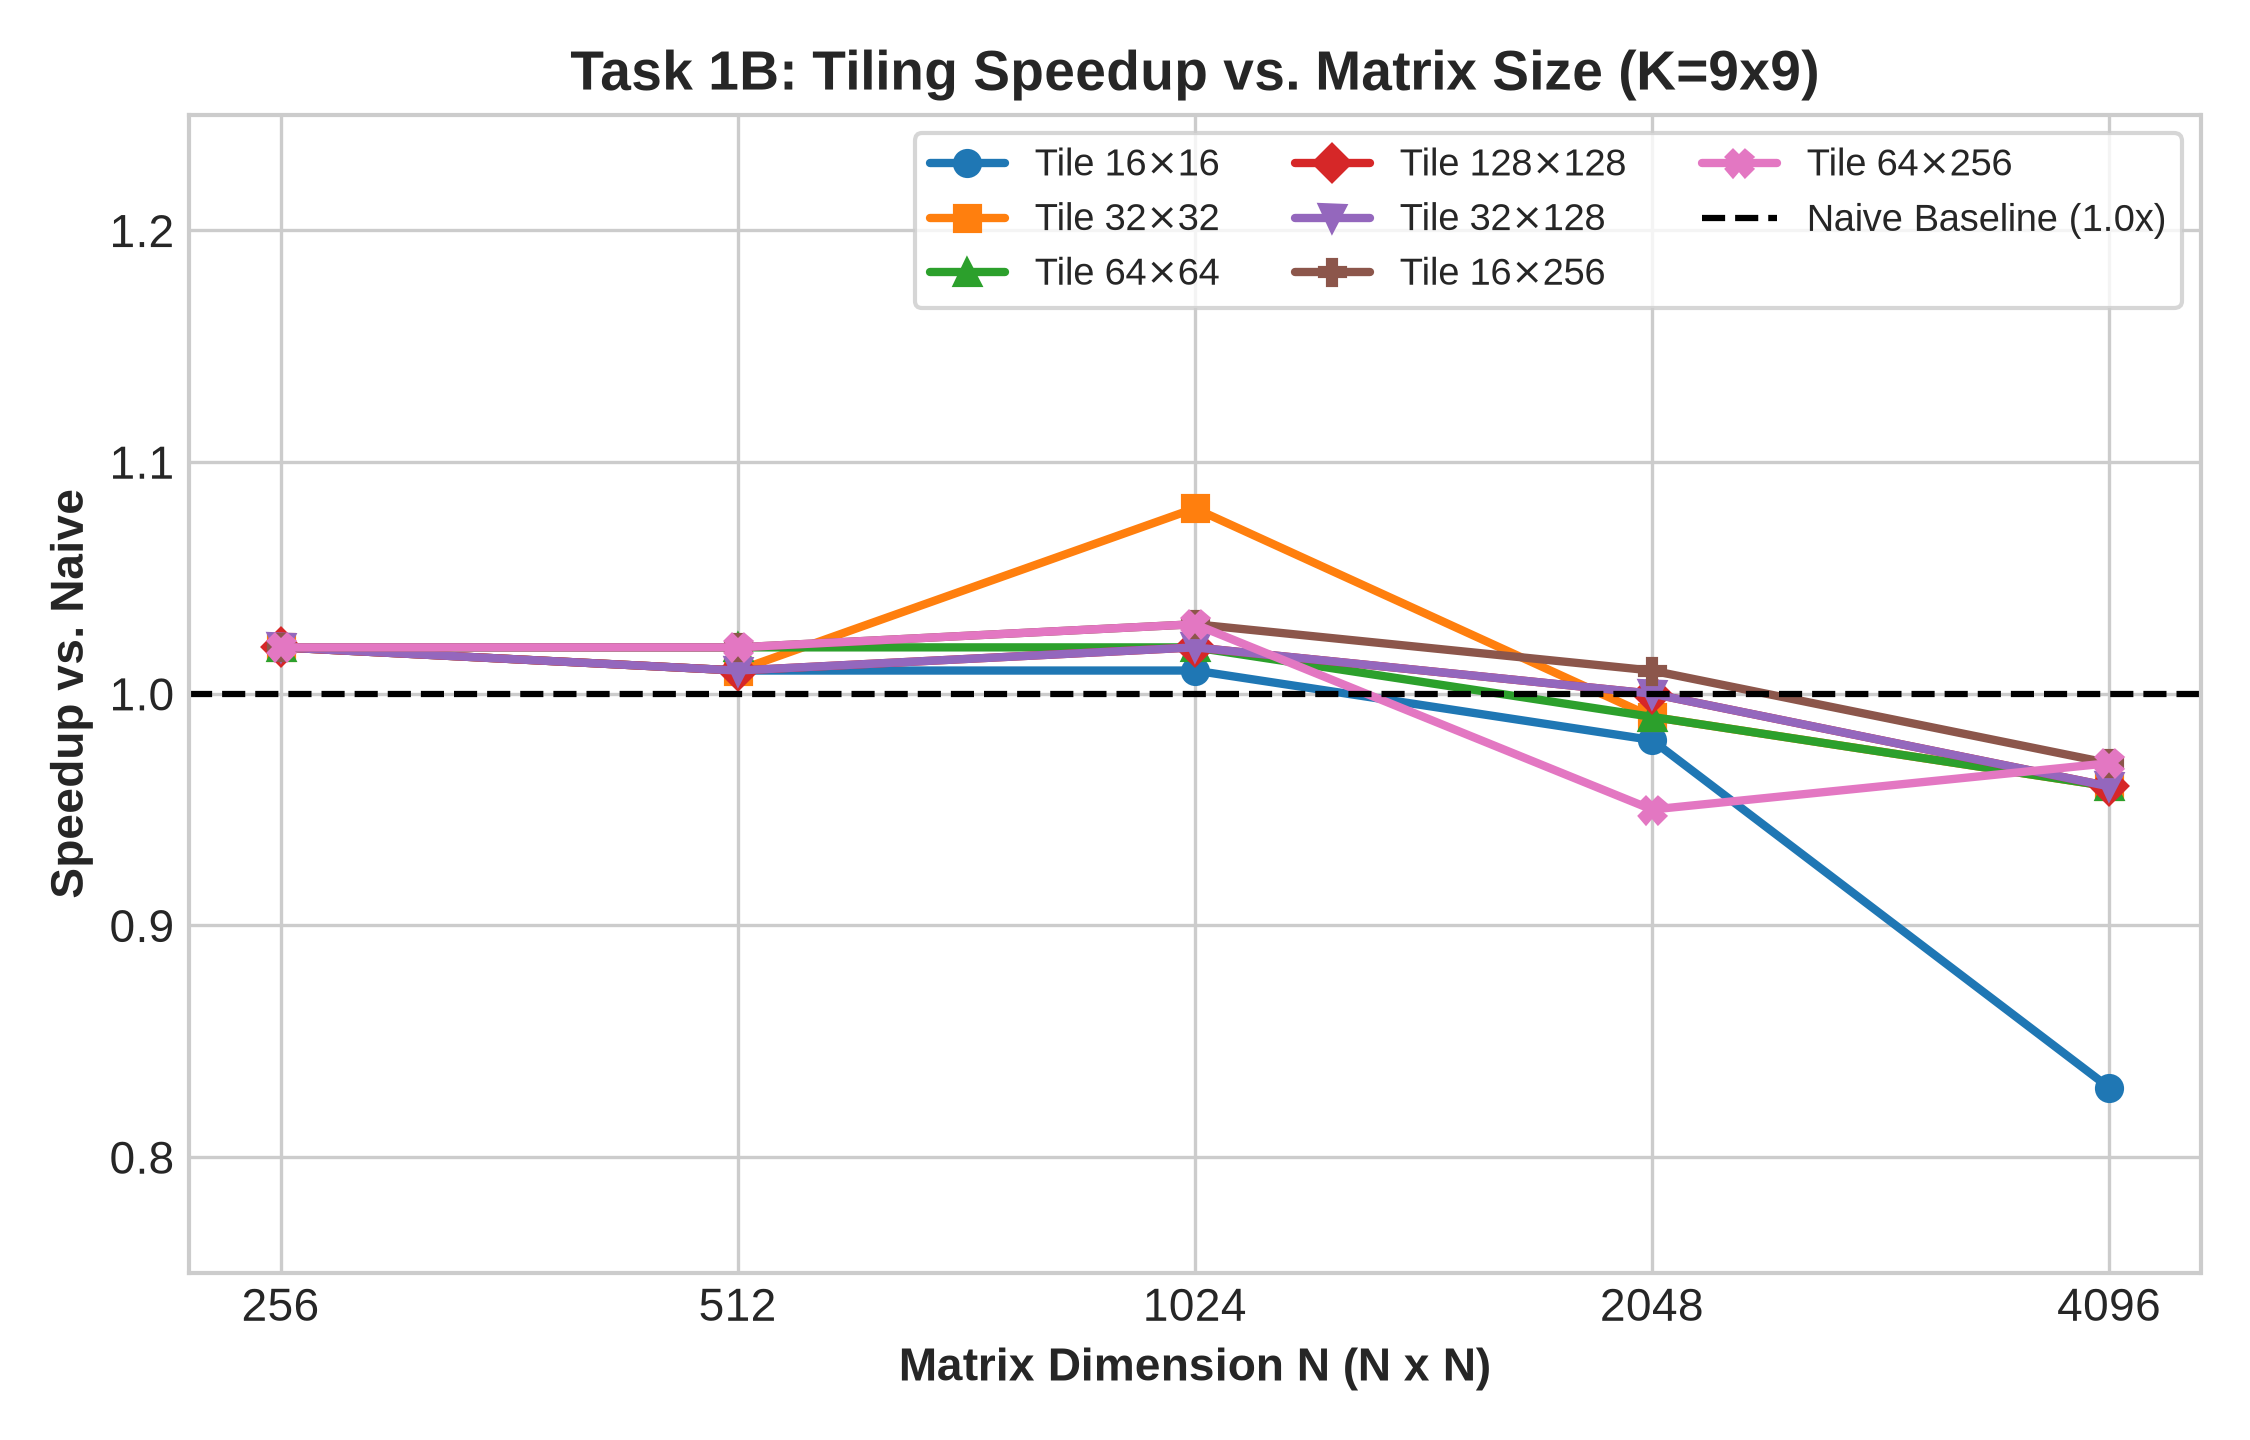
\includegraphics[width=\textwidth]{figures/1b_speedup_matrix_k9.png}\\
        {\small (b) Tiling Speedup vs. Matrix Size ($K=9$)}
    \end{minipage}
    \caption{Task 1B: Performance Evaluation Across Cache Tiling Configurations.}
    \label{fig:1b_tiling_plots}
\end{figure}

\begin{figure}[h!]
    \centering
    \begin{minipage}{0.48\textwidth}
        \centering
        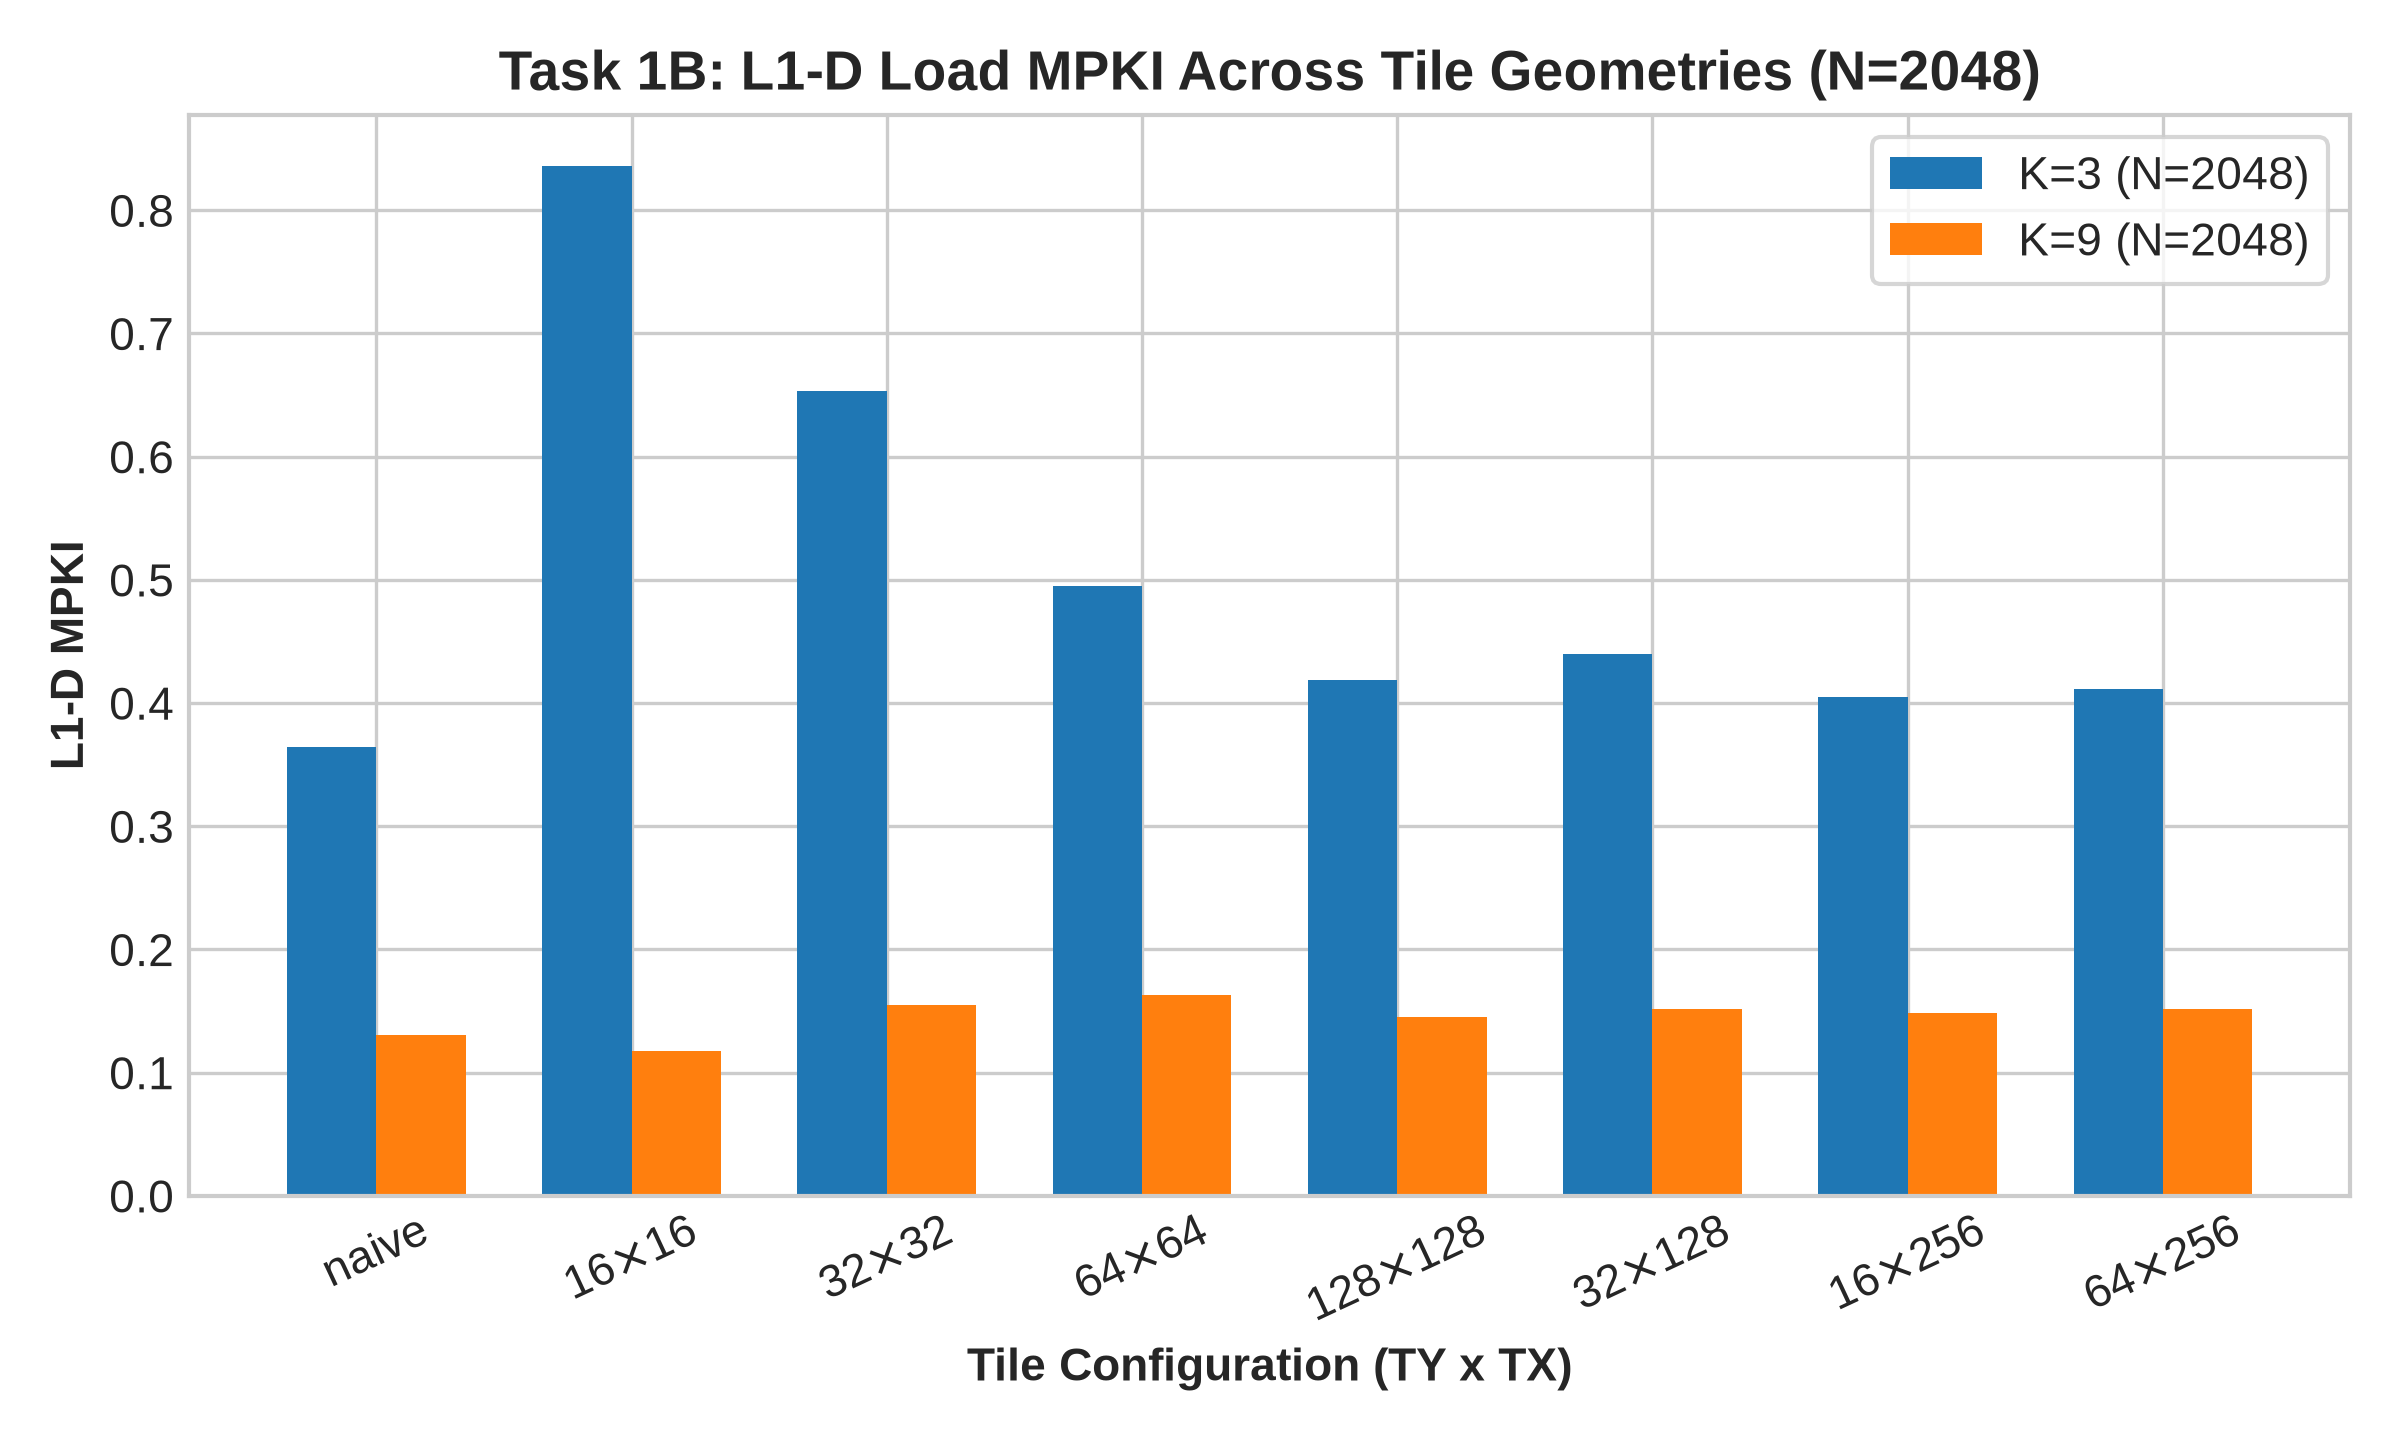
\includegraphics[width=\textwidth]{figures/1b_l1_miss_rate_comparison.png}\\
        {\small (a) L1-D Miss Rate Comparison}
    \end{minipage}
    \hfill
    \begin{minipage}{0.48\textwidth}
        \centering
        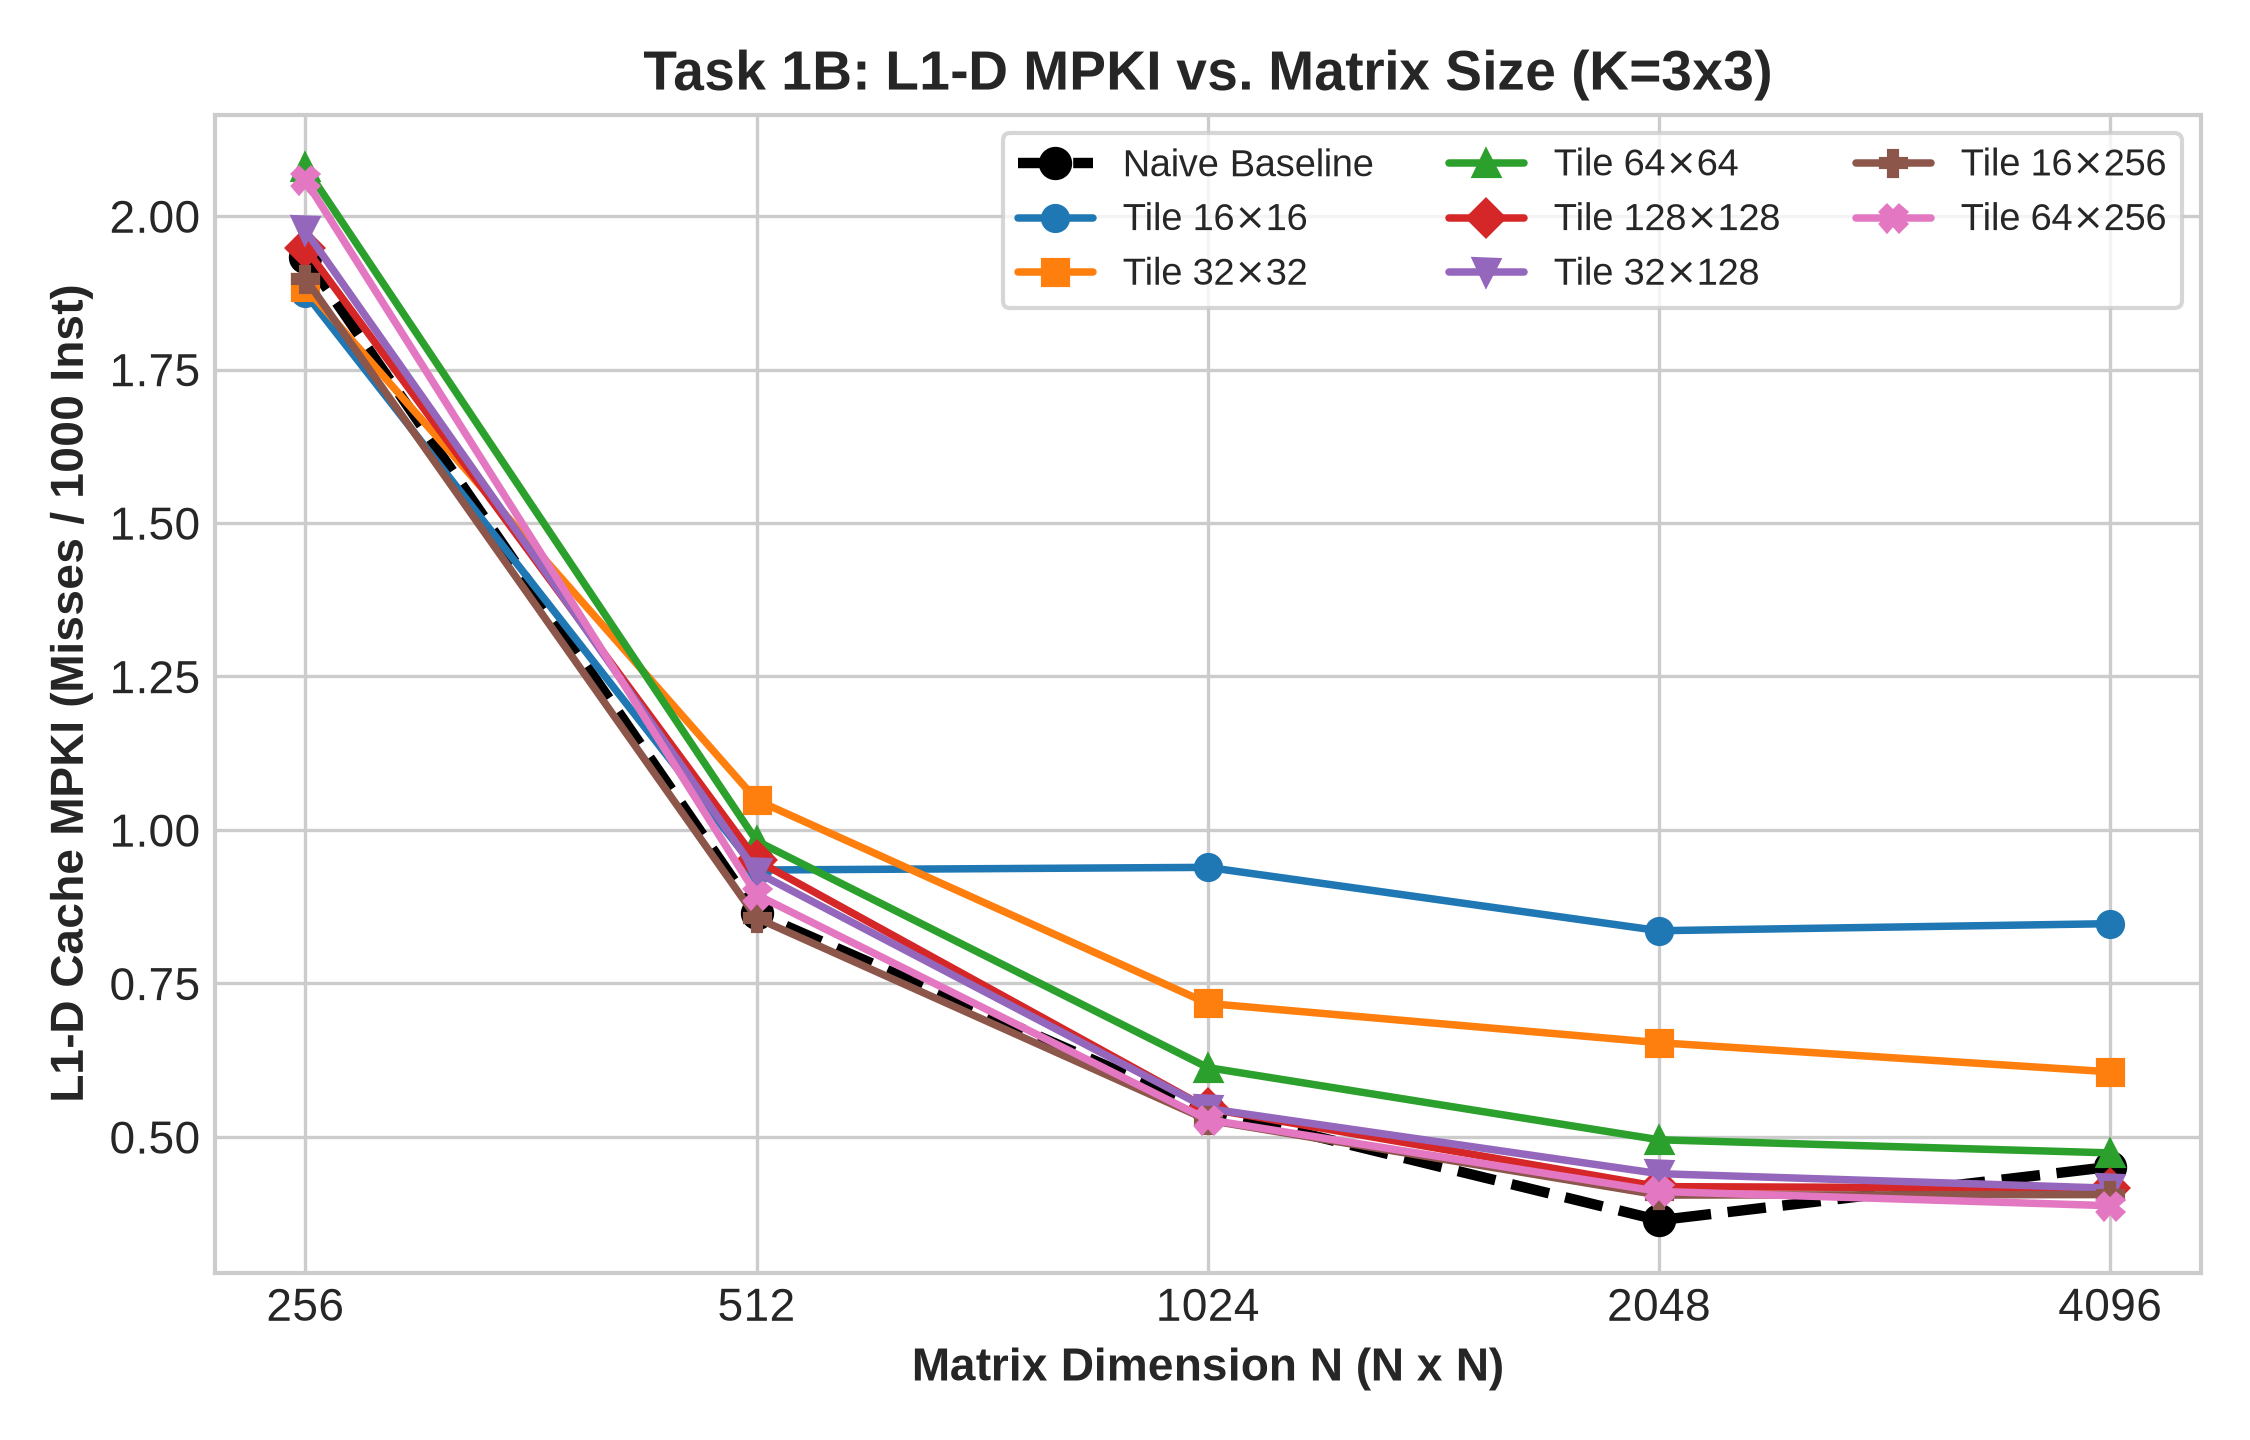
\includegraphics[width=\textwidth]{figures/1b_l1_mpki_matrix_k3.png}\\
        {\small (b) L1-D MPKI Comparison ($K=3$)}
    \end{minipage}
    \caption{Task 1B: Cache Memory Hierarchy Behavior Under Tiling.}
    \label{fig:1b_tiling_metrics}
\end{figure}



\subsubsection{Question 1: L1D-MPKI Tiling vs Naive }
\begin{itemize}
    \item There is no clear pattern, in some configurations MPKI decreased but in most cases it increases leading to negative speedup
    \item The L1D miss rate is $< 0.5\%$ so tiling isn't really helping, worser performance due to constant factors 
\end{itemize}

\subsubsection{Question 2: L1-D MPKI Variation Across Matrix Sizes and Tile Sizes}
\begin{itemize}
    \item \textbf{Variation Across Matrix Sizes ($N$)}:
    \begin{itemize}
        \item L1D-MPKI steadily decreased with Matrix Size 
        \item \textbf At small $N$, cold compulsory misses dominate per instruction. At large $N$, the working set fits in cache keeping the MPKI small
    \end{itemize}
    \item \textbf{Variation Across Tile Sizes}:
    \begin{itemize}
        \item For K=3, there is a decreasing pattern of L1-D MPKI but there is no clear pattern for K=9
        \item The general decreasing pattern is due to better utilization of L1D cache 
    \end{itemize}
\end{itemize}

\subsubsection{Question 3: Speedup Evaluation, Limiting Factors, and Proposed Solutions}
\begin{itemize}
    \item \textbf{Speedup Quantification}:
    \begin{itemize}
        \item Tiling alone yields \textbf{no significant speedup}, fluctuating tightly between \textbf{$0.83\times$ and $1.02\times$} across all workloads.
        % \item Undersized tiles ($16\times 16$) incur a $\sim 17\%$ slowdown ($0.83\times$--$0.85\times$); calibrated tiles ($32\times 128$) achieve parity ($0.97\times$--$1.02\times$).
    \end{itemize}
    \item \textbf{Limiting Factors}:
    \begin{itemize}
        \item Unlike matrix multiplication where reuse scales as $O(N)$, 2D convolution data reuse is capped at $K^2$. The active rows already fit in the cache in naive code, hence tiling isn't improving
        % \item \textbf{Serial FMA Pipeline Latency}: Scalar convolution is bound by the \textbf{4-cycle serial arithmetic latency chain} on a single accumulator. Tiling rearranges cache addresses but does not break this instruction dependency chain.
        % \item \textbf{Loop Control Overhead}: Adding two outer tiling loops increases total  instructions by $2\%$--$5\%$ without performing useful computation.
    \end{itemize}
    \item \textbf{Proposed Solution}:
    \begin{itemize}
        \item Combine cache tiling with \textbf{AVX2 SIMD} (to execute 8 FMAs per cycle), so cache usage becomes more, as implemented in Task 1D.
    \end{itemize}
\end{itemize}

% \clearpage
\section{Task 1C: SIMD Vectorization Optimization (\texttt{conv\_simd})}
\subsection{Deliverables}
\noindent \textbf{1. Baseline Profiling}
\begin{itemize}
    \item Instructions : 667.59M
    % \item \textbf{Baseline Instruction Burden}: Scalar 2D convolution requires $W \times K^2$ individual scalar loads, address calculations, scalar FMA operations, and loop branch tests per row, totaling $667.59\times 10^6$ instructions for $N=2048, K=3$ and $2707.34\times 10^6$ for $K=9$.
        
\end{itemize}
\noindent \textbf{3. Instruction Count and Performance Analysis}
\textbf{SIMD Implementations}:
    \begin{itemize}
        \item \textbf{128-bit SIMD (\texttt{conv\_simd128})}: Utilizes Intel SSE/AVX 128-bit vector registers (\texttt{\_\_m128}) to process 4 single-precision floating-point numbers concurrently per vector operation.
        \begin{itemize}
            \item Instructions: 371.71M
            \item Speedup: 4.06x
        \end{itemize}
        \item \textbf{256-bit SIMD (\texttt{conv\_simd256})}: Utilizes Intel AVX2 256-bit vector registers (\texttt{\_\_m256}) to process 8 single-precision floating-point numbers concurrently per vector operation.
        \begin{itemize}
            \item Instructions: 328.82M
            \item Speedup: 7.81x
        \end{itemize}
        \item \textbf{512-bit SIMD} is not supported on my Laptop
    \end{itemize}


\noindent \textbf{4. Multi-Size Evaluation}\\ \\
Table~\ref{tab:1c_simd} summarizes the execution time, speedup,  instruction counts, cycles, IPC, L1-D miss rates, and L1-D MPKI across all evaluated matrix sizes ($N \in \{256, 512, 1024, 2048, 4096\}$) and kernel sizes ($K \in \{3, 9\}$).

{\footnotesize
\setlength{\tabcolsep}{3.5pt}
\begin{longtable}{rrcrrrrrrr}
\caption{Task 1C: Performance and Hardware Counters for SIMD Vectorization (128-bit \& 256-bit) vs. Naive Baseline} \label{tab:1c_simd} \\
\toprule
$K$ & $N$ & Configuration & Time & Speedup &  Instructions & Cycles & IPC & L1-D Miss & L1-D \\
    &     &               & (ms) &         & ($\times 10^6$) & ($\times 10^6$) &     & Rate & MPKI \\
\midrule
\endfirsthead

\multicolumn{10}{c}{{\bfseries Table \thetable\ Continued from previous page}} \\
\toprule
$K$ & $N$ & Configuration & Time & Speedup &  Instructions & Cycles & IPC & L1-D Miss & L1-D \\
    &     &               & (ms) &         & ($\times 10^6$) & ($\times 10^6$) &     & Rate & MPKI \\
\midrule
\endhead

\midrule
\multicolumn{10}{r}{{Continued on next page\dots}} \\
\endfoot

\bottomrule
\endlastfoot

3 & 256 & naive & 0.311 & 1.00$\times$ & 13.56 & 5.15 & 2.63 & 1.42\% & 2.67 \\
3 & 256 & simd128 (SSE) & 0.069 & \textbf{4.51$\times$} & 8.91 & 4.61 & 1.93 & 1.56\% & 2.90 \\
3 & 256 & simd256 (AVX2) & 0.036 & \textbf{8.64$\times$} & 8.24 & 4.48 & 1.84 & 1.71\% & 3.13 \\
\midrule
3 & 512 & naive & 1.122 & 1.00$\times$ & 44.73 & 13.29 & 3.37 & 0.54\% & 0.94 \\
3 & 512 & simd128 (SSE) & 0.268 & \textbf{4.19$\times$} & 26.20 & 10.21 & 2.57 & 0.93\% & 1.51 \\
3 & 512 & simd256 (AVX2) & 0.129 & \textbf{8.70$\times$} & 23.41 & 9.70 & 2.41 & 1.08\% & 1.68 \\
\midrule
3 & 1024 & naive & 4.461 & 1.00$\times$ & 168.85 & 44.98 & 3.75 & 0.29\% & 0.49 \\
3 & 1024 & simd128 (SSE) & 1.055 & \textbf{4.23$\times$} & 94.92 & 32.97 & 2.88 & 0.59\% & 0.92 \\
3 & 1024 & simd256 (AVX2) & 0.503 & \textbf{8.87$\times$} & 84.17 & 31.29 & 2.69 & 0.74\% & 1.07 \\
\midrule
3 & 2048 & naive & 17.797 & 1.00$\times$ & 667.59 & 180.68 & 3.69 & 0.21\% & 0.35 \\
3 & 2048 & simd128 (SSE) & 4.387 & \textbf{4.06$\times$} & 371.71 & 133.92 & 2.78 & 0.46\% & 0.69 \\
3 & 2048 & simd256 (AVX2) & 2.278 & \textbf{7.81$\times$} & 328.82 & 125.37 & 2.62 & 0.57\% & 0.81 \\
\midrule
3 & 4096 & naive & 71.334 & 1.00$\times$ & 2670.81 & 703.13 & 3.80 & 0.23\% & 0.39 \\
3 & 4096 & simd128 (SSE) & 17.889 & \textbf{3.99$\times$} & 1488.09 & 508.25 & 2.93 & 0.50\% & 0.75 \\
3 & 4096 & simd256 (AVX2) & 9.806 & \textbf{7.27$\times$} & 1315.27 & 484.29 & 2.72 & 0.65\% & 0.92 \\
\midrule
9 & 256 & naive & 2.459 & 1.00$\times$ & 45.52 & 13.35 & 3.41 & 0.23\% & 0.62 \\
9 & 256 & simd128 (SSE) & 0.751 & \textbf{3.27$\times$} & 15.78 & 7.11 & 2.22 & 0.70\% & 1.79 \\
9 & 256 & simd256 (AVX2) & 0.376 & \textbf{6.54$\times$} & 11.69 & 5.60 & 2.09 & 0.95\% & 2.19 \\
\midrule
9 & 512 & naive & 9.785 & 1.00$\times$ & 172.23 & 45.60 & 3.78 & 0.10\% & 0.25 \\
9 & 512 & simd128 (SSE) & 2.985 & \textbf{3.28$\times$} & 53.38 & 20.24 & 2.64 & 0.34\% & 0.87 \\
9 & 512 & simd256 (AVX2) & 1.504 & \textbf{6.51$\times$} & 37.02 & 14.54 & 2.55 & 0.45\% & 1.02 \\
\midrule
9 & 1024 & naive & 39.016 & 1.00$\times$ & 678.88 & 171.88 & 3.95 & 0.05\% & 0.14 \\
9 & 1024 & simd128 (SSE) & 11.934 & \textbf{3.27$\times$} & 203.66 & 73.50 & 2.77 & 0.20\% & 0.51 \\
9 & 1024 & simd256 (AVX2) & 6.015 & \textbf{6.49$\times$} & 138.49 & 50.83 & 2.72 & 0.28\% & 0.63 \\
\midrule
9 & 2048 & naive & 151.971 & 1.00$\times$ & 2707.34 & 673.27 & 4.02 & 0.04\% & 0.12 \\
9 & 2048 & simd128 (SSE) & 47.779 & \textbf{3.18$\times$} & 808.32 & 299.79 & 2.70 & 0.17\% & 0.43 \\
9 & 2048 & simd256 (AVX2) & 24.098 & \textbf{6.31$\times$} & 546.29 & 207.94 & 2.63 & 0.27\% & 0.61 \\
\midrule
9 & 4096 & naive & 592.072 & 1.00$\times$ & 10832.44 & 2627.20 & 4.12 & 0.05\% & 0.12 \\
9 & 4096 & simd128 (SSE) & 191.157 & \textbf{3.10$\times$} & 3228.33 & 1194.30 & 2.70 & 0.16\% & 0.42 \\
9 & 4096 & simd256 (AVX2) & 135.740 & \textbf{4.36$\times$} & 2186.83 & 835.33 & 2.62 & 0.28\% & 0.63 \\
\midrule
\end{longtable}
}

\begin{figure}[h!]
    \centering
    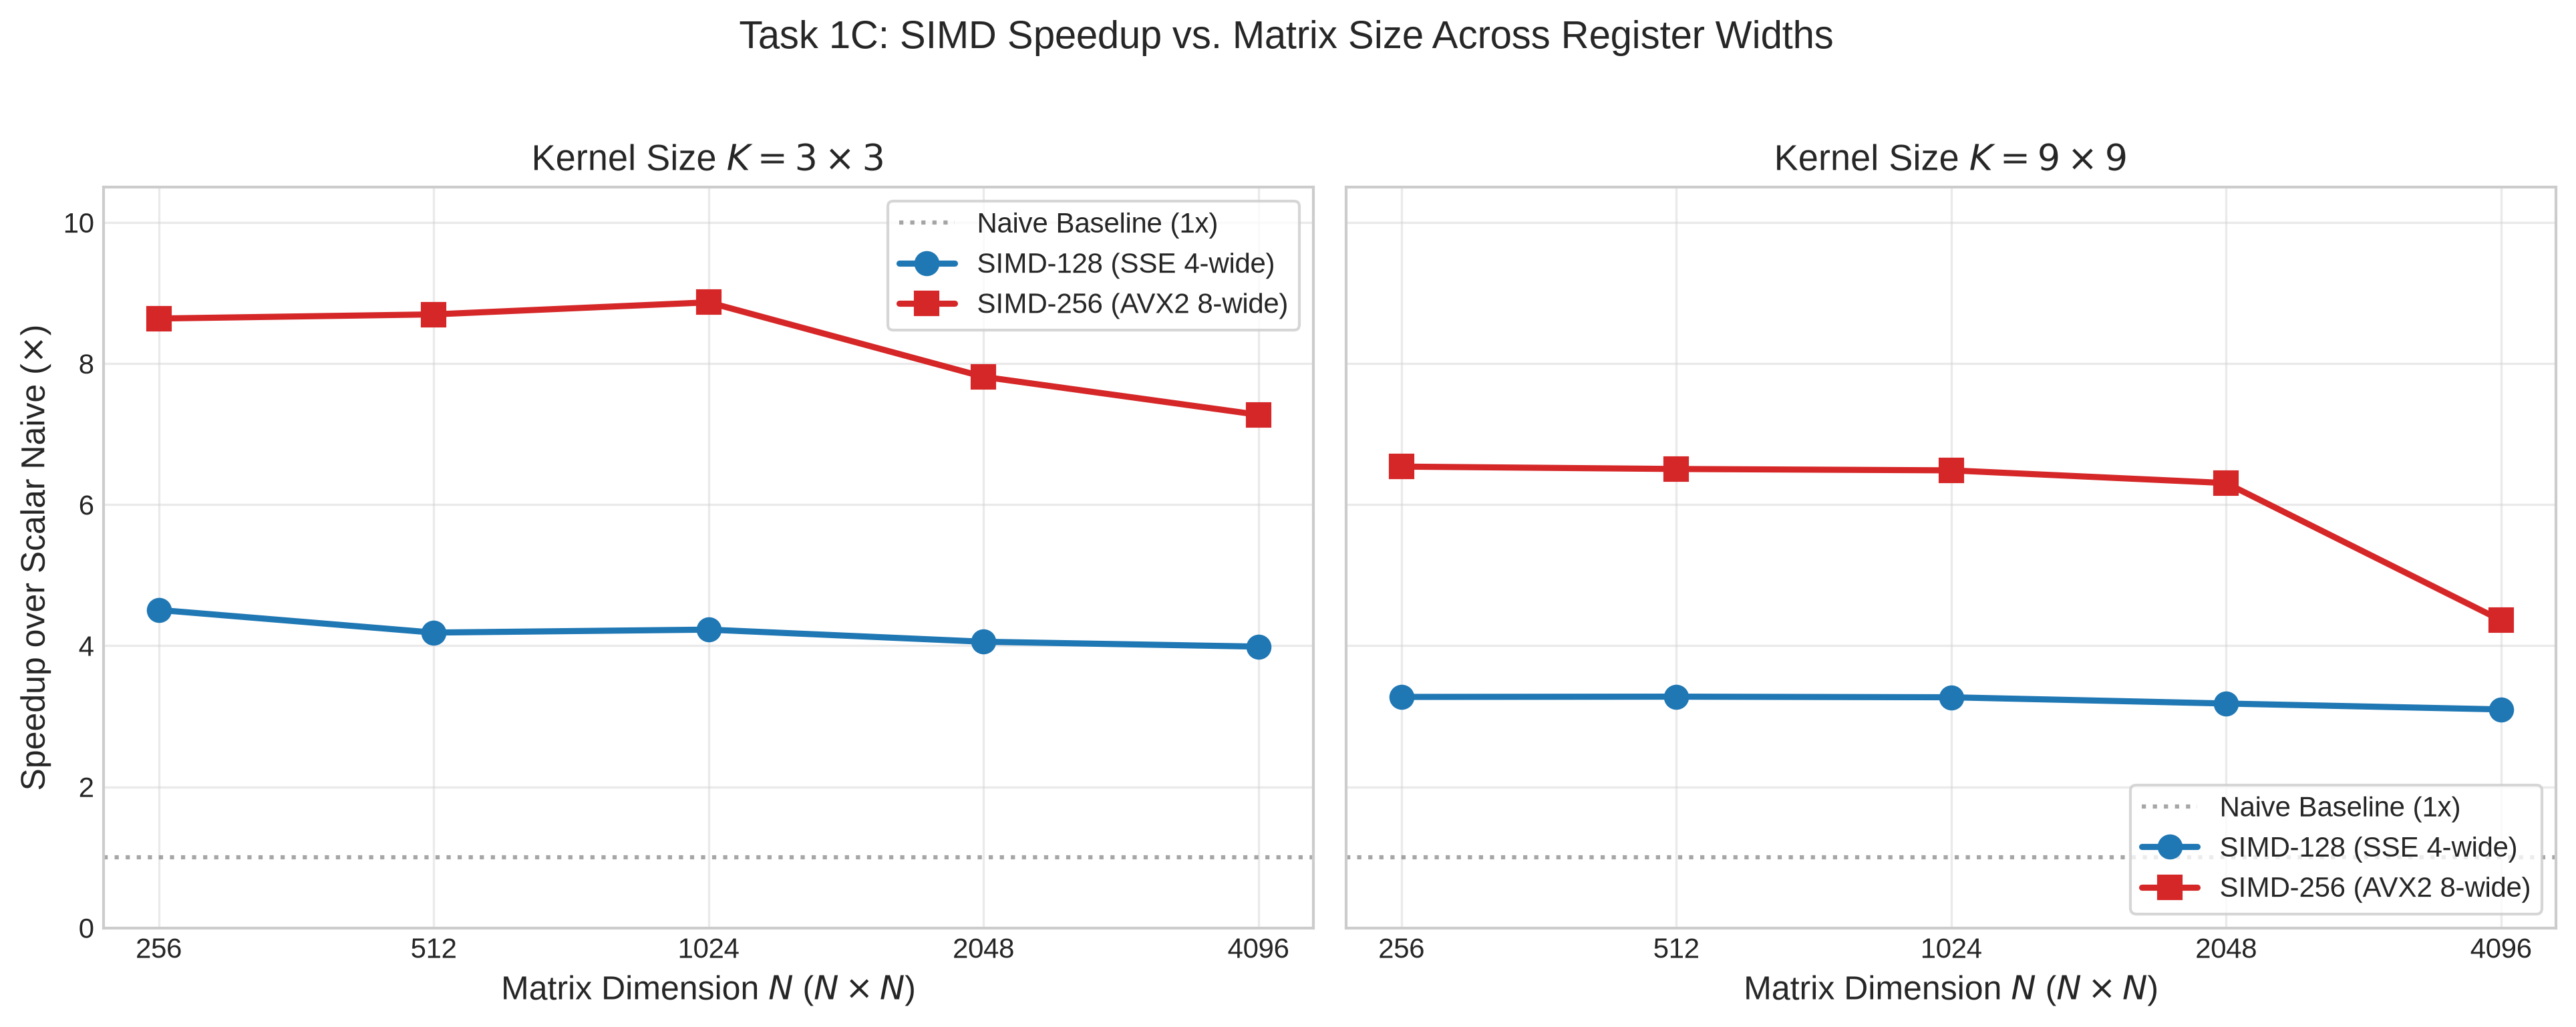
\includegraphics[width=\textwidth]{figures/1c_simd_speedup.png}
    \caption{Task 1C: Speedup over Scalar Naive Baseline across Matrix Sizes for SIMD-128 (SSE) and SIMD-256 (AVX2).}
    \label{fig:1c_speedup}
\end{figure}

\begin{figure}[h!]
    \centering
    \begin{minipage}{0.80\textwidth}
        \centering
        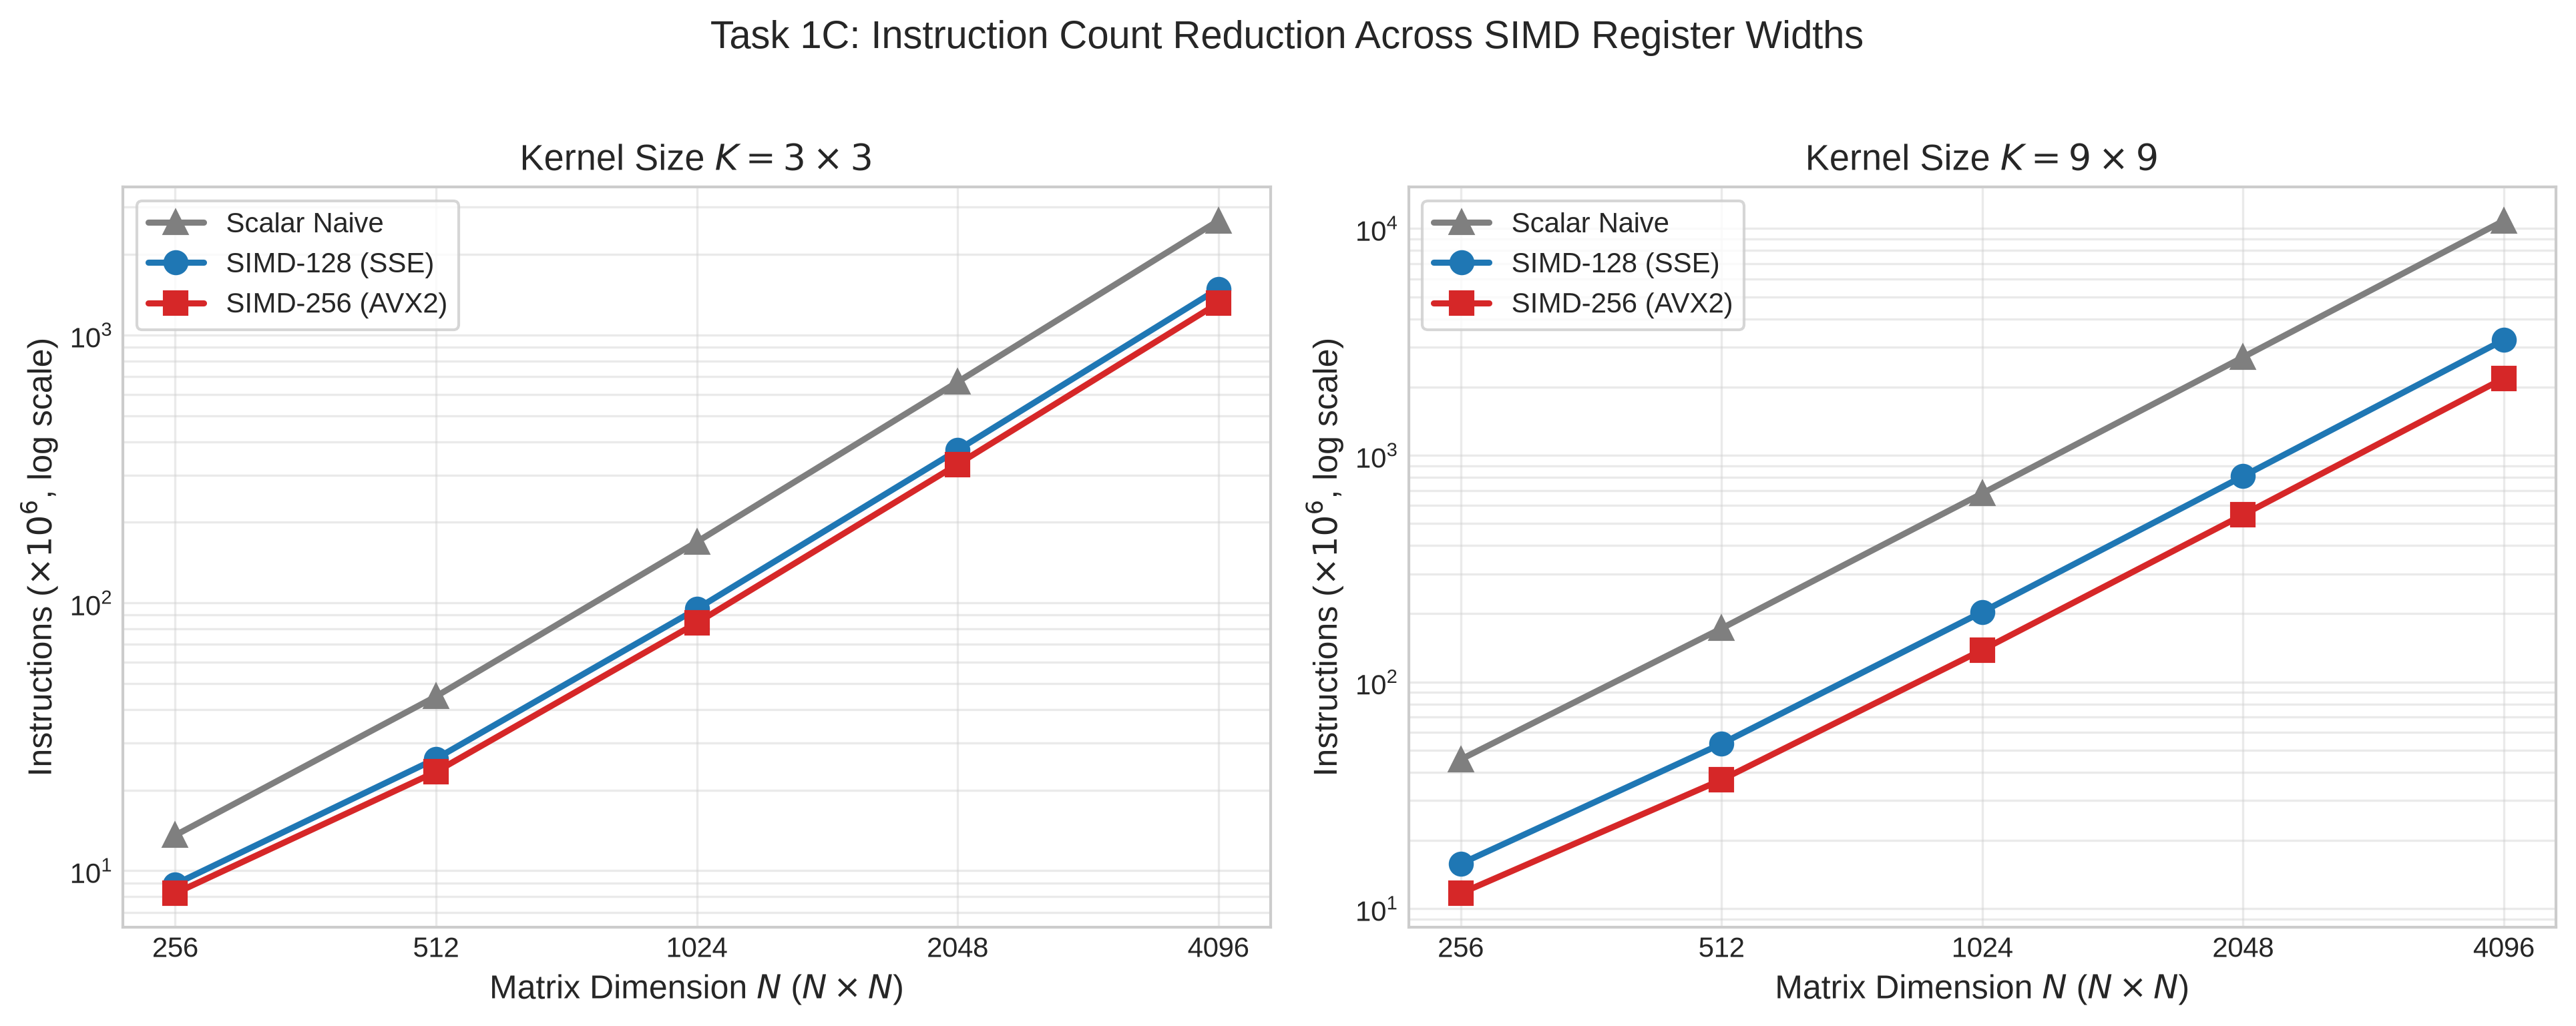
\includegraphics[width=\textwidth]{figures/1c_simd_instructions.png}\\
        {\small (a)  Instructions Reduction Across Register Widths}
    \end{minipage}
    % \hfill
    % \begin{minipage}{0.48\textwidth}
    %     \centering
    %     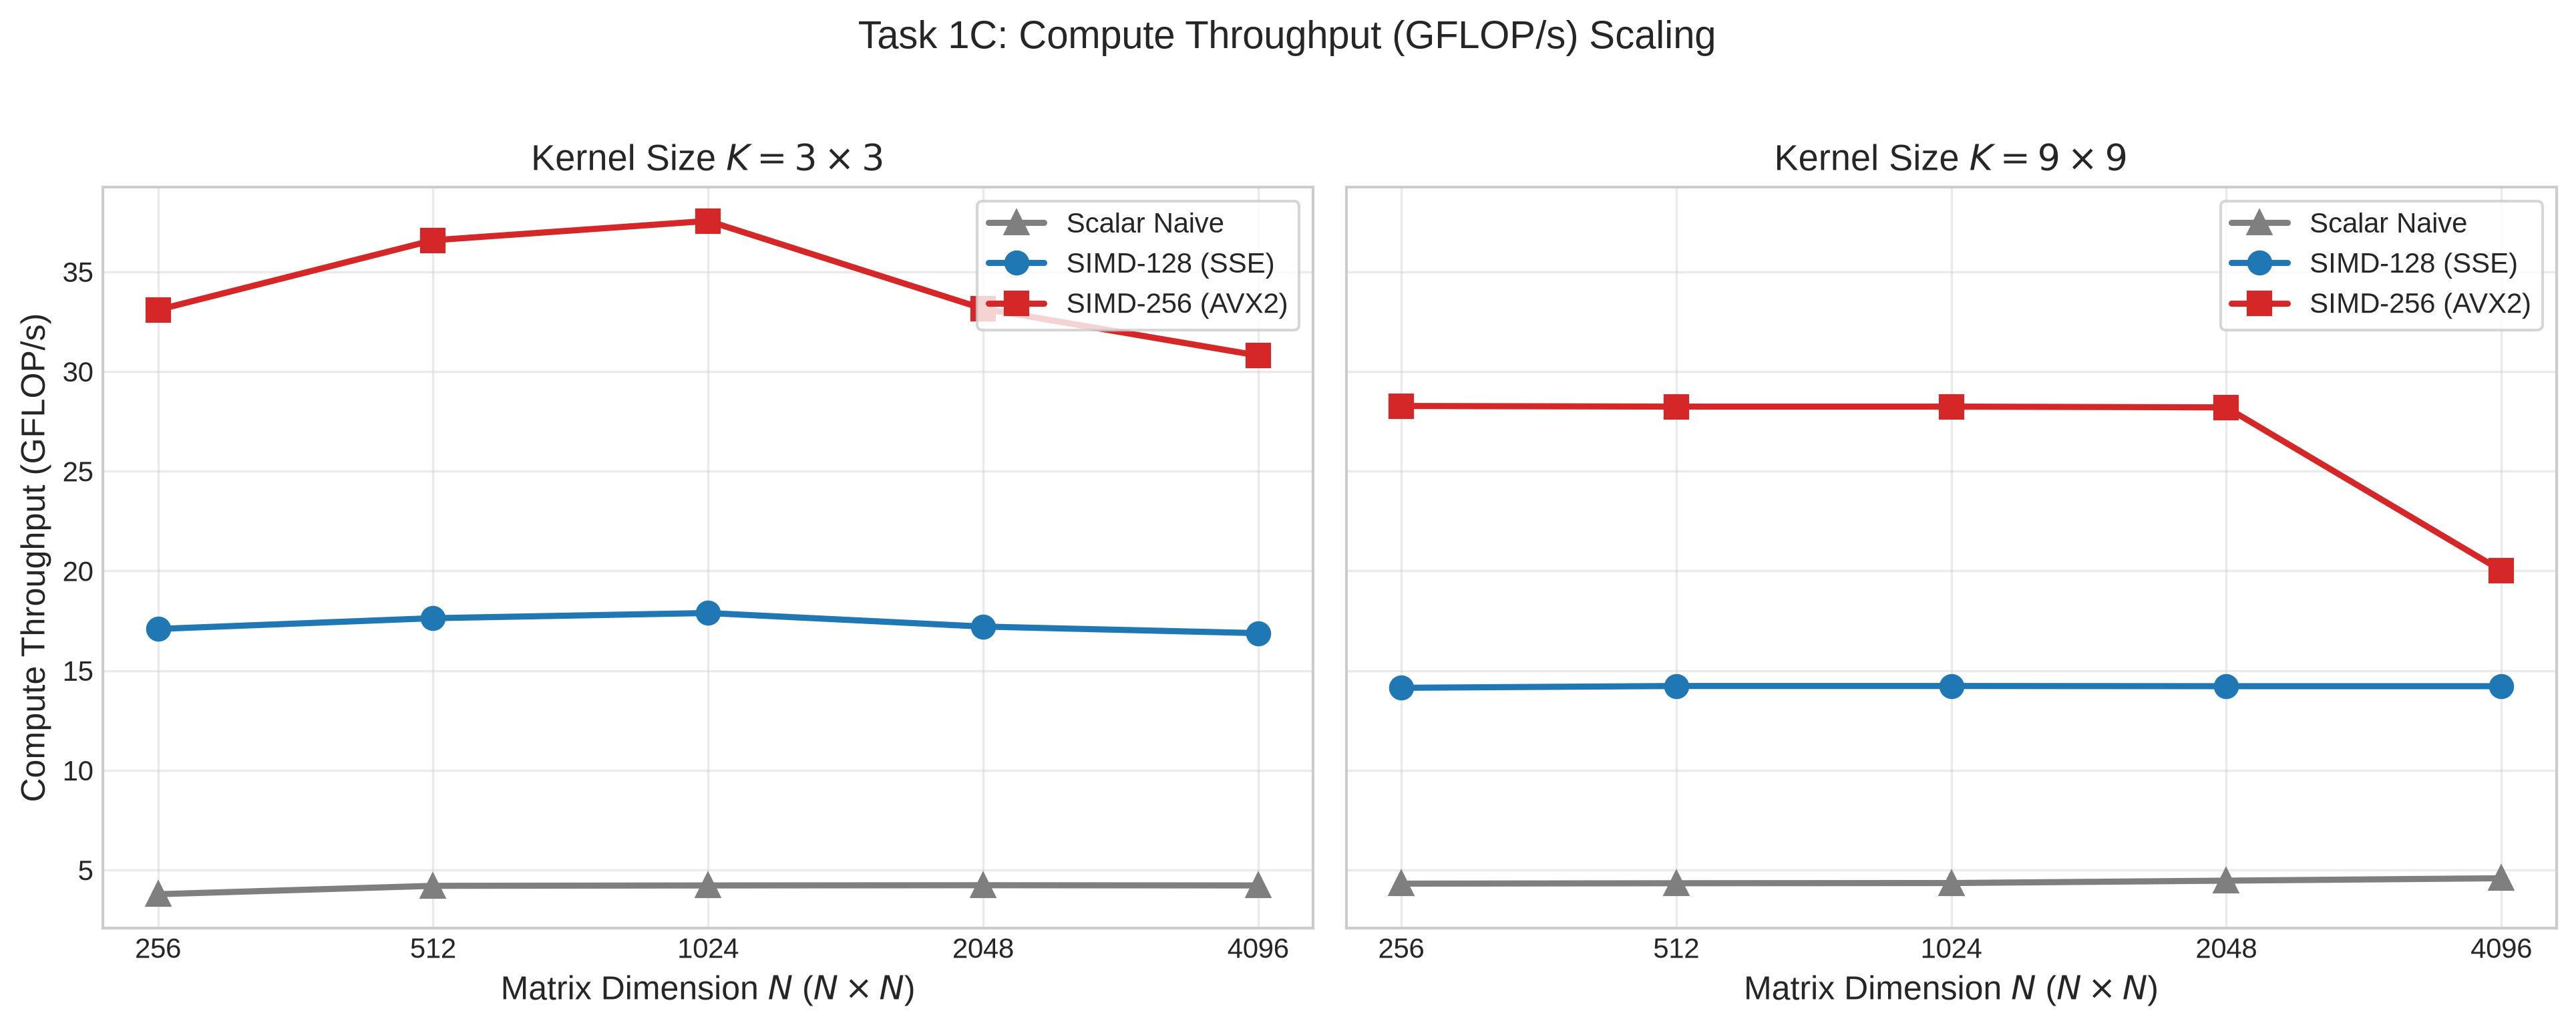
\includegraphics[width=\textwidth]{figures/1c_simd_gflops.png}\\
    %     {\small (b) Compute Throughput (GFLOP/s) Scaling}
    % \end{minipage}
    \caption{Task 1C: Microarchitectural Impact of SIMD Vectorization.}
    \label{fig:1c_metrics}
\end{figure}


\subsubsection{Question 1: Change in Number of Instructions from Naive to SIMD Implementation}
\begin{itemize}
    \item \textbf{Observed Changes}:
    \begin{itemize}
        \item \textbf{SIMD-128 (SSE)}: Reduces  instructions by \textbf{44.3\% to 70.1\%} compared to naive baseline (e.g., at $N=2048, K=3$: $667.59\times 10^6 \to 371.71\times 10^6$ [$-44.3\%$]; at $K=9$: $2707.34\times 10^6 \to 808.32\times 10^6$ [$-70.1\%$]).
        \item \textbf{SIMD-256 (AVX2)}: Reduces  instructions by \textbf{50.8\% to 79.8\%} compared to naive baseline (e.g., at $N=2048, K=3$: $667.59\times 10^6 \to 328.82\times 10^6$ [$-50.8\%$]; at $K=9$: $2707.34\times 10^6 \to 546.29\times 10^6$ [$-79.8\%$]).
    \end{itemize}
    \item \textbf{Justifications}:
    \begin{itemize}
        \item Since SIMD is packing some instructions into packs of 4 or 8, the total instructions reduces
        \item Number of iterations of innermost loop reduces hence number of branch conditional instructions reduces
        % \item \textbf{Vectorized Arithmetic Packing}: In scalar naive, calculating $W$ output pixels along a row requires issuing $W \times K^2$ distinct scalar multiplications and additions. SIMD packs 4 (128-bit) or 8 (256-bit) adjacent horizontal pixels into a single vector lane, reducing the total arithmetic instruction count by up to $4\times$ and $8\times$.
        % \item \textbf{Loop Branch Control Elimination}: Stepping the innermost loop by 4 (\texttt{ox += 4}) or 8 (\texttt{ox += 8}) reduces loop boundary condition evaluations, index increments, and conditional branch jumps by $75\%$ and $87.5\%$ respectively.
        % \item \textbf{FMA Instruction Fusion}: Utilizing Fused Multiply-Add (\texttt{\_mm\_fmadd\_ps} / \texttt{\_mm256\_fmadd\_ps}) executes floating-point multiplication and addition in a single  instruction cycle rather than separate \texttt{vmulps} and \texttt{vaddps} instructions.
    \end{itemize}
\end{itemize}

\subsubsection{Question 2: Speedup Evaluation, Contributing Factors}
\begin{itemize}
    \item \textbf{Speedup Quantification}:
    \begin{itemize}
        \item \textbf{SIMD-128 (SSE)}: Got \textbf{$3.10\times$--$4.51\times$ speedup} over naive across all matrix and kernel dimensions
        \item \textbf{SIMD-256 (AVX2)}: Got \textbf{$4.36\times$--$8.87\times$ speedup} over naiveacross all matrix and kernel dimensions
    \end{itemize}
    \item \textbf{Contributing Factors}:
    \begin{itemize}
        \item 128-bit registers process 4 single-precision floats simultaneously; 256-bit registers process 8 single-precision floats simultaneously per instruction hence reducing total cycles
    \end{itemize}
    % \item \textbf{Limiting Factors at Large $K$}:
    % \begin{itemize}
    %     \item For $K=9$, speedup settles at $4.4\times$--$6.5\times$ rather than $8\times$. The inner kernel accumulation operates on a single accumulator register (\texttt{acc}), causing consecutive \texttt{\_mm256\_fmadd\_ps} instructions to stall on the serial 4-cycle FMA latency chain. Unrolling across multiple vector accumulators (Task 1D) is required to hide this latency.
    % \end{itemize}
\end{itemize}

\subsubsection{Question 3: SIMD Intrinsics Used}
\begin{enumerate}
    \item \texttt{\_mm\_setzero\_ps()} / \texttt{\_mm256\_setzero\_ps()}:
    \begin{itemize}
        \item Initializes vector accumulator register (\texttt{acc}) to zero
        % \item \textbf{Justification}: Executed via register renaming (XORing register with itself, \texttt{vxorps}), consuming zero execution port cycles and introducing zero pipeline delay.
    \end{itemize}
    \item \texttt{\_mm\_set1\_ps(ker[...])} / \texttt{\_mm256\_set1\_ps(ker[...])}:
    \begin{itemize}
        \item Broadcasts the kernel coefficient $\text{ker}[\text{ky} \cdot K + \text{kx}]$ across all 4 (SSE) or 8 (AVX2) vector lanes ($[w, w, w, w, \dots]$).
        % \item \textbf{Justification}: Enables element-wise SIMD multiplication where each pixel vector lane is multiplied by the identical filter weight.
    \end{itemize}
    \item \texttt{\_mm\_loadu\_ps(...)} / \texttt{\_mm256\_loadu\_ps(...)}:
    \begin{itemize}
        \item Fetches 4 / 8 contiguous input floats from memory starting at address $\&in[(\text{oy}+\text{ky}) \cdot \text{stride} + (\text{ox}+\text{kx})]$.
        % \item \textbf{Justification}: Kernel shifts by arbitrary $\text{kx}$ produce addresses that are not strictly 16-byte or 32-byte aligned. On Intel Raptor Lake cores, unaligned loads execute with zero throughput penalty when crossing non-page boundaries.
    \end{itemize}
    \item \texttt{\_mm\_fmadd\_ps()} / \texttt{\_mm256\_fmadd\_ps(...)}:
    \begin{itemize}
        \item Performs fused multiply-accumulate $\text{acc} \leftarrow (\text{in\_vec} \times \text{k\_vec}) + \text{acc}$ in a single instruction.
        % \item \textbf{Justification}: Halves arithmetic instruction retirement, maximizes dual-FMA pipeline utilization, and computes with a single rounding step for superior numerical precision.
    \end{itemize}
    \item \texttt{\_mm\_storeu\_ps(...)} / \texttt{\_mm256\_storeu\_ps(...)}:
    \begin{itemize}
        \item Writes accumulated vector floats back to the output row at $\&out[\text{oy} \cdot W + \text{ox}]$.
        % \item \textbf{Ju?stification}: Flushes f?inal vector registers into memory using a single instruction per 4 / 8 output pixels.
    \end{itemize}
\end{enumerate}

% \clearpage
\section{Task 1D: Sabka saath sabka vikaas (\texttt{conv\_optimized})}

% \subsection{Architectural Synthesis and Synergistic Optimization}
% Task 1D demonstrates the core principle of high-performance processor design: \textit{hardware bottlenecks are multi-faceted, and peak performance is achieved only when complementary optimizations are combined synergistically to eliminate all pipeline and memory bottlenecks concurrently.}

\begin{itemize}
    \item \textbf{Limits of Isolated Optimizations}:
    \begin{itemize}
        \item \textbf{Loop Reordering (\texttt{conv\_reorder})}: Establishes unit-stride memory access and prefetcher engagement, but remains strictly bound by the scalar 4-cycle FMA latency chain ($1.35\times$--$1.72\times$).
        \item \textbf{Loop Unrolling (\texttt{conv\_unroll})}: Eliminates the 4-cycle FMA latency stall across 8 independent accumulators, but executes scalar instructions (1 float/op), leaving the CPU's 256-bit vector execution pipelines idle ($2.8\times$--$3.59\times$).
        \item \textbf{Cache Tiling (\texttt{conv\_tile})}: Constrains working sets, but cannot eliminate arithmetic dependency latency or scalar execution limits ($0.83\times$--$1.02\times$).
        \item \textbf{SIMD Vectorization (\texttt{conv\_simd})}: Processes 8 floats per instruction, but relies on a single vector accumulator (\texttt{acc}), causing the processor to stall for 4 cycles between consecutive \texttt{\_mm256\_fmadd\_ps} instructions ($4.2\times$--$8.8\times$).
    \end{itemize}
    \item \textbf{Synergy in \texttt{conv\_optimized}}:
    \begin{enumerate}
        \item \textbf{SIMD + 8-Way Multi-Accumulator Unrolling}: Combines AVX2 256-bit SIMD with \textbf{8 independent vector accumulators} (\texttt{acc0} through \texttt{acc7}, processing 64 floats simultaneously)
        \item \textbf{Loop-Invariant Pointer Hoisting}: Invariant kernel weight broadcasts (\texttt{\_mm256\_set1\_ps}) and row base addresses are hoisted outside the inner accumulator loop.
        \item \textbf{Cache-Aware Y-Tiling}: For large dimensions ($N \ge 2048$), vertical tiling ($TY=64$) keeps the active row working set confined within the 2\,MB L2 cache, eliminating cache evictions
    \end{enumerate}
\end{itemize}

\subsection{Comprehensive Multi-Stage Performance Comparison}
Table~\ref{tab:1d_summary} details the execution time, speedup,  instruction counts, cycles, IPC, L1-D miss rates, and L1-D MPKI across all six evaluated implementations for $K \in \{3, 9, 15, 21\}$ and $N \in \{256, 512, 1024, 2048, 4096\}$.

{\footnotesize
\setlength{\tabcolsep}{3.5pt}
\begin{longtable}{rrcrrrrrrr}
\caption{Task 1D: Comprehensive Performance Comparison Across All Six Optimization Stages} \label{tab:1d_summary} \\
\toprule
$K$ & $N$ & Configuration & Time & Speedup &  Instructions & Cycles & IPC & L1-D Miss & L1-D \\
    &     &               & (ms) &         & ($\times 10^6$) & ($\times 10^6$) &     & Rate & MPKI \\
\midrule
\endfirsthead

\multicolumn{10}{c}{{\bfseries Table \thetable\ Continued from previous page}} \\
\toprule
$K$ & $N$ & Configuration & Time & Speedup &  Instructions & Cycles & IPC & L1-D Miss & L1-D \\
    &     &               & (ms) &         & ($\times 10^6$) & ($\times 10^6$) &     & Rate & MPKI \\
\midrule
\endhead

\midrule
\multicolumn{10}{r}{{Continued on next page\dots}} \\
\endfoot

\bottomrule
\endlastfoot

3 & 256 & naive & 0.625 & 1.00$\times$ & 13.56 & 5.17 & 2.62 & 1.04\% & 1.95 \\
3 & 256 & reorder & 0.409 & 1.53$\times$ & 11.76 & 4.98 & 2.36 & 1.09\% & 2.35 \\
3 & 256 & unroll & 0.174 & 3.59$\times$ & 9.06 & 4.78 & 1.89 & 1.32\% & 2.98 \\
3 & 256 & tile & 0.495 & 1.26$\times$ & 13.73 & 5.26 & 2.61 & 1.01\% & 1.92 \\
3 & 256 & simd & 0.082 & 7.62$\times$ & 8.24 & 4.21 & 1.96 & 1.71\% & 3.14 \\
3 & 256 & \textbf{optimized} & 0.041 & \textbf{15.24$\times$} & 7.80 & 4.31 & 1.81 & 2.00\% & 3.74 \\
\midrule
3 & 512 & naive & 1.947 & 1.00$\times$ & 44.64 & 13.02 & 3.43 & 0.53\% & 0.92 \\
3 & 512 & reorder & 1.210 & 1.61$\times$ & 37.41 & 11.65 & 3.21 & 0.56\% & 1.17 \\
3 & 512 & unroll & 0.686 & 2.84$\times$ & 26.41 & 10.60 & 2.49 & 0.72\% & 1.56 \\
3 & 512 & tile & 1.952 & 1.00$\times$ & 45.41 & 13.14 & 3.46 & 0.51\% & 0.91 \\
3 & 512 & simd & 0.237 & 8.22$\times$ & 23.44 & 9.46 & 2.48 & 1.13\% & 1.76 \\
3 & 512 & \textbf{optimized} & 0.144 & \textbf{13.52$\times$} & 21.46 & 9.28 & 2.31 & 1.45\% & 2.31 \\
\midrule
3 & 1024 & naive & 7.719 & 1.00$\times$ & 169.37 & 45.11 & 3.75 & 0.32\% & 0.55 \\
3 & 1024 & reorder & 4.906 & 1.57$\times$ & 139.64 & 39.42 & 3.54 & 0.34\% & 0.71 \\
3 & 1024 & unroll & 2.752 & 2.80$\times$ & 96.00 & 34.15 & 2.81 & 0.43\% & 0.93 \\
3 & 1024 & tile & 7.798 & 0.99$\times$ & 172.09 & 45.12 & 3.81 & 0.31\% & 0.55 \\
3 & 1024 & simd & 1.004 & 7.69$\times$ & 84.12 & 34.72 & 2.42 & 0.77\% & 1.12 \\
3 & 1024 & \textbf{optimized} & 0.665 & \textbf{11.61$\times$} & 76.25 & 32.74 & 2.33 & 1.12\% & 1.65 \\
\midrule
3 & 2048 & naive & 31.197 & 1.00$\times$ & 668.76 & 182.77 & 3.66 & 0.24\% & 0.41 \\
3 & 2048 & reorder & 20.487 & 1.52$\times$ & 550.38 & 166.51 & 3.31 & 0.27\% & 0.56 \\
3 & 2048 & unroll & 10.972 & 2.84$\times$ & 376.14 & 133.47 & 2.82 & 0.37\% & 0.78 \\
3 & 2048 & tile & 31.223 & 1.00$\times$ & 680.35 & 178.19 & 3.82 & 0.26\% & 0.44 \\
3 & 2048 & simd & 4.080 & 7.65$\times$ & 328.49 & 118.98 & 2.76 & 0.68\% & 0.97 \\
3 & 2048 & \textbf{optimized} & 2.607 & \textbf{11.97$\times$} & 296.78 & 115.90 & 2.56 & 0.97\% & 1.39 \\
\midrule
3 & 4096 & naive & 122.314 & 1.00$\times$ & 2670.94 & 696.23 & 3.84 & 0.31\% & 0.53 \\
3 & 4096 & reorder & 81.133 & 1.51$\times$ & 2200.76 & 620.36 & 3.55 & 0.31\% & 0.64 \\
3 & 4096 & unroll & 43.769 & 2.79$\times$ & 1505.04 & 536.37 & 2.81 & 0.42\% & 0.89 \\
3 & 4096 & tile & 125.451 & 0.97$\times$ & 2722.11 & 715.47 & 3.80 & 0.26\% & 0.45 \\
3 & 4096 & simd & 22.582 & 5.42$\times$ & 1314.34 & 472.15 & 2.78 & 0.80\% & 1.13 \\
3 & 4096 & \textbf{optimized} & 11.732 & \textbf{10.43$\times$} & 1188.43 & 465.41 & 2.55 & 1.57\% & 2.24 \\
\midrule
9 & 256 & naive & 4.246 & 1.00$\times$ & 45.45 & 13.28 & 3.42 & 0.24\% & 0.63 \\
9 & 256 & reorder & 2.741 & 1.55$\times$ & 45.08 & 10.20 & 4.42 & 0.23\% & 0.62 \\
9 & 256 & unroll & 1.442 & 2.94$\times$ & 17.15 & 6.99 & 2.45 & 0.39\% & 1.68 \\
9 & 256 & tile & 4.172 & 1.02$\times$ & 46.04 & 13.31 & 3.46 & 0.23\% & 0.60 \\
9 & 256 & simd & 0.651 & 6.52$\times$ & 11.67 & 5.43 & 2.15 & 0.99\% & 2.28 \\
9 & 256 & \textbf{optimized} & 0.284 & \textbf{14.95$\times$} & 8.78 & 4.53 & 1.94 & 1.35\% & 3.25 \\
\midrule
9 & 512 & naive & 16.939 & 1.00$\times$ & 172.24 & 44.54 & 3.87 & 0.10\% & 0.28 \\
9 & 512 & reorder & 10.470 & 1.62$\times$ & 170.19 & 32.27 & 5.27 & 0.10\% & 0.28 \\
9 & 512 & unroll & 5.736 & 2.95$\times$ & 58.93 & 20.88 & 2.82 & 0.18\% & 0.82 \\
9 & 512 & tile & 16.613 & 1.02$\times$ & 174.65 & 45.53 & 3.84 & 0.11\% & 0.29 \\
9 & 512 & simd & 2.605 & 6.50$\times$ & 37.04 & 14.18 & 2.61 & 0.50\% & 1.12 \\
9 & 512 & \textbf{optimized} & 1.136 & \textbf{14.91$\times$} & 25.52 & 11.04 & 2.31 & 0.80\% & 1.90 \\
\midrule
9 & 1024 & naive & 66.954 & 1.00$\times$ & 679.12 & 171.33 & 3.96 & 0.06\% & 0.16 \\
9 & 1024 & reorder & 41.271 & 1.62$\times$ & 669.53 & 120.00 & 5.58 & 0.08\% & 0.21 \\
9 & 1024 & unroll & 22.960 & 2.92$\times$ & 226.04 & 75.66 & 2.99 & 0.12\% & 0.57 \\
9 & 1024 & tile & 64.813 & 1.03$\times$ & 688.61 & 173.29 & 3.97 & 0.07\% & 0.20 \\
9 & 1024 & simd & 10.421 & 6.42$\times$ & 138.55 & 50.08 & 2.77 & 0.30\% & 0.68 \\
9 & 1024 & \textbf{optimized} & 5.129 & \textbf{13.05$\times$} & 92.56 & 40.04 & 2.31 & 0.80\% & 1.90 \\
\midrule
9 & 2048 & naive & 270.169 & 1.00$\times$ & 2709.06 & 692.15 & 3.91 & 0.06\% & 0.15 \\
9 & 2048 & reorder & 164.132 & 1.65$\times$ & 2668.99 & 481.36 & 5.54 & 0.08\% & 0.22 \\
9 & 2048 & unroll & 90.561 & 2.98$\times$ & 896.86 & 306.27 & 2.93 & 0.11\% & 0.50 \\
9 & 2048 & tile & 254.496 & 1.06$\times$ & 2747.39 & 689.87 & 3.98 & 0.07\% & 0.17 \\
9 & 2048 & simd & 59.464 & 4.54$\times$ & 546.47 & 203.12 & 2.69 & 0.30\% & 0.66 \\
9 & 2048 & \textbf{optimized} & 26.367 & \textbf{10.25$\times$} & 362.47 & 151.58 & 2.39 & 0.38\% & 0.89 \\
\midrule
9 & 4096 & naive & 996.348 & 1.00$\times$ & 10834.82 & 2960.31 & 3.66 & 0.06\% & 0.15 \\
9 & 4096 & reorder & 726.037 & 1.37$\times$ & 10670.81 & 2126.09 & 5.02 & 0.08\% & 0.22 \\
9 & 4096 & unroll & 400.766 & 2.49$\times$ & 3587.30 & 1316.09 & 2.73 & 0.10\% & 0.49 \\
9 & 4096 & tile & 1105.586 & 0.90$\times$ & 10989.75 & 2770.69 & 3.97 & 0.06\% & 0.17 \\
9 & 4096 & simd & 244.214 & 4.08$\times$ & 2186.24 & 810.19 & 2.70 & 0.29\% & 0.66 \\
9 & 4096 & \textbf{optimized} & 111.227 & \textbf{8.96$\times$} & 1449.85 & 608.80 & 2.38 & 1.21\% & 2.84 \\
\midrule
15 & 256 & naive & 11.896 & 1.00$\times$ & 105.74 & 30.66 & 3.45 & 0.10\% & 0.30 \\
15 & 256 & reorder & 7.527 & 1.58$\times$ & 111.79 & 21.38 & 5.23 & 0.09\% & 0.26 \\
15 & 256 & unroll & 3.812 & 3.12$\times$ & 32.95 & 12.37 & 2.66 & 0.16\% & 0.85 \\
15 & 256 & tile & 11.934 & 1.00$\times$ & 106.72 & 30.22 & 3.53 & 0.11\% & 0.31 \\
15 & 256 & simd & 2.230 & 5.33$\times$ & 18.02 & 8.81 & 2.05 & 0.59\% & 1.67 \\
15 & 256 & \textbf{optimized} & 0.802 & \textbf{14.83$\times$} & 10.78 & 5.80 & 1.86 & 0.79\% & 2.53 \\
\midrule
15 & 512 & naive & 47.535 & 1.00$\times$ & 413.27 & 113.79 & 3.63 & 0.05\% & 0.16 \\
15 & 512 & reorder & 29.093 & 1.63$\times$ & 435.60 & 74.08 & 5.88 & 0.05\% & 0.14 \\
15 & 512 & unroll & 15.177 & 3.13$\times$ & 122.22 & 41.91 & 2.92 & 0.08\% & 0.46 \\
15 & 512 & tile & 47.655 & 1.00$\times$ & 417.18 & 113.67 & 3.67 & 0.05\% & 0.16 \\
15 & 512 & simd & 8.963 & 5.30$\times$ & 62.56 & 27.88 & 2.24 & 0.32\% & 0.92 \\
15 & 512 & \textbf{optimized} & 3.218 & \textbf{14.77$\times$} & 33.48 & 15.70 & 2.13 & 0.43\% & 1.47 \\
\midrule
15 & 1024 & naive & 189.862 & 1.00$\times$ & 1643.32 & 447.13 & 3.68 & 0.03\% & 0.10 \\
15 & 1024 & reorder & 114.291 & 1.66$\times$ & 1729.07 & 283.97 & 6.09 & 0.06\% & 0.16 \\
15 & 1024 & unroll & 61.698 & 3.08$\times$ & 479.22 & 160.97 & 2.98 & 0.11\% & 0.65 \\
15 & 1024 & tile & 190.539 & 1.00$\times$ & 1659.13 & 447.58 & 3.71 & 0.04\% & 0.13 \\
15 & 1024 & simd & 52.467 & 3.62$\times$ & 240.52 & 104.65 & 2.30 & 0.16\% & 0.45 \\
15 & 1024 & \textbf{optimized} & 19.988 & \textbf{9.50$\times$} & 124.33 & 57.27 & 2.17 & 1.61\% & 5.58 \\
\midrule
15 & 2048 & naive & 759.045 & 1.00$\times$ & 6565.58 & 1790.71 & 3.67 & 0.03\% & 0.09 \\
15 & 2048 & reorder & 460.110 & 1.65$\times$ & 6903.90 & 1128.88 & 6.12 & 0.04\% & 0.12 \\
15 & 2048 & unroll & 243.285 & 3.12$\times$ & 1909.46 & 646.91 & 2.95 & 0.10\% & 0.55 \\
15 & 2048 & tile & 762.873 & 0.99$\times$ & 6628.63 & 1790.77 & 3.70 & 0.04\% & 0.12 \\
15 & 2048 & simd & 209.817 & 3.62$\times$ & 954.15 & 418.67 & 2.28 & 0.13\% & 0.36 \\
15 & 2048 & \textbf{optimized} & 79.777 & \textbf{9.51$\times$} & 490.36 & 231.73 & 2.12 & 1.61\% & 5.60 \\
\midrule
15 & 4096 & naive & 3028.238 & 1.00$\times$ & 26257.51 & 7254.62 & 3.62 & 0.03\% & 0.08 \\
15 & 4096 & reorder & 1818.838 & 1.66$\times$ & 27600.46 & 4512.02 & 6.12 & 0.04\% & 0.10 \\
15 & 4096 & unroll & 983.226 & 3.08$\times$ & 7632.57 & 2594.48 & 2.94 & 0.06\% & 0.37 \\
15 & 4096 & tile & 3041.492 & 1.00$\times$ & 26511.90 & 7171.84 & 3.70 & 0.04\% & 0.11 \\
15 & 4096 & simd & 830.062 & 3.65$\times$ & 3815.11 & 1675.68 & 2.28 & 0.12\% & 0.36 \\
15 & 4096 & \textbf{optimized} & 318.977 & \textbf{9.49$\times$} & 1956.84 & 925.63 & 2.11 & 1.62\% & 5.64 \\
\midrule
21 & 256 & naive & 23.582 & 1.00$\times$ & 194.36 & 57.14 & 3.40 & 0.06\% & 0.18 \\
21 & 256 & reorder & 14.665 & 1.61$\times$ & 211.58 & 38.07 & 5.56 & 0.06\% & 0.17 \\
21 & 256 & unroll & 7.365 & 3.20$\times$ & 56.50 & 20.21 & 2.80 & 0.09\% & 0.52 \\
21 & 256 & tile & 23.624 & 1.00$\times$ & 195.78 & 56.58 & 3.46 & 0.06\% & 0.17 \\
21 & 256 & simd & 5.509 & 4.28$\times$ & 27.41 & 16.23 & 1.69 & 0.42\% & 1.31 \\
21 & 256 & \textbf{optimized} & 1.565 & \textbf{15.07$\times$} & 13.73 & 7.45 & 1.84 & 0.51\% & 2.02 \\
\midrule
21 & 512 & naive & 94.938 & 1.00$\times$ & 767.64 & 218.69 & 3.51 & 0.03\% & 0.09 \\
21 & 512 & reorder & 56.447 & 1.68$\times$ & 833.61 & 137.00 & 6.08 & 0.05\% & 0.13 \\
21 & 512 & unroll & 29.149 & 3.26$\times$ & 216.17 & 73.12 & 2.96 & 0.06\% & 0.35 \\
21 & 512 & tile & 94.714 & 1.00$\times$ & 773.09 & 218.23 & 3.54 & 0.04\% & 0.11 \\
21 & 512 & simd & 21.933 & 4.33$\times$ & 99.90 & 57.00 & 1.75 & 0.17\% & 0.55 \\
21 & 512 & \textbf{optimized} & 6.282 & \textbf{15.11$\times$} & 45.32 & 22.67 & 2.00 & 0.34\% & 1.45 \\
\midrule
21 & 1024 & naive & 379.080 & 1.00$\times$ & 3060.54 & 866.28 & 3.53 & 0.02\% & 0.07 \\
21 & 1024 & reorder & 226.277 & 1.68$\times$ & 3318.96 & 529.24 & 6.27 & 0.04\% & 0.12 \\
21 & 1024 & unroll & 117.969 & 3.21$\times$ & 855.17 & 285.61 & 2.99 & 0.03\% & 0.18 \\
21 & 1024 & tile & 379.335 & 1.00$\times$ & 3082.96 & 865.50 & 3.56 & 0.03\% & 0.09 \\
21 & 1024 & simd & 128.080 & 2.96$\times$ & 389.94 & 220.45 & 1.77 & 0.10\% & 0.33 \\
21 & 1024 & \textbf{optimized} & 38.184 & \textbf{9.93$\times$} & 171.59 & 85.11 & 2.02 & 1.10\% & 4.83 \\
\midrule
21 & 2048 & naive & 1514.396 & 1.00$\times$ & 12235.16 & 3460.83 & 3.54 & 0.02\% & 0.06 \\
21 & 2048 & reorder & 897.813 & 1.69$\times$ & 13255.97 & 2099.29 & 6.31 & 0.03\% & 0.08 \\
21 & 2048 & unroll & 476.201 & 3.18$\times$ & 3412.35 & 1149.89 & 2.97 & 0.03\% & 0.17 \\
21 & 2048 & tile & 1517.017 & 1.00$\times$ & 12324.16 & 3466.85 & 3.55 & 0.03\% & 0.08 \\
21 & 2048 & simd & 512.044 & 2.96$\times$ & 1551.40 & 882.33 & 1.76 & 0.08\% & 0.27 \\
21 & 2048 & \textbf{optimized} & 151.922 & \textbf{9.97$\times$} & 678.74 & 341.24 & 1.99 & 1.08\% & 4.74 \\
\midrule
21 & 4096 & naive & 6076.821 & 1.00$\times$ & 48937.54 & 13875.13 & 3.53 & 0.02\% & 0.06 \\
21 & 4096 & reorder & 3522.121 & 1.73$\times$ & 52996.25 & 8387.40 & 6.32 & 0.03\% & 0.07 \\
21 & 4096 & unroll & 1919.387 & 3.17$\times$ & 13647.89 & 4912.54 & 2.78 & 0.03\% & 0.20 \\
21 & 4096 & tile & 6087.783 & 1.00$\times$ & 49293.82 & 13960.91 & 3.53 & 0.03\% & 0.09 \\
21 & 4096 & simd & 2038.493 & 2.98$\times$ & 6201.54 & 3521.60 & 1.76 & 0.08\% & 0.26 \\
21 & 4096 & \textbf{optimized} & 605.269 & \textbf{10.04$\times$} & 2711.08 & 1364.08 & 1.99 & 1.09\% & 4.79 \\
\end{longtable}
}

\begin{figure}[h!]
    \centering
    \begin{minipage}{0.48\textwidth}
        \centering
        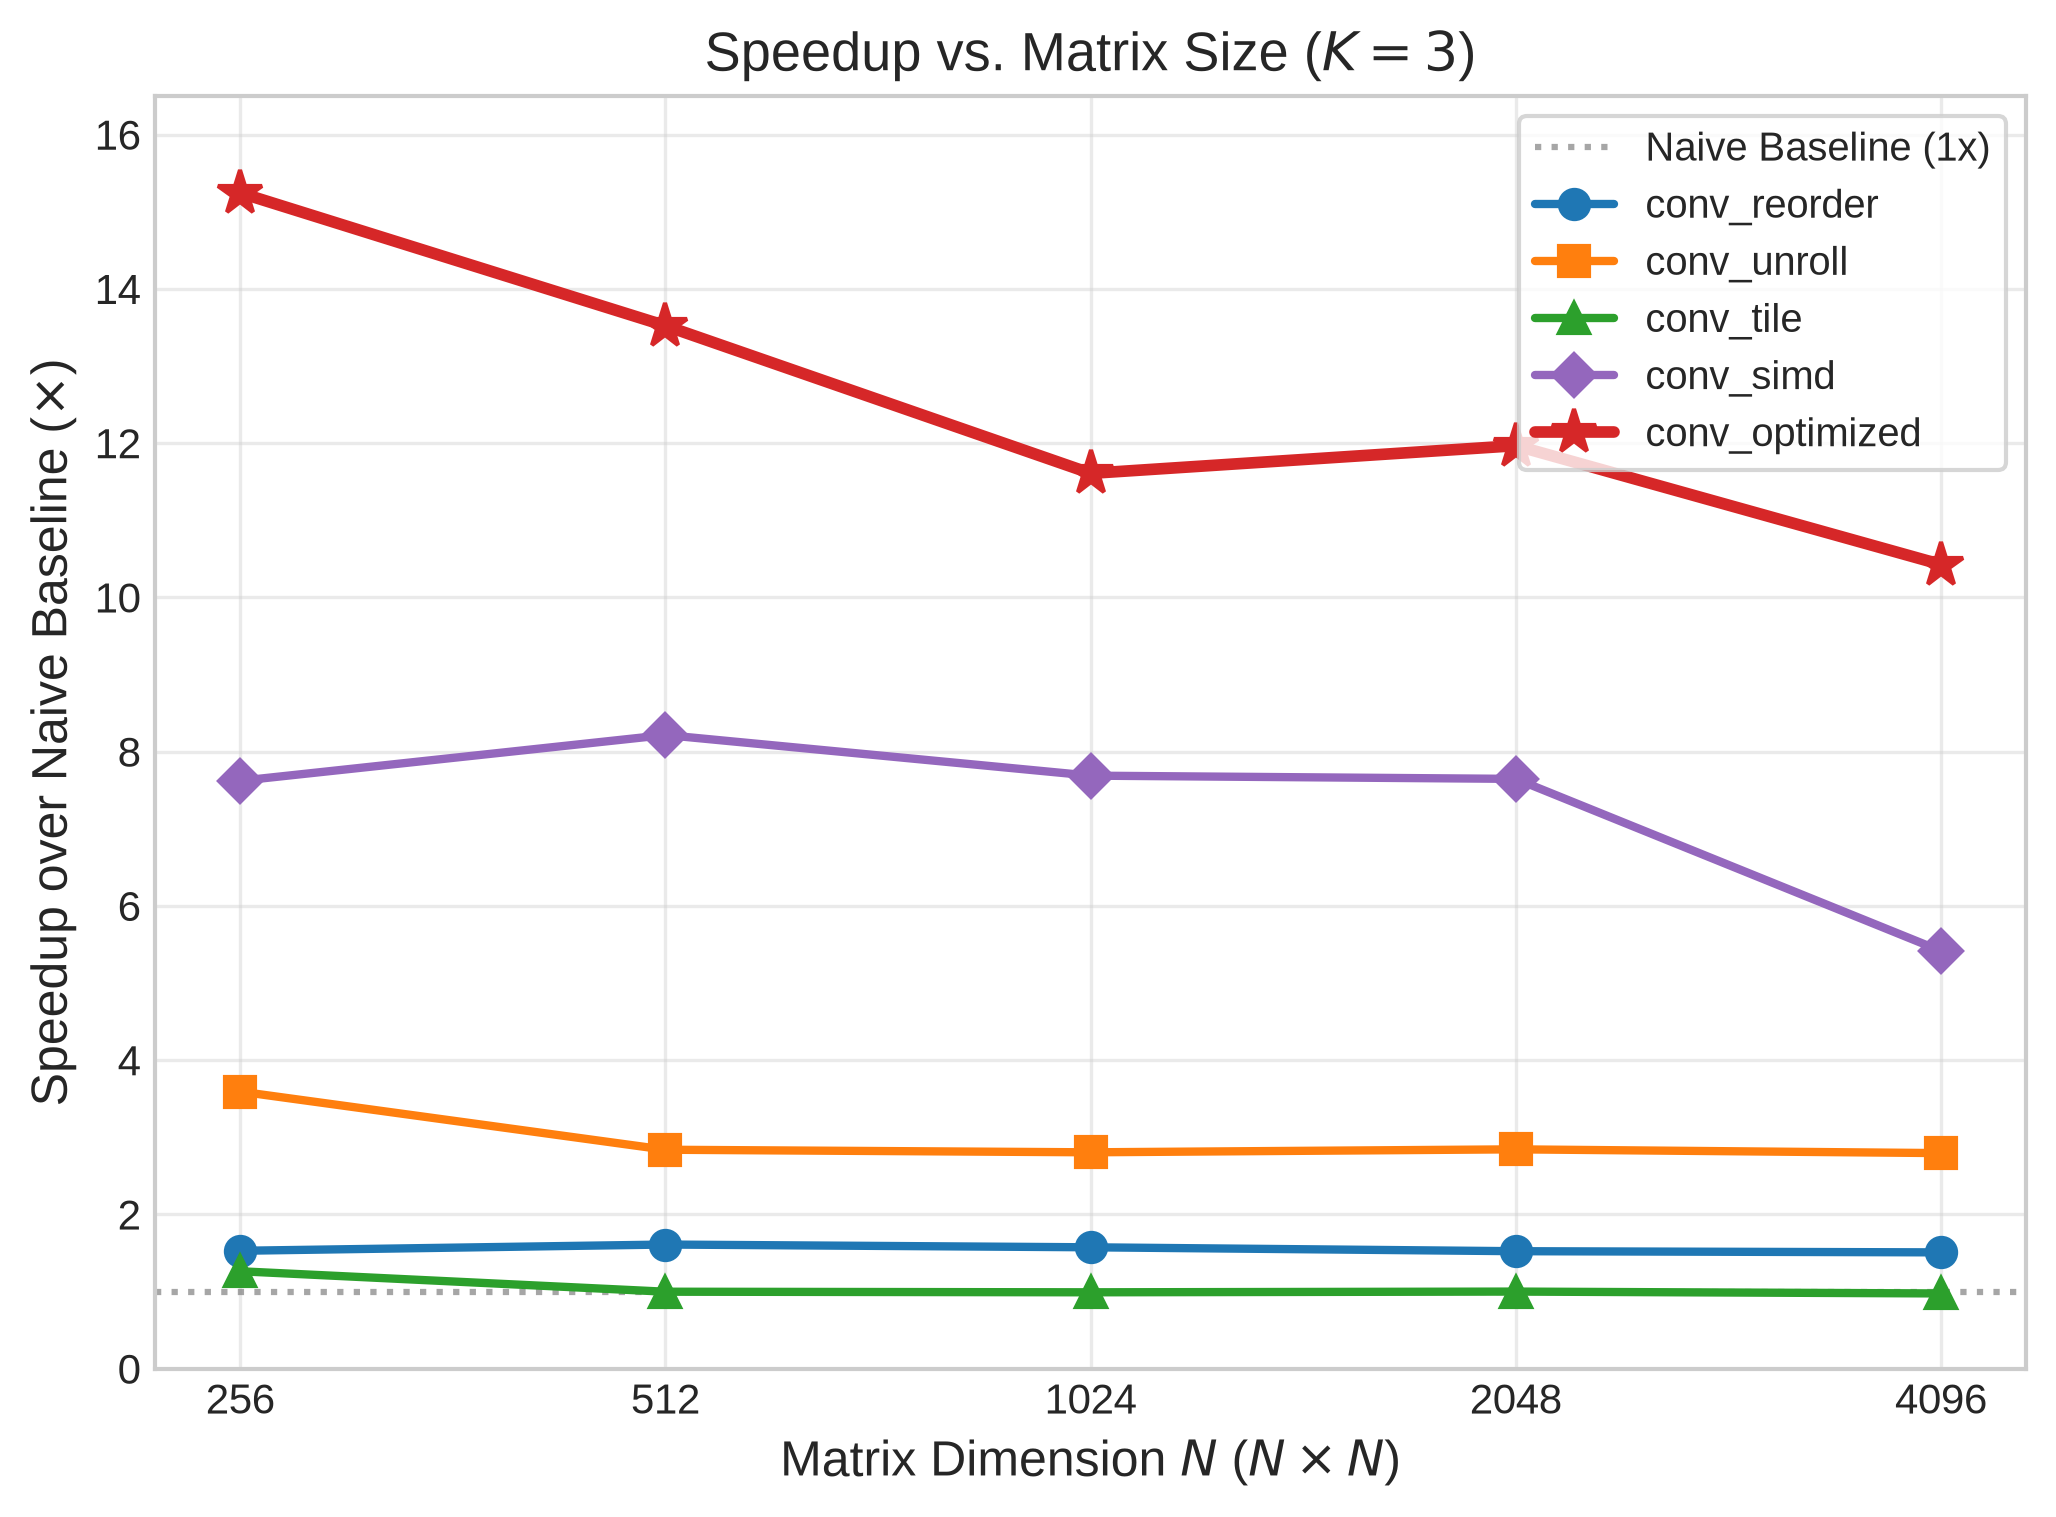
\includegraphics[width=\textwidth]{figures/1d_speedup_matrix_k3.png}\\
        {\small (a) Speedup vs. Matrix Size at $K=3$}
    \end{minipage}
    \hfill
    \begin{minipage}{0.48\textwidth}
        \centering
        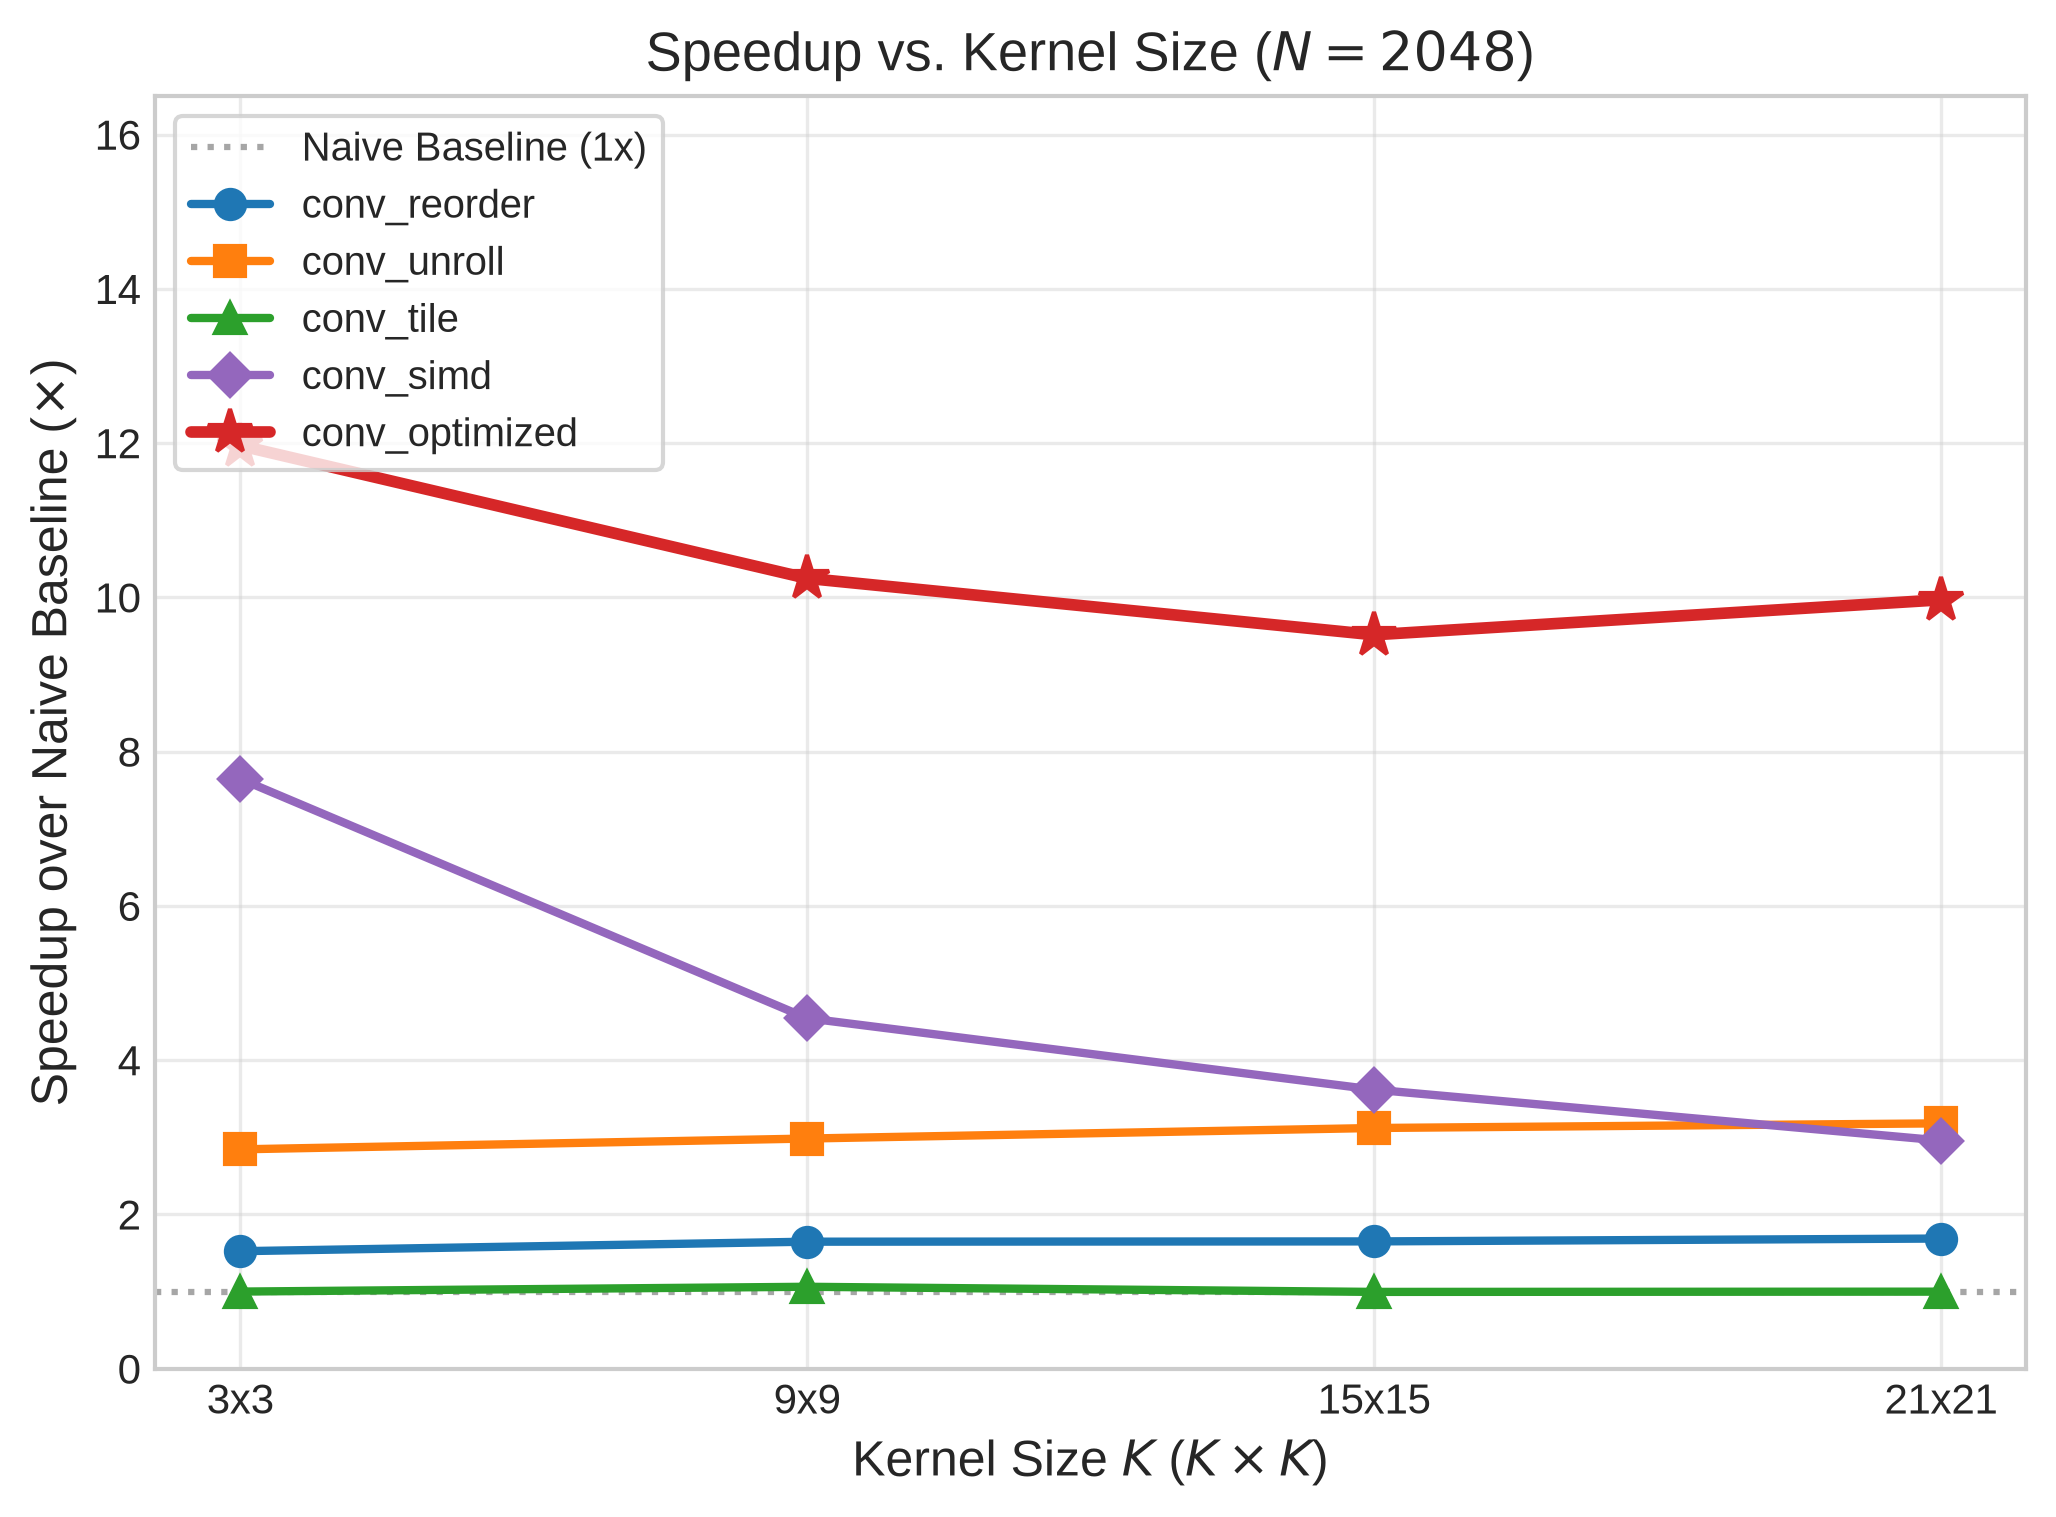
\includegraphics[width=\textwidth]{figures/1d_speedup_kernel_n2048.png}\\
        {\small (b) Speedup vs. Kernel Size at $N=2048$}
    \end{minipage}
    \caption{Task 1D: Performance scaling of all optimization stages: (a) Speedup over naive baseline across matrix dimensions ($K=3$), and (b) Speedup across kernel sizes ($N=2048$).}
    \label{fig:1d_speedup}
\end{figure}

% \clearpage
% \subsection{Justification of Observed Performance Gains Across Techniques}
% \begin{enumerate}
%     \item \textbf{Synergistic Speedup ($8.96\times$--$15.24\times$)}:
%     \begin{itemize}
%         \item \texttt{conv\_optimized} consistently achieves the highest performance across all workloads, reaching up to \textbf{$15.24\times$ speedup} over naive baseline and up to \textbf{$37.4\text{ GFLOP/s}$} sustained throughput.
%         \item The combined benefit substantially surpasses the sum of individual scalar optimizations, verifying true super-additive synergy: vectorization provides data parallelism, while multi-accumulator unrolling unlocks the execution port bandwidth needed to sustain that parallelism.
%     \end{itemize}

%     \item \textbf{Dramatic Instruction Count Collapse (Up to 94.5\% Reduction)}:
%     \begin{itemize}
%         \item At $K=21, N=4096$,  instructions drop from $48{,}937.54\times 10^6$ (naive) down to \textbf{$2{,}711.08\times 10^6$} (\texttt{conv\_optimized}), a \textbf{$94.5\%$ reduction}. At $K=9, N=4096$, instructions drop from $10{,}836.68\times 10^6$ to $1{,}451.71\times 10^6$ ($86.6\%$ reduction).
%         \item Packing 8 pixels per AVX2 vector eliminates 7 of every 8 arithmetic operations, unrolling by 64 floats eliminates 63 of every 64 loop control branches, and hardware FMA fuses multiplication and addition into a single  instruction.
%     \end{itemize}

%     \item \textbf{Latency Hiding and Clock Cycle Reduction}:
%     \begin{itemize}
%         \item In naive scalar convolution, execution cycles are dominated by RAW stalls on the single accumulator. By distributing FMAs across 8 independent vector registers, the CPU pipeline is never starved, collapsing execution clock cycles by up to \textbf{$10.2\times$}.
%     \end{itemize}

%     \item \textbf{Cache-Aware Streaming Without Boundary Penalties}:
%     \begin{itemize}
%         \item Vertical Y-tiling ensures that active input rows remain resident in the 1.25\,MB L2 cache for large images ($N=4096$) while avoiding horizontal slicing ($TX=W$), preserving contiguous streaming and maintaining low L1-D MPKI ($< 4.8$) without halo reloads.
%     \end{itemize}
% \end{enumerate}

\end{document}
